\documentclass{article}
\usepackage[
  a4paper,
  left=2cm, right=2cm,
  top=2cm, bottom=2cm
]{geometry}
\usepackage{graphicx} % Required for inserting images
\usepackage{amsmath}       % Équations avancées
\usepackage{amssymb}       % Symboles mathématiques
\usepackage{graphicx}      % Inclusion de figures
\usepackage{siunitx}       % Unités SI
\usepackage{setspace}
\singlespacing
\usepackage{multirow}
\usepackage{booktabs}      % Tableaux professionnels
\usepackage[table]{xcolor}
\usepackage{hyperref}      % Références cliquables
\usepackage[most]{tcolorbox}
\usepackage{bm}
\usepackage{float}

\usepackage[framemethod=TikZ]{mdframed}
\usepackage{pgfplots}   
\usepackage{caption}   

\usepackage{enumitem}
\usepackage{titlesec}
\usepackage{wasysym}
\usepackage{tikz}
\usetikzlibrary{positioning,arrows.meta,shapes.geometric,decorations.pathreplacing,calc,3d,positioning,patterns} % pour "below=of ..." et "-Stealth"
\usepackage{tikz-3dplot}

\usepackage{algorithm}
\usepackage{algorithmic}

\usepackage{listings}
\usetikzlibrary{shapes,arrows,positioning,calc}

\usepackage{fancyvrb}
\usepackage{fvextra}
\usepackage{pifont}

\newcommand{\codeTight}{\fontsize{8pt}{9pt}\selectfont} 

\captionsetup{font=footnotesize,labelfont=bf,textfont=it,skip=0pt}

% Commandes personnalisées
\newcommand{\cmark}{\textcolor{successgreen}{\ding{51}}}
\newcommand{\xmark}{\textcolor{errorred}{\ding{55}}}
\newcommand{\wmark}{\textcolor{warningorange}{\ding{45}}}


% --- Espaces autour des flottants (tables, figures) ---
\setlength{\textfloatsep}{8pt plus 2pt minus 2pt}
\setlength{\floatsep}{8pt plus 2pt minus 2pt}
\setlength{\intextsep}{8pt plus 2pt minus 2pt}
\setlength{\abovecaptionskip}{4pt}
\setlength{\belowcaptionskip}{0pt}

% --- Listes pour tout le document ---
\setlist[itemize]{itemsep=0pt, topsep=2pt, parsep=0pt, partopsep=0pt}
\setlist[enumerate]{itemsep=0pt, topsep=2pt, parsep=0pt, partopsep=0pt}

% --- Espaces autour des titres ---
\titlespacing*{\section}
  {0pt}{2ex plus 1ex minus .2ex}{1ex plus .5ex minus .2ex}
\titlespacing*{\subsection}
  {0pt}{1.5ex plus .5ex minus .2ex}{0.7ex plus .3ex minus .1ex}

% --- Espaces autour des formules affichées ---
\setlength{\abovedisplayskip}{6pt}
\setlength{\belowdisplayskip}{6pt}
\setlength{\abovedisplayshortskip}{4pt}
\setlength{\belowdisplayshortskip}{4pt}

\definecolor{misty}{rgb}{1.0,0.89,0.88}
\definecolor{MyBlue}{rgb}{0.8,1.0,1.0}
\definecolor{Carnelian}{rgb}{0.7,0.11,0.11}
\definecolor{MyGreen}{rgb}{0.0,0.5,0.0}
\definecolor{MyGreen2}{rgb}{0.0,0.42,0.24}
\definecolor{corrigecolor}{RGB}{180,100,200}
\definecolor{methode1color}{RGB}{220,80,60}
\definecolor{methode2color}{RGB}{80,180,80}
\definecolor{lightblue}{RGB}{220,235,255}
\definecolor{successgreen}{RGB}{39,174,96}
\definecolor{warningorange}{RGB}{243,156,18}
\definecolor{errorred}{RGB}{231,76,60}
\definecolor{infoblue}{RGB}{52,152,219}
\definecolor{darkblue}{RGB}{44,62,80}
\definecolor{lightgray}{RGB}{245,245,245}
\definecolor{purple}{RGB}{142,68,173}
\definecolor{lightgray}{RGB}{245,245,245}
\definecolor{okgreen}{RGB}{39,174,96}
\definecolor{warnorange}{RGB}{230,126,34}

% Couleurs personnalisées
\definecolor{aircolor}{RGB}{200, 220, 255}
\definecolor{tungcolor}{RGB}{255, 220, 200}
\definecolor{ratiocolor}{RGB}{220, 255, 220}

% Couleurs personnalisées
\definecolor{aircolor}{RGB}{220, 220, 220}
\definecolor{tungcolor}{RGB}{255, 220, 200}
\definecolor{pmmacolor}{RGB}{200, 255, 200}
\definecolor{ratiocolor}{RGB}{200, 220, 255}


% Définition des couleurs
\definecolor{tungsten}{RGB}{100,100,120}
\definecolor{wpetg}{RGB}{80,80,100}
\definecolor{water}{RGB}{100,180,255}
\definecolor{waterlight}{RGB}{150,200,255}
\definecolor{source}{RGB}{255,200,0}
\definecolor{cone1}{RGB}{255,100,100}
\definecolor{cone2}{RGB}{100,100,255}

\definecolor{source}{RGB}{255,200,0}
\definecolor{cone20}{RGB}{100,150,255}
\definecolor{cone60}{RGB}{255,150,100}
\definecolor{water}{RGB}{100,180,255}


% Configuration des couleurs
\definecolor{typeA}{RGB}{231,76,60}
\definecolor{typeB}{RGB}{241,196,15}
\definecolor{typeC}{RGB}{230,126,34}
\definecolor{typeD0}{RGB}{155,89,182}
\definecolor{typeD1}{RGB}{52,152,219}
\definecolor{typeD2}{RGB}{26,188,156}
\definecolor{typeD3}{RGB}{46,204,113}
\definecolor{typeD4}{RGB}{149,165,166}

\definecolor{methode1}{RGB}{70,130,180}
\definecolor{methode1bis}{RGB}{60,179,113}
\definecolor{methode2}{RGB}{255,140,0}
\definecolor{theoriecolor}{RGB}{0,100,180}

% Couleurs
\definecolor{darkblue}{RGB}{0,51,102}
\definecolor{lightblue}{RGB}{230,240,250}
\definecolor{lightgreen}{RGB}{230,250,230}
\definecolor{lightorange}{RGB}{255,240,220}
\definecolor{lightred}{RGB}{255,230,230}
\definecolor{method1}{RGB}{70,130,180}
\definecolor{method1bis}{RGB}{60,179,113}
\definecolor{method2}{RGB}{255,140,0}

% Couleurs pour la figure
\definecolor{filtercolor}{RGB}{128,128,153}
\definecolor{containercolor}{RGB}{102,102,115}
\definecolor{watercolor}{RGB}{51,153,255}
\definecolor{prefiltercolor}{RGB}{0,255,0}
\definecolor{postfiltercolor}{RGB}{255,255,0}
\definecolor{precontainercolor}{RGB}{255,128,0}
\definecolor{postcontainercolor}{RGB}{128,0,128}
\definecolor{prewatercolor}{RGB}{0,255,255}
\definecolor{postwatercolor}{RGB}{255,0,255}


% Couleurs
\definecolor{sourcecolor}{RGB}{255, 50, 50}
\definecolor{conecolor}{RGB}{255, 150, 150}
\definecolor{pmmacolor}{RGB}{255, 180, 100}
\definecolor{watercolor}{RGB}{100, 150, 255}
\definecolor{usefulcolor}{RGB}{100, 200, 100}
\definecolor{lostcolor}{RGB}{200, 200, 200}
\definecolor{solidanglecolor}{RGB}{100, 200, 100}

% Couleurs personnalisées
\definecolor{sourcecolor}{RGB}{255,100,0}
\definecolor{matrixcolor}{RGB}{255,220,100}
\definecolor{upstreamcolor}{RGB}{100,100,255}
\definecolor{downstreamcolor}{RGB}{255,100,100}
\definecolor{watercolor}{RGB}{100,180,255}
\definecolor{conecolor}{RGB}{255,200,100}
\definecolor{aircolor}{RGB}{240,248,255}
\definecolor{warningcolor}{RGB}{255,150,0}
\definecolor{energie40}{RGB}{255,100,100}
\definecolor{energie122}{RGB}{255,150,50}
\definecolor{energie344}{RGB}{255,200,50}
\definecolor{energie779}{RGB}{150,200,50}
\definecolor{energie964}{RGB}{50,200,100}
\definecolor{energie1408}{RGB}{50,150,200}

% Couleurs personnalisées
\definecolor{airblue}{RGB}{135,206,250}
\definecolor{sourcemagenta}{RGB}{255,0,255}
\definecolor{conecolor}{RGB}{255,200,0}
\definecolor{kermacolor}{RGB}{0,255,255}
\definecolor{upstreamblue}{RGB}{0,0,255}
\definecolor{downstreamred}{RGB}{255,0,0}
\definecolor{slabcolor}{RGB}{255,255,0}
\definecolor{plaquecolor}{RGB}{100,200,100}
\definecolor{cone60color}{RGB}{100,200,100}
\definecolor{cone7color}{RGB}{255,150,150}

% Couleurs personnalisées
\definecolor{precontainer}{RGB}{255,165,0}
\definecolor{postcontainer}{RGB}{0,139,139}
\definecolor{backscatter}{RGB}{148,0,211}

% Définition des couleurs
\definecolor{pmma}{RGB}{255, 180, 120}
\definecolor{water}{RGB}{100, 180, 255}
\definecolor{tungsten}{RGB}{80, 80, 80}
\definecolor{container}{RGB}{180, 180, 180}
\definecolor{preplane}{RGB}{255, 150, 50}
\definecolor{postplane}{RGB}{160, 100, 220}
\definecolor{wpetg}{RGB}{140, 140, 160}

% Définition des couleurs
\definecolor{headercolor}{RGB}{70, 130, 180}
\definecolor{successcolor}{RGB}{34, 139, 34}
\definecolor{photocolor}{RGB}{255, 200, 200}
\definecolor{comptoncolor}{RGB}{200, 200, 255}
\definecolor{paircolor}{RGB}{200, 255, 200}

% Couleurs personnalisées
\definecolor{sourcecolor}{RGB}{255,100,100}
\definecolor{slabcolor}{RGB}{255,230,100}
\definecolor{upstreamcolor}{RGB}{100,150,255}
\definecolor{downstreamcolor}{RGB}{255,100,100}
\definecolor{kermacolor}{RGB}{100,255,255}
\definecolor{aircolor}{RGB}{220,240,255}
\definecolor{conecolor}{RGB}{255,200,150}
\definecolor{worldcolor}{RGB}{240,240,240}
\definecolor{envelopecolor}{RGB}{200,220,255}

\definecolor{transmitcolor}{RGB}{46,204,113}
\definecolor{absorbcolor}{RGB}{231,76,60}
\definecolor{scattercolor}{RGB}{241,196,15}
\definecolor{oldcolor}{RGB}{180,180,180}

% Couleurs personnalisées
\definecolor{aircolor}{RGB}{200,230,255}
\definecolor{watercolor}{RGB}{100,150,255}
\definecolor{sourcecolor}{RGB}{255,80,80}
\definecolor{detectorcolor}{RGB}{100,200,100}
\definecolor{conecolor}{RGB}{255,180,100}
\definecolor{cone7color}{RGB}{100,200,255}
\definecolor{envelopecolor}{RGB}{230,230,230}
\definecolor{upstreamcolor}{RGB}{80,80,255}
\definecolor{downstreamcolor}{RGB}{255,80,80}
\definecolor{gammacolor}{RGB}{255,200,0}

% Couleurs
\definecolor{spherecolor}{RGB}{100,150,255}
\definecolor{raycolor}{RGB}{255,100,100}
\definecolor{chordcolor}{RGB}{50,200,50}
\definecolor{centercolor}{RGB}{0,0,0}
\definecolor{pointcolor}{RGB}{200,50,50}

\definecolor{wpetg}{RGB}{34,139,34}      % Vert forêt pour W/PETG
\definecolor{inox}{RGB}{192,192,192}     % Gris argent pour Inox
\definecolor{water}{RGB}{100,149,237}    % Bleu pour eau
\definecolor{source}{RGB}{255,215,0}     % Or pour source
\definecolor{gamma}{RGB}{255,69,0}       % Orange-rouge pour gammas

% Couleurs
\definecolor{lightgreen}{RGB}{220,255,220}
\definecolor{lightyellow}{RGB}{255,255,220}
\definecolor{lightblue}{RGB}{220,235,255}
\definecolor{bismuth}{RGB}{180,140,200}
\definecolor{petg}{RGB}{200,200,220}
\definecolor{eau}{RGB}{150,200,255}
\definecolor{air}{RGB}{240,248,255}
\definecolor{cone60}{RGB}{255,200,150}

\definecolor{headerblue}{RGB}{41,128,185}
\definecolor{lightgray}{RGB}{245,245,245}

\definecolor{sourcecolor}{RGB}{255, 50, 50}
\definecolor{filtercolor}{RGB}{120, 120, 140}
\definecolor{containercolor}{RGB}{100, 100, 115}
\definecolor{pmmacolor}{RGB}{255, 180, 100}
\definecolor{watercolor}{RGB}{100, 150, 255}
\definecolor{tungstencolor}{RGB}{60, 60, 60}
\definecolor{precontainercolor}{RGB}{255, 140, 0}
\definecolor{postcontainercolor}{RGB}{150, 0, 150}
\definecolor{contactcolor}{RGB}{0, 200, 0}

% Boîtes colorées
\newtcolorbox{databox}[1]{
    colback=blue!5,
    colframe=blue!75!black,
    fonttitle=\bfseries,
    title=#1
}

\newtcolorbox{resultbox}[1]{
    colback=green!5,
    colframe=green!75!black,
    fonttitle=\bfseries,
    title=#1
}

\newtcolorbox{warningbox}[1]{
    colback=orange!5,
    colframe=orange!75!black,
    fonttitle=\bfseries,
    title=#1
}

% --- Espaces autour des flottants (tables, figures) ---
\setlength{\textfloatsep}{8pt plus 2pt minus 2pt}
\setlength{\floatsep}{8pt plus 2pt minus 2pt}
\setlength{\intextsep}{8pt plus 2pt minus 2pt}
\setlength{\abovecaptionskip}{4pt}
\setlength{\belowcaptionskip}{0pt}

% --- Listes pour tout le document ---
\setlist[itemize]{itemsep=0pt, topsep=2pt, parsep=0pt, partopsep=0pt}
\setlist[enumerate]{itemsep=0pt, topsep=2pt, parsep=0pt, partopsep=0pt}

% --- Espaces autour des titres ---
\titlespacing*{\section}
  {0pt}{2ex plus 1ex minus .2ex}{1ex plus .5ex minus .2ex}
\titlespacing*{\subsection}
  {0pt}{1.5ex plus .5ex minus .2ex}{0.7ex plus .3ex minus .1ex}

% --- Espaces autour des formules affichées ---
\setlength{\abovedisplayskip}{6pt}
\setlength{\belowdisplayskip}{6pt}
\setlength{\abovedisplayshortskip}{4pt}
\setlength{\belowdisplayshortskip}{4pt}

\title{
\vspace{-1cm}
{\color{blue}\rule{\linewidth}{2pt}}\\[0.5cm]
{\Huge\bfseries Simulation Monte Carlo Geant4}\\[0.3cm]
{\Large Effet d'une Plaque W/PETG sur le Débit de Dose}\\[0.3cm]
{\large Source Eur152 - Cône 60° -25 Millions d'Événements}\\[0.3cm]
{\color{Carnelian}\rule{\linewidth}{2pt}}
}
\title{\textbf{Analyse des Méthodes de Calcul du dose\\dans une Simulation Geant4}\\[0.5cm]
\large Source Europium-152 -- Puits couronne à 20 cm -- plaque intermédiaire W/PETG (5mm) }
\author{Documentation technique}
\date{\today}

\begin{document}

\maketitle

\begin{abstract}
Ce document présente une analyse comparative de méthodes de calcul grandeurs radiométriques (débit de Kerma, débit de dose dans des tissus mous),  implémentées dans la simulation Geant4 d'une source d'Europium-152.\newline La première méthode repose sur le dépôt d'énergie Monte Carlo, tandis que la seconde utilise le calcul par fluence avec les coefficients d'absorption d'énergie tabulés. Cette analyse inclut les fondements théoriques, l'implémentation informatique et les conditions de validité de chaque approche.
\end{abstract}

\newpage

\tableofcontents

\newpage

%==============================================================================
\normalsize
\noindent \begin{mdframed}[backgroundcolor=orange!20]
\section{\Large \color{blue} \textbf{Configuration de la simulation}\color{black}}
\end{mdframed}
\footnotesize
%==============================================================================

\begin{tcolorbox}[colback=blue!5,colframe=blue,title=\textbf{Nouvelle Configuration}]
\noindent ${\rm \; \; \; \; \; \; \; \;}$ \; \textbf{-} \; Une source d'\color{blue}\textbf{Eur152}\color{black} \; de 44 KBq a une position $\bm{z}$ de 2 cm\newline
\noindent ${\rm \; \; \; \; \; \; \; \;}$ \; \textbf{-} \; Une \color{blue}\textbf{plaque intermediaire}\color{black} \; de \textbf{W/PETG} pour filtrer le rayonnement avec une épaisseur initiale de 5 mm\newline
\noindent ${\rm \; \; \; \; \; \; \; \;}$ \; \textbf{-} \; Son centre est en $\bm{z}$ = 1.75 cm, ses dimensions en $\bm{xy}$ sont de 100 $\times$ 100 mm\newline
\noindent ${\rm \; \; \; \; \; \; \; \;}$ \; \textbf{-} \; A une distance $\bm{z}$ de 78.5 mm de la source, se trouve une container de 50 mm de diamètre. L'epaisseur de ce container est de 7mm en $z$\newline
\noindent ${\rm \; \; \; \; \; \; \; \;}$ \; \textbf{-} \; Dans le container se trouve 5 couronnes d'eau concentriques de 5 mm de largeur\color{black}. La hauteur de l'eau est de 5mm
\end{tcolorbox}

%==============================================================================
\normalsize
\noindent \begin{mdframed}[backgroundcolor=orange!20]
\section{\Large \color{blue} \textbf{Description de la géométrie}\color{black}}
\end{mdframed}
\footnotesize
%==============================================================================

\begin{figure}[h!]
\centering
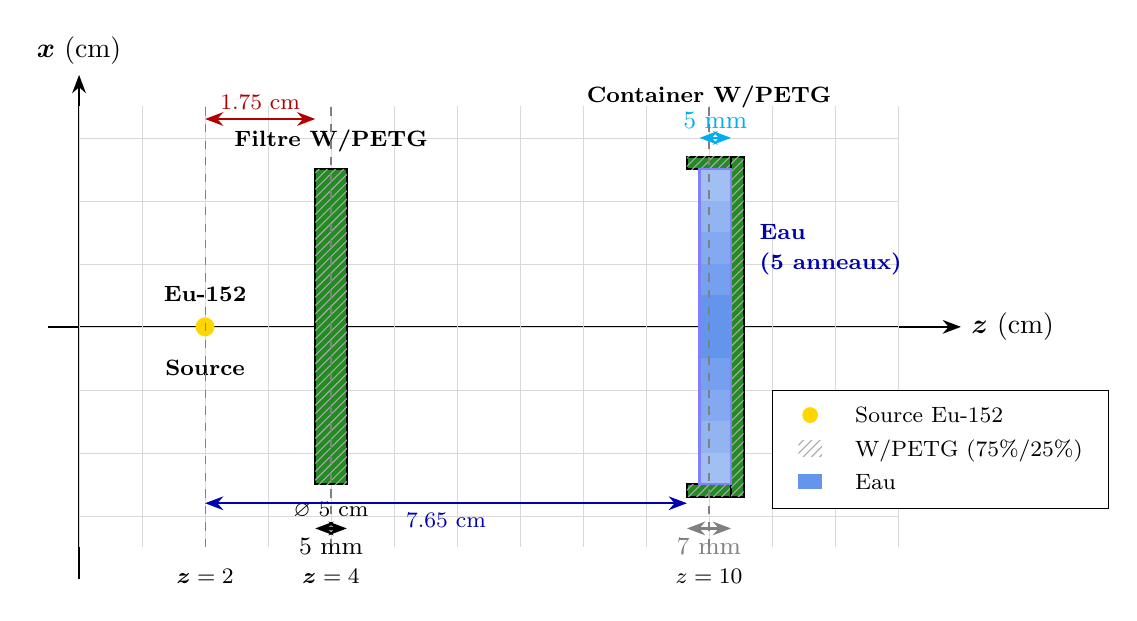
\begin{tikzpicture}[scale=0.8, >=Stealth]

    % Échelle : 1 cm dessin = 1 cm réel
    \def\sourceZ{2}
    \def\filterZ{4}
    \def\filterR{2.5}
    \def\filterThick{0.5}
    % Container : centre cavité à z=10cm, hauteur intérieure 7mm, paroi 2mm
    \def\containerCenterZ{10}
    \def\containerR{2.5}
    \def\containerWall{0.2}
    \def\containerInnerHeight{0.7}
    \def\waterThick{0.5}
    
    % Positions calculées
    % Face intérieure basse (ouverture) : 10 - 0.35 = 9.65 cm
    % Face intérieure haute (fond interne) : 10 + 0.35 = 10.35 cm
    % Face extérieure haute (fond externe) : 10.35 + 0.2 = 10.55 cm
    % Eau : de 10.35 - 0.5 = 9.85 cm à 10.35 cm (contre le fond)
    
    % Axe z
    \draw[->, thick] (-0.5,0) -- (14,0) node[right] {$\bm{z}$ (cm)};
    \draw[->, thick] (0,-4) -- (0,4) node[above] {$\bm{x}$ (cm)};
    
    % Grille de fond (optionnelle)
    \draw[very thin, gray!30] (0,-3.5) grid[step=1] (13,3.5);
    
    % =========================================================================
    % SOURCE Eu-152 à z = 2 cm
    % =========================================================================
    \fill[source] (\sourceZ, 0) circle (0.15);
    \node[below=0.3cm] at (\sourceZ, 0) {\footnotesize \textbf{Source}};
    \node[above=0.2cm] at (\sourceZ, 0) {\footnotesize \textbf{Eu-152}};
    
    % Ligne de position source
    \draw[dashed, gray] (\sourceZ, -3.5) -- (\sourceZ, 3.5);
    \node[below] at (\sourceZ, -3.7) {\footnotesize $\bm{z}=2$};
    
    % =========================================================================
    % FILTRE W/PETG à z = 4 cm (épaisseur 5 mm)
    % =========================================================================
    \fill[wpetg] (\filterZ - \filterThick/2, -\filterR) 
                 rectangle (\filterZ + \filterThick/2, \filterR);
    \draw[thick] (\filterZ - \filterThick/2, -\filterR) 
                 rectangle (\filterZ + \filterThick/2, \filterR);
    
    % Hachures pour le filtre
    \fill[pattern=north east lines, pattern color=tungsten!50] 
         (\filterZ - \filterThick/2, -\filterR) 
         rectangle (\filterZ + \filterThick/2, \filterR);
    
    \node[above=0.1cm] at (\filterZ, \filterR) {\footnotesize \textbf{Filtre W/PETG}};
    \node[below=0.1cm] at (\filterZ, -\filterR) {\footnotesize $\varnothing$ 5 cm};
    
    % Ligne de position filtre
    \draw[dashed, gray] (\filterZ, -3.5) -- (\filterZ, 3.5);
    \node[below] at (\filterZ, -3.7) {\footnotesize $\bm{z}=4$};
    
    % Cotation épaisseur filtre
    \draw[<->, thick] (\filterZ - \filterThick/2, -3.2) -- (\filterZ + \filterThick/2, -3.2);
    \node[below] at (\filterZ, -3.2) {\small 5 mm};
    
    % =========================================================================
    % CONTAINER W/PETG - centre cavité à z = 10 cm
    % Ouvert vers la source (face z- absente)
    % =========================================================================
    
    % Positions exactes
    \pgfmathsetmacro{\contInnerLowZ}{10 - 0.35}   % 9.65 cm - ouverture
    \pgfmathsetmacro{\contInnerHighZ}{10 + 0.35}  % 10.35 cm - fond interne
    \pgfmathsetmacro{\contOuterHighZ}{10.35 + 0.2} % 10.55 cm - fond externe
    \pgfmathsetmacro{\contOuterR}{2.5 + 0.2}      % 2.7 cm
    
    % Paroi latérale supérieure (x > 0)
    \fill[wpetg] (\contInnerLowZ, \containerR) 
                 rectangle (\contInnerHighZ, \contOuterR);
    \draw[thick] (\contInnerLowZ, \containerR) 
                 rectangle (\contInnerHighZ, \contOuterR);
    \fill[pattern=north east lines, pattern color=tungsten!50]
         (\contInnerLowZ, \containerR) 
         rectangle (\contInnerHighZ, \contOuterR);
    
    % Paroi latérale inférieure (x < 0)
    \fill[wpetg] (\contInnerLowZ, -\containerR) 
                 rectangle (\contInnerHighZ, -\contOuterR);
    \draw[thick] (\contInnerLowZ, -\containerR) 
                 rectangle (\contInnerHighZ, -\contOuterR);
    \fill[pattern=north east lines, pattern color=tungsten!50]
         (\contInnerLowZ, -\containerR) 
         rectangle (\contInnerHighZ, -\contOuterR);
    
    % Fond du container (à droite, z+)
    \fill[wpetg] (\contInnerHighZ, -\contOuterR) 
                 rectangle (\contOuterHighZ, \contOuterR);
    \draw[thick] (\contInnerHighZ, -\contOuterR) 
                 rectangle (\contOuterHighZ, \contOuterR);
    \fill[pattern=north east lines, pattern color=tungsten!50]
         (\contInnerHighZ, -\contOuterR) 
         rectangle (\contOuterHighZ, \contOuterR);
    
    % Label container
    \node[above=0.5cm] at (10, \contOuterR) {\footnotesize \textbf{Container W/PETG}};
    
    % =========================================================================
    % COURONNES D'EAU - CONTRE LA FACE INTÉRIEURE HAUTE
    % De z = 9.85 cm à z = 10.35 cm (5 mm d'épaisseur)
    % =========================================================================
    \pgfmathsetmacro{\waterHighZ}{10.35}          % Face haute = fond interne
    \pgfmathsetmacro{\waterLowZ}{10.35 - 0.5}     % Face basse = 9.85 cm
    
    % Anneau 4 (extérieur) : r = 20-25 mm
    \fill[water!60] (\waterLowZ, 2.0) rectangle (\waterHighZ, 2.5);
    \fill[water!60] (\waterLowZ, -2.0) rectangle (\waterHighZ, -2.5);
    
    % Anneau 3 : r = 15-20 mm
    \fill[water!70] (\waterLowZ, 1.5) rectangle (\waterHighZ, 2.0);
    \fill[water!70] (\waterLowZ, -1.5) rectangle (\waterHighZ, -2.0);
    
    % Anneau 2 : r = 10-15 mm
    \fill[water!80] (\waterLowZ, 1.0) rectangle (\waterHighZ, 1.5);
    \fill[water!80] (\waterLowZ, -1.0) rectangle (\waterHighZ, -1.5);
    
    % Anneau 1 : r = 5-10 mm
    \fill[water!90] (\waterLowZ, 0.5) rectangle (\waterHighZ, 1.0);
    \fill[water!90] (\waterLowZ, -0.5) rectangle (\waterHighZ, -1.0);
    
    % Anneau 0 (centre) : r = 0-5 mm
    \fill[water] (\waterLowZ, -0.5) rectangle (\waterHighZ, 0.5);
    
    % Contour eau
    \draw[thick, blue!50] (\waterLowZ, -2.5) rectangle (\waterHighZ, 2.5);
    
    % Label eau
    \node[right, blue!70!black] at (\contOuterHighZ + 0.1, 1.5) {\footnotesize \textbf{Eau}};
    \node[right, blue!70!black] at (\contOuterHighZ + 0.1, 1.0) {\footnotesize \textbf{(5 anneaux)}};
    
    % Ligne de position container
    \draw[dashed, gray] (10, -3.5) -- (10, 3.5);
    \node[below] at (10, -3.7) {\footnotesize $z=10$};
    
    % =========================================================================
    % COTATIONS DÉTAILLÉES
    % =========================================================================
    
    % Distance source-filtre (face d'entrée)
    \draw[<->, thick, red!70!black] (\sourceZ, 3.3) -- (\filterZ - \filterThick/2, 3.3);
    \node[above, red!70!black] at ({(\sourceZ + \filterZ - \filterThick/2)/2}, 3.3) {\footnotesize 1.75 cm};
    
    % Distance source-ouverture container
    \draw[<->, thick, blue!70!black] (\sourceZ, -2.8) -- (\contInnerLowZ, -2.8);
    \node[below, blue!70!black] at ({(\sourceZ + \contInnerLowZ)/2}, -2.8) {\footnotesize 7.65 cm};
    
    % Épaisseur eau
    \draw[<->, thick, cyan] (\waterLowZ, 3.0) -- (\waterHighZ, 3.0);
    \node[above, cyan] at ({(\waterLowZ + \waterHighZ)/2}, 3.0) {\small 5 mm};
    
    % Hauteur intérieure container
    \draw[<->, thick, gray] (\contInnerLowZ, -3.2) -- (\contInnerHighZ, -3.2);
    \node[below, gray] at (10, -3.2) {\small 7 mm};
    
    % =========================================================================
    % LÉGENDE
    % =========================================================================
    \node[draw, fill=white, anchor=north west] at (11, -1.) {
        \begin{tabular}{cl}
            \tikz\fill[source] (0,0) circle (0.1); & \footnotesize Source Eu-152 \\
            \tikz\fill[wpetg, pattern=north east lines, pattern color=tungsten!50] (0,0) rectangle (0.3,0.2); &\footnotesize W/PETG (75\%/25\%) \\
            \tikz\fill[water] (0,0) rectangle (0.3,0.2); &\footnotesize Eau \\
        \end{tabular}
    };

\end{tikzpicture}
\captionsetup{labelformat=empty}
\caption{\footnotesize Coupe longitudinale (plan $\bm{xz}$) du détecteur ``Puits Couronne''. L'eau (5 mm) est positionnée contre la face intérieure haute du container (le fond).}
\end{figure}


\begin{figure}[h!]
\centering
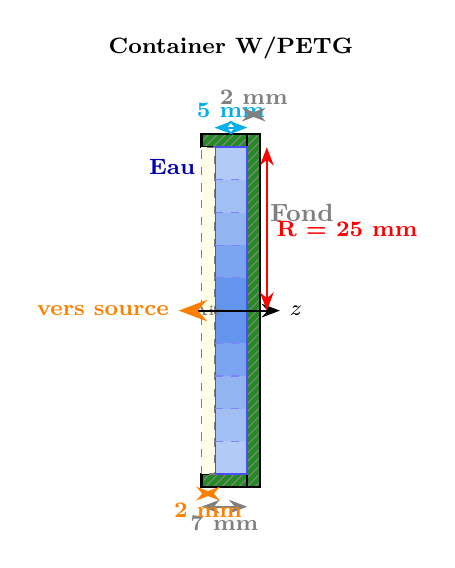
\begin{tikzpicture}[scale=8.3, >=Stealth]
    
    % Échelle agrandie : focus sur le container
    % 1 unité = 1 cm
    
    % Paramètres (en cm)
    \def\containerR{0.25}        % 2.5 cm -> 0.25 à cette échelle
    \def\containerWall{0.02}     % 2 mm
    \def\containerInnerH{0.07}   % 7 mm
    \def\waterThick{0.05}        % 5 mm
    
    % Positions Z (relatives, z=0 = ouverture)
    \def\openingZ{0}
    \def\innerTopZ{0.07}         % fond interne
    \def\outerTopZ{0.09}         % fond externe
    \def\waterBottomZ{0.02}      % 7mm - 5mm = 2mm depuis l'ouverture
    
    % =========================================================================
    % CONTAINER W/PETG
    % =========================================================================
    
    % Paroi latérale haute (x > 0)
    \fill[wpetg] (\openingZ, \containerR) rectangle (\innerTopZ, {\containerR + \containerWall});
    \fill[pattern=north east lines, pattern color=tungsten!70]
         (\openingZ, \containerR) rectangle (\innerTopZ, {\containerR + \containerWall});
    \draw[thick] (\openingZ, \containerR) rectangle (\innerTopZ, {\containerR + \containerWall});
    
    % Paroi latérale basse (x < 0)
    \fill[wpetg] (\openingZ, -\containerR) rectangle (\innerTopZ, {-\containerR - \containerWall});
    \fill[pattern=north east lines, pattern color=tungsten!70]
         (\openingZ, -\containerR) rectangle (\innerTopZ, {-\containerR - \containerWall});
    \draw[thick] (\openingZ, -\containerR) rectangle (\innerTopZ, {-\containerR - \containerWall});
    
    % Fond (à droite)
    \fill[wpetg] (\innerTopZ, {-\containerR - \containerWall}) rectangle (\outerTopZ, {\containerR + \containerWall});
    \fill[pattern=north east lines, pattern color=tungsten!70]
         (\innerTopZ, {-\containerR - \containerWall}) rectangle (\outerTopZ, {\containerR + \containerWall});
    \draw[thick] (\innerTopZ, {-\containerR - \containerWall}) rectangle (\outerTopZ, {\containerR + \containerWall});
    
    % =========================================================================
    % EAU - CONTRE LE FOND INTERNE
    % =========================================================================
    
    % L'eau va de z = innerTopZ - waterThick à z = innerTopZ
    \pgfmathsetmacro{\waterLowZ}{\innerTopZ - \waterThick}
    
    % Anneau 4 : r = 20-25 mm (0.20 - 0.25)
    \fill[water!50] (\waterLowZ, 0.20) rectangle (\innerTopZ, 0.25);
    \fill[water!50] (\waterLowZ, -0.20) rectangle (\innerTopZ, -0.25);
    
    % Anneau 3 : r = 15-20 mm
    \fill[water!60] (\waterLowZ, 0.15) rectangle (\innerTopZ, 0.20);
    \fill[water!60] (\waterLowZ, -0.15) rectangle (\innerTopZ, -0.20);
    
    % Anneau 2 : r = 10-15 mm
    \fill[water!70] (\waterLowZ, 0.10) rectangle (\innerTopZ, 0.15);
    \fill[water!70] (\waterLowZ, -0.10) rectangle (\innerTopZ, -0.15);
    
    % Anneau 1 : r = 5-10 mm
    \fill[water!85] (\waterLowZ, 0.05) rectangle (\innerTopZ, 0.10);
    \fill[water!85] (\waterLowZ, -0.05) rectangle (\innerTopZ, -0.10);
    
    % Anneau 0 : r = 0-5 mm
    \fill[water] (\waterLowZ, -0.05) rectangle (\innerTopZ, 0.05);
    
    % Contour eau
    \draw[thick, blue!70] (\waterLowZ, -0.25) rectangle (\innerTopZ, 0.25);
    
    % Lignes de séparation des anneaux
    \foreach \r in {0.05, 0.10, 0.15, 0.20} {
        \draw[thin, blue!50, dashed] (\waterLowZ, \r) -- (\innerTopZ, \r);
        \draw[thin, blue!50, dashed] (\waterLowZ, -\r) -- (\innerTopZ, -\r);
    }
    
    % =========================================================================
    % ESPACE VIDE (air) entre ouverture et eau
    % =========================================================================
    \fill[yellow!10] (\openingZ, -0.25) rectangle (\waterLowZ, 0.25);
    \draw[thin, gray, dashed] (\openingZ, -0.25) rectangle (\waterLowZ, 0.25);
    \node[gray, font=\tiny] at ({(\openingZ + \waterLowZ)/2}, 0) {\textbf{Air}};
    
    % =========================================================================
    % AXES ET COTATIONS
    % =========================================================================
    
    % Axe z
    \draw[->, thick] (-0.02, 0) -- (0.12, 0) node[right] {\footnotesize $z$};
    
    % Cotation épaisseur eau (5 mm)
    \draw[<->, thick, cyan] (\waterLowZ, 0.28) -- (\innerTopZ, 0.28);
    \node[above, cyan, font=\footnotesize] at ({(\waterLowZ + \innerTopZ)/2}, 0.28) {\textbf{5 mm}};
    
    % Cotation hauteur intérieure (7 mm)
    \draw[<->, thick, gray] (\openingZ, -0.30) -- (\innerTopZ, -0.30);
    \node[below, gray, font=\footnotesize] at ({(\openingZ + \innerTopZ)/2}, -0.30) {\textbf{7 mm}};
    
    % Cotation épaisseur fond (2 mm)
    \draw[<->, thick, gray] (\innerTopZ, 0.30) -- (\outerTopZ, 0.30);
    \node[above, gray, font=\footnotesize] at ({(\innerTopZ + \outerTopZ)/2}, 0.30) {\textbf{2 mm}};
    
    % Cotation rayon intérieur
    \draw[<->, thick, red] (0.10, 0) -- (0.10, 0.25);
    \node[right, red, font=\footnotesize] at (0.10, 0.125) {\textbf{R = 25 mm}};
    
    % Cotation espace air (2 mm)
    \draw[<->, thick, orange] (\openingZ, -0.28) -- (\waterLowZ, -0.28);
    \node[below, orange, font=\footnotesize] at ({(\openingZ + \waterLowZ)/2}, -0.28) {\textbf{2 mm}};
    
    % =========================================================================
    % LABELS
    % =========================================================================
    
    \node[above, font=\footnotesize] at (0.045, 0.37) {\textbf{Container W/PETG} };
    \node[blue!70!black, font=\footnotesize] at (-0.045, 0.22) {\textbf{Eau}};
    
    % Flèche indiquant la direction de la source
    \draw[->, ultra thick, orange] (-0.015, 0) -- (-0.035, 0);
    \node[left, orange, font=\footnotesize] at (-0.035, 0) {\textbf{vers source}};
    
    % Annotation fond
    \node[right, font=\small, gray] at (\outerTopZ, 0.15) {\textbf{Fond}};

\end{tikzpicture}
\captionsetup{labelformat=empty}
\caption{\footnotesize Vue détaillée du container ``Puits Couronne''. La tranche d'eau de 5 mm est positionnée contre la face intérieure haute (fond) du container. Un espace de 2 mm d'air sépare l'eau de l'ouverture.}
\end{figure}

\noindent \begin{mdframed}[backgroundcolor=orange!20]
\subsection{\color{blue}\textbf{Vue de face des couronnes d'eau (plan xy)}\color{black}}
\end{mdframed}
\footnotesize

\begin{figure}[h!]
\centering
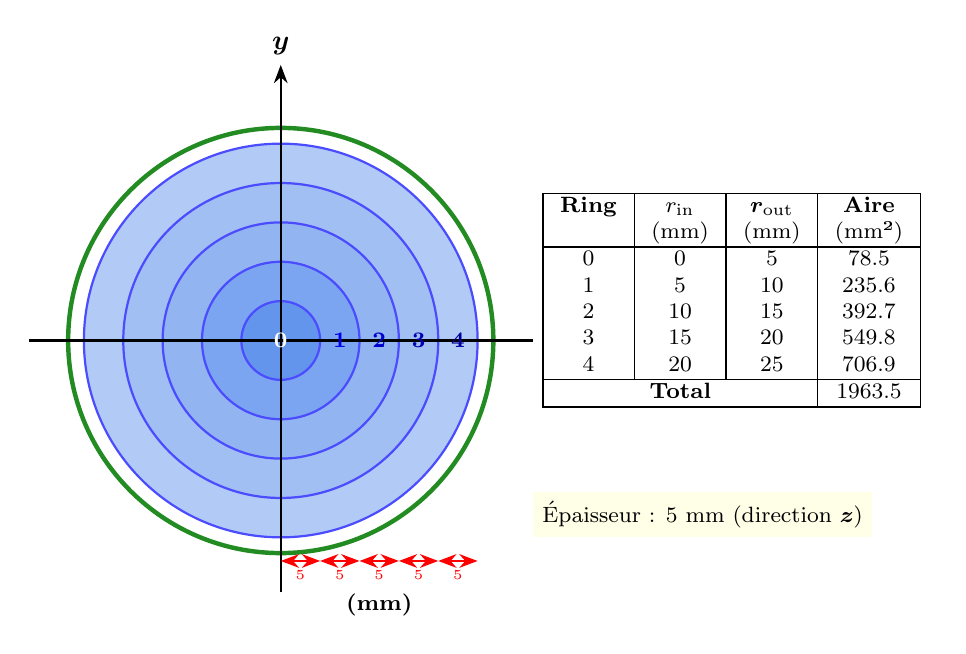
\begin{tikzpicture}[scale=1, >=Stealth]

    % Vue de face (plan xy) des couronnes d'eau
    
    % Anneau 4 (extérieur) : r = 20-25 mm
    \fill[water!50] (0,0) circle (2.5);
    
    % Anneau 3 : r = 15-20 mm
    \fill[water!60] (0,0) circle (2.0);
    
    % Anneau 2 : r = 10-15 mm
    \fill[water!70] (0,0) circle (1.5);
    
    % Anneau 1 : r = 5-10 mm
    \fill[water!85] (0,0) circle (1.0);
    
    % Anneau 0 (centre) : r = 0-5 mm
    \fill[water] (0,0) circle (0.5);
    
    % Cercles de séparation
    \draw[thick, blue!70] (0,0) circle (0.5);
    \draw[thick, blue!70] (0,0) circle (1.0);
    \draw[thick, blue!70] (0,0) circle (1.5);
    \draw[thick, blue!70] (0,0) circle (2.0);
    \draw[thick, blue!70] (0,0) circle (2.5);
    
    % Container (paroi externe)
    \draw[ultra thick, wpetg] (0,0) circle (2.7);
    
    % Axes
    \draw[->, thick] (-3.2,0) -- (3.5,0) node[right] {$\bm{x}$};
    \draw[->, thick] (0,-3.2) -- (0,3.5) node[above] {$\bm{y}$};
    
    % Labels des anneaux
    \node[white, font=\footnotesize\bfseries] at (0,0) {0};
    \node[blue!90!black, font=\footnotesize\bfseries] at (0.75,0) {\textbf{1}};
    \node[blue!80!black, font=\footnotesize\bfseries] at (1.25,0) {\textbf{2}};
    \node[blue!70!black, font=\footnotesize\bfseries] at (1.75,0) {\textbf{3}};
    \node[blue!60!black, font=\footnotesize\bfseries] at (2.25,0) {\textbf{4}};
    
    % Cotations des rayons
    \draw[<->, thick, red] (0, -2.8) -- (0.5, -2.8);
    \node[below, red, font=\tiny] at (0.25, -2.8) {5};
    
    \draw[<->, thick, red] (0.5, -2.8) -- (1.0, -2.8);
    \node[below, red, font=\tiny] at (0.75, -2.8) {5};
    
    \draw[<->, thick, red] (1.0, -2.8) -- (1.5, -2.8);
    \node[below, red, font=\tiny] at (1.25, -2.8) {5};
    
    \draw[<->, thick, red] (1.5, -2.8) -- (2.0, -2.8);
    \node[below, red, font=\tiny] at (1.75, -2.8) {5};
    
    \draw[<->, thick, red] (2.0, -2.8) -- (2.5, -2.8);
    \node[below, red, font=\tiny] at (2.25, -2.8) {5};
    
    \node[below, font=\footnotesize] at (1.25, -3.1) {\textbf{(mm)}};
    
    % Tableau des caractéristiques
    \node[fill=white, anchor=north west, align=left] at (3.2, 2.) {
        \footnotesize
        \begin{tabular}{|c|c|c|c|}
        \hline
        \footnotesize \textbf{Ring} &\footnotesize $r_{\text{in}}$&\footnotesize $\bm{r_{\text{out}}}$&\footnotesize \textbf{Aire}\\
        &\footnotesize (mm)&\footnotesize (mm)&\footnotesize  (mm²) \\
        \hline
        \footnotesize 0&\footnotesize 0&\footnotesize 5&\footnotesize 78.5 \\
        \footnotesize 1&\footnotesize 5&\footnotesize 10&\footnotesize 235.6 \\
        \footnotesize 2&\footnotesize 10&\footnotesize 15&\footnotesize 392.7 \\
        \footnotesize 3&\footnotesize 15&\footnotesize 20&\footnotesize 549.8 \\
        \footnotesize 4&\footnotesize 20&\footnotesize 25&\footnotesize 706.9 \\
        \hline
        \multicolumn{3}{|c|}{\footnotesize \textbf{Total}} &\footnotesize  1963.5 \\
        \hline
        \end{tabular}
    };
    
    % Note épaisseur
    \node[fill=yellow!10, anchor=south west] at (3.2, -2.5) {
        \footnotesize
        Épaisseur : 5 mm (direction $\bm{z}$)
    };

\end{tikzpicture}
\captionsetup{labelformat=empty}
\caption{\footnotesize Vue de face (plan $\bm{xy}$) des 5 couronnes d'eau concentriques. Chaque anneau a une largeur radiale de 5 mm.}
\end{figure}

\noindent \begin{mdframed}[backgroundcolor=orange!20]
\subsection{\color{blue}\textbf{Récapitulatif des positions (axe z)}\color{black}}
\end{mdframed}
\footnotesize

\noindent \footnotesize \textbf{Distance source $\rightarrow$ face d'entrée de l'eau :} $9.85 - 2.0 = 7.85$ cm

\begin{center}
\begin{tabular}{|l|c|l|}
\hline
\footnotesize \textbf{Élément}&\footnotesize \textbf{Position z}&\footnotesize \textbf{Notes} \\
\hline
\footnotesize Source Eu-152&\footnotesize 2.0 cm&\footnotesize Point source \\
\hline
\footnotesize Filtre W/PETG (face entrée)&\footnotesize 3.75 cm& \\
\footnotesize Filtre W/PETG (centre)&\footnotesize 4.0 cm&\footnotesize Épaisseur 5 mm \\
\footnotesize Filtre W/PETG (face sortie)&\footnotesize 4.25 cm& \\
\hline
\footnotesize Container (ouverture)&\footnotesize 9.65 cm&\footnotesize Face ouverte vers source \\
\footnotesize Container (centre cavité)&\footnotesize 10.0 cm&\footnotesize Hauteur int. 7 mm \\
\footnotesize Container (fond interne)&\footnotesize 10.35 cm& \\
\footnotesize Container (fond externe)&\footnotesize 10.55 cm&\footnotesize Épaisseur fond 2 mm \\
\hline
\footnotesize Eau (face basse)&\footnotesize 9.85 cm&\footnotesize Vers la source \\
\footnotesize Eau (face haute)&\footnotesize 10.35 cm&\footnotesize Contre le fond interne \\
\hline
\end{tabular}
\end{center}

\noindent \begin{mdframed}[backgroundcolor=orange!20]
\subsection{\color{blue}\textbf{Visualisation des angles solides}\color{black}}
\end{mdframed}
\footnotesize

\begin{figure}[h!]
\centering
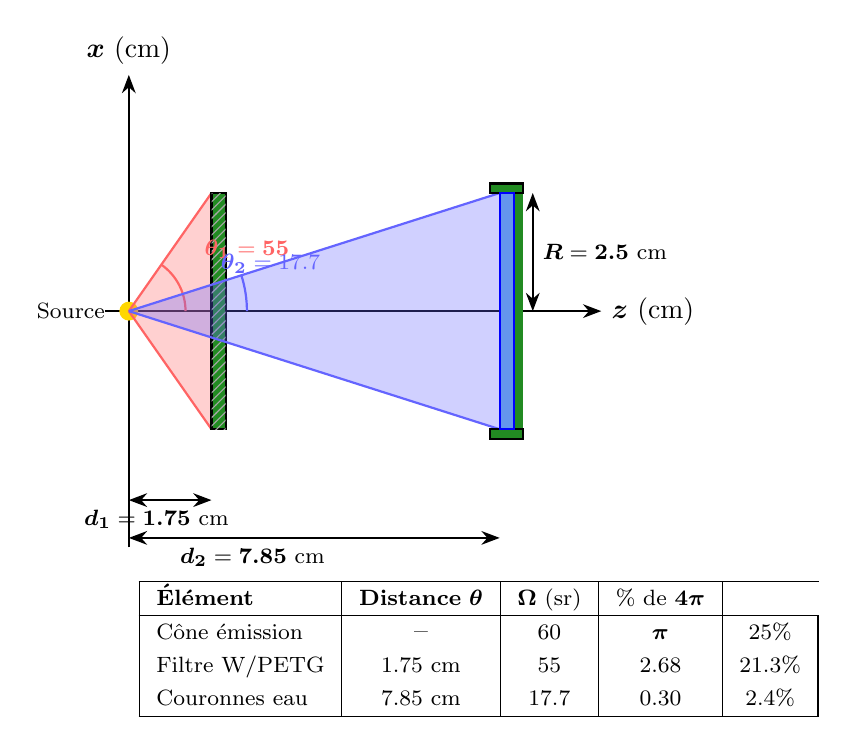
\begin{tikzpicture}[scale=0.6, >=Stealth, baseline=(current bounding box.center)]

    % Échelle adaptée pour visualiser les cônes
    \def\sourceZ{0}
    \def\filterZ{1.75}
    \def\filterR{2.5}
    \def\containerZ{7.65}
    \def\containerR{2.5}
    % Distance source -> face d'entrée de l'eau = 7.65 + 0.2 = 7.85 cm
    \def\waterZ{7.85}
    
    % Axe z
    \draw[->, thick] (-0.5,0) -- (10,0) node[right] {$\bm{z}$ (cm)};
    \draw[->, thick] (0,-5) -- (0,5) node[above] {$\bm{x}$ (cm)};
    
    % =========================================================================
    % SOURCE
    % =========================================================================
    \fill[source] (\sourceZ, 0) circle (0.2);
    \node[left] at (-0.3, 0) {\footnotesize Source};
    
    % =========================================================================
    % CÔNE VERS LE FILTRE (θ = 55°)
    % =========================================================================
    \def\filterAngle{55}
    
    % Remplissage du cône vers filtre
    \fill[cone1, opacity=0.3] (\sourceZ, 0) 
        -- (\filterZ, \filterR)
        -- (\filterZ, -\filterR)
        -- cycle;
    
    % Bords du cône vers filtre
    \draw[thick, cone1] (\sourceZ, 0) -- (\filterZ, \filterR);
    \draw[thick, cone1] (\sourceZ, 0) -- (\filterZ, -\filterR);
    
    % Filtre
    \fill[wpetg] (\filterZ, -\filterR) rectangle ({\filterZ + 0.3}, \filterR);
    \draw[thick] (\filterZ, -\filterR) rectangle ({\filterZ + 0.3}, \filterR);
    \fill[pattern=north east lines, pattern color=tungsten!50] 
         (\filterZ, -\filterR) rectangle ({\filterZ + 0.3}, \filterR);
    
    % Arc pour l'angle vers filtre
    \draw[thick, cone1] (1.2, 0) arc (0:\filterAngle:1.2);
    \node[cone1, above right] at (1.4, 0.9) {\footnotesize $\bm{\theta_1} = \bm{55}°$};
    
    % =========================================================================
    % CÔNE VERS L'EAU (θ = 17.7°)
    % Distance source-eau = 7.85 cm
    % =========================================================================
    \def\waterAngle{17.7}
    
    % Remplissage du cône vers eau
    \fill[cone2, opacity=0.3] (\sourceZ, 0) 
        -- (\waterZ, \containerR)
        -- (\waterZ, -\containerR)
        -- cycle;
    
    % Bords du cône vers eau
    \draw[thick, cone2] (\sourceZ, 0) -- (\waterZ, \containerR);
    \draw[thick, cone2] (\sourceZ, 0) -- (\waterZ, -\containerR);
    
    % Container (simplifié)
    \fill[wpetg] (\containerZ, \containerR) rectangle ({\containerZ + 0.7}, {\containerR + 0.2});
    \fill[wpetg] (\containerZ, -\containerR) rectangle ({\containerZ + 0.7}, {-\containerR - 0.2});
    \fill[wpetg] ({\containerZ + 0.5}, {-\containerR - 0.2}) rectangle ({\containerZ + 0.7}, {\containerR + 0.2});
    \draw[thick] (\containerZ, \containerR) rectangle ({\containerZ + 0.7}, {\containerR + 0.2});
    \draw[thick] (\containerZ, -\containerR) rectangle ({\containerZ + 0.7}, {-\containerR - 0.2});
    
    % Eau (contre le fond)
    \fill[water] ({\containerZ + 0.2}, -\containerR) rectangle ({\containerZ + 0.5}, \containerR);
    \draw[thick, blue] ({\containerZ + 0.2}, -\containerR) rectangle ({\containerZ + 0.5}, \containerR);
    
    % Arc pour l'angle vers eau
    \draw[thick, cone2] (2.5, 0) arc (0:\waterAngle:2.5);
    \node[cone2, above] at (3.0, 0.6) {\footnotesize $\bm{\theta_2} = 17.7°$};
    
    % =========================================================================
    % ANNOTATIONS DISTANCES
    % =========================================================================
    
    % Distance source-filtre
    \draw[<->, thick] (\sourceZ, -4) -- (\filterZ, -4);
    \node[below] at ({(\sourceZ + \filterZ)/3}, -4) {\footnotesize $\bm{d_1} = \bm{1.75}$ cm};
    
    % Distance source-eau
    \draw[<->, thick] (\sourceZ, -4.8) -- (\waterZ, -4.8);
    \node[below] at ({(\sourceZ + \waterZ)/3}, -4.8) {\footnotesize $\bm{d_2} = \bm{7.85}$ cm};
    
    % Rayon
    \draw[<->, thick] ({\containerZ + 0.9}, 0) -- ({\containerZ + 0.9}, \containerR);
    \node[right] at ({\containerZ + 0.9}, \containerR/2) {\footnotesize $\bm{R} = \bm{2.5}$ cm};
    
    % =========================================================================
    % TABLEAU  
    % =========================================================================
    \node[fill=white, anchor=north west, align=left] at (0, -5.5) {
    \begin{tabular}{|l|c|c|c|c|}
    \hline
    \footnotesize \textbf{Élément}&\footnotesize \textbf{Distance} \footnotesize $\bm{\theta}$&\footnotesize $\bm{\Omega}$ (sr) &\footnotesize \% de $\bm{4\pi}$ \\
     \hline
     \footnotesize Cône émission & -- &\footnotesize $60°$ &\footnotesize $\bm{\pi}$ &\footnotesize 25\% \\
     \footnotesize Filtre W/PETG &\footnotesize 1.75 cm &\footnotesize $55°$ &\footnotesize 2.68 &\footnotesize 21.3\% \\
     \footnotesize Couronnes eau &\footnotesize 7.85 cm &\footnotesize $17.7°$ &\footnotesize 0.30 &\footnotesize 2.4\% \\
     \hline
        \end{tabular}
    };
\end{tikzpicture}
\captionsetup{labelformat=empty}
\caption{\footnotesize Visualisation des cônes d'angle solide depuis la source. La distance source-eau (7.85 cm) tient compte du positionnement de l'eau contre le fond interne du container.}
\end{figure}

%==============================================================================
\normalsize
\noindent \begin{mdframed}[backgroundcolor=orange!20]
\section{\Large \color{blue} \textbf{Angles solides et normalisation}\color{black}}
\end{mdframed}
\footnotesize
%==============================================================================

\noindent La source Eu-152 a une activité de $\bm{}A = 44$ kBq sur $4\pi$ stéradians (émission isotrope). Cependant, pour optimiser le temps de calcul de la simulation Monte Carlo, on souhaite restreindre l'émission des gammas dans un cône de demi-angle $\theta_{\text{cone}} = 20°$ dirigé vers le détecteur (couronnes d'eau).\par

\begin{tcolorbox}[colback=blue!5,colframe=blue,title=\textbf{Question}]
\noindent Comment relier les résultats obtenus avec $\bm{N_{\text{sim}}}$ événements simulés dans le cône de 20° à un temps d'irradiation réel correspondant à la source isotrope de 44 kBq ?
\end{tcolorbox}

\normalsize
\noindent \begin{mdframed}[backgroundcolor=orange!20]
\subsection{\color{blue}\textbf{Définition des angles solides}\color{black}}
\end{mdframed}
\footnotesize
\medskip

\noindent L'angle solide $\bm{\Omega}$ d'un cône de demi-angle $\bm{\theta}$ vu depuis son sommet est :

\begin{equation*}
\bm{\Omega} = \bm{2\pi} \left(\bm{1} - \cos\bm{\theta}\right)
\end{equation*}

\normalsize
\noindent \color{blue}\textbf{Cône de 20° (simulation optimisée)}\color{black}
\footnotesize

\begin{align*}
\bm{\Omega_{20°}} &= \bm{2\pi} \left(\bm{1} - \cos \bm{20}°\right) \\
&= \bm{2\pi} \left(\bm{1} - \bm{0.9397}\right) \\
&= \bm{2\pi} \times \bm{0.0603} \\
&= \bm{0.379} \text{ sr}
\end{align*}

\normalsize
\noindent \color{blue}\textbf{Sphère complète}\color{black}
\footnotesize

\begin{equation*}
\bm{\Omega_{4\pi}} = \bm{4\pi} = \bm{12.566} \text{ sr}
\end{equation*}

\noindent La fraction de l'émission $\bm{4\pi}$ couverte par le cône de 20 degré est :

\begin{equation*}
\bm{f} = \frac{\bm{\Omega_{20}}}{\bm{\Omega_{4\pi}}} = \frac{\bm{0.379}}{\bm{12.566}} = \bm{0.0302} = \bm{3.02}\%
\end{equation*}

\begin{center}
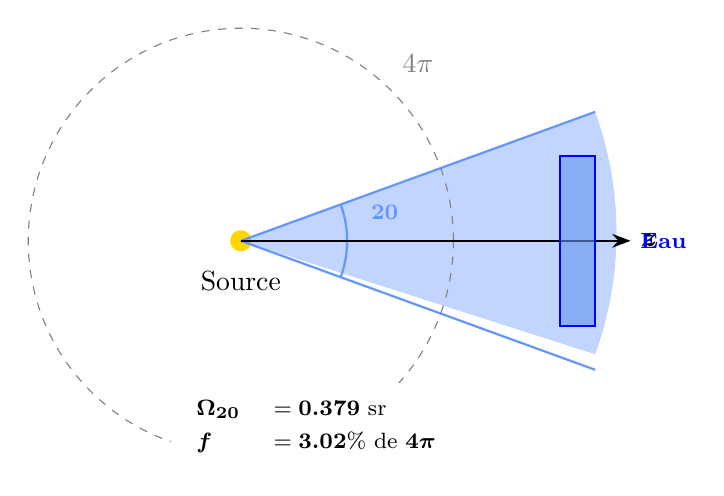
\begin{tikzpicture}[scale=0.9, >=Stealth]
    % Source
    \fill[source] (0,0) circle (0.15);
    \node[below] at (0, -0.3) {Source};
    
    % Cône 20°
    \fill[cone20, opacity=0.4] (0,0) -- (5, {5*tan(20)}) arc (20:-20:5) -- cycle;
    \draw[thick, cone20] (0,0) -- (5, {5*tan(20)});
    \draw[thick, cone20] (0,0) -- (5, {-5*tan(20)});
    
    % Arc 20°
    \draw[thick, cone20] (1.5, 0) arc (0:20:1.5);
    \draw[thick, cone20] (1.5, 0) arc (0:-20:1.5);
    \node[cone20, right] at (1.7, 0.4) {\footnotesize $\bm{20}$};
    
    % Sphère 4π (représentation partielle)
    \draw[dashed, gray] (0,0) circle (3);
    \node[gray] at (2.5, 2.5) {$4\pi$};
    
    % Axe
    \draw[->, thick] (0,0) -- (5.5, 0) node[right] {$\bm{z}$};
    
    % Eau (cible)
    \fill[water, opacity=0.6] (4.5, -1.2) rectangle (5, 1.2);
    \draw[thick, blue] (4.5, -1.2) rectangle (5, 1.2);
    \node[blue, right] at (5.5, 0) {\footnotesize \textbf{Eau}};
    
    % Annotations
    \node[fill=white, anchor=north west] at (-1, -2) {
        \begin{tabular}{ll}
        \footnotesize$ \bm{\Omega_{20°}}$ &\footnotesize $= \bm{0.379}$ sr \\
        \footnotesize$\bm{f}$ &\footnotesize $= \bm{3.02}\%$ de $\bm{4\pi}$
        \end{tabular}
    };
\end{tikzpicture}
\end{center}

\normalsize
\noindent \begin{mdframed}[backgroundcolor=orange!20]
\subsection{\color{blue}\textbf{Principe de la renormalisation}\color{black}}
\end{mdframed}
\footnotesize
\medskip

\normalsize
\noindent \color{blue}\textbf{Équivalence physique}\color{black}
\footnotesize

\noindent Lorsqu'on simule $\bm{N_{\text{sim}}}$ événements (désintégrations) dans un cône de demi-angle $\bm{\theta_{\text{cone}}}$, on échantillonne uniquement la fraction $\bm{f}$ de l'émission totale.

\begin{tcolorbox}[colback=blue!5,colframe=blue,title=\textbf{Principe fondamental}]
\noindent Ces $\bm{N_{\text{sim}}}$ événements dans le cône correspondent au même nombre de gammas qu'une source isotrope aurait émis dans ce même cône après avoir effectué $\bm{N_{4\pi}}$ désintégrations sur $\bm{4\pi}$
\end{tcolorbox}

\begin{equation*}
\bm{N_{4\pi}} = \frac{\bm{N_{\text{sim}}}}{\bm{f}}
\end{equation*}

\begin{itemize}
\item $\bm{N_{\text{sim}}}$ = nombre d'événements simulés dans le cône
\item $\bm{N_{4\pi}}$ = nombre équivalent de désintégrations de la source isotrope
\item $\bm{f}$ = fraction de l'angle solide ($\bm{\Omega_{\text{cone}}} / \bm{4\pi}$)
\end{itemize}

\noindent \textbf{Exemple :} Si on simule $\bm{N_{\text{sim}}} = \bm{100\,000}$ événements dans un cône de 20° :

\begin{equation*}
\bm{N_{4\pi}} = \frac{\bm{100\,000}}{\bm{0.0302}} = \bm{3.31} \times \bm{10^6} \text{ désintégrations sur } \bm{4\pi}
\end{equation*}

\normalsize
\noindent \begin{mdframed}[backgroundcolor=orange!20]
\subsection{\color{blue}\textbf{Calcul du temps d'irradiation}\color{black}}
\end{mdframed}
\footnotesize

\normalsize
\noindent \color{blue}\textbf{Relation activité -- temps}\color{black}
\footnotesize

\noindent L'activité $\bm{A}$ de la source est définie comme le nombre de désintégrations par seconde :

\begin{equation*}
\bm{A} = \frac{\bm{N_{\text{désintégrations}}}}{\bm{\Delta t}}
\end{equation*}

\noindent Donc le temps correspondant à $\bm{N_{4\pi}}$ désintégrations est :
\begin{equation*}
\bm{T_{\text{irr}}} = \frac{\bm{N_{4\pi}}}{\bm{A}} = \frac{\bm{N_{\text{sim}}}}{\bm{f} \cdot \bm{A}}
\end{equation*}

\noindent \color{blue}\textbf{Prise en compte du nombre de gammas par désintégration}\color{black}
\footnotesize

\noindent Pour l'Eu-152, chaque désintégration produit en moyenne $\bm{\bar{n}_\gamma} = \bm{1.924}$ gammas (dans le spectre considéré). Si la simulation génère des \textit{gammas} (et non des désintégrations), il faut en tenir compte :

\begin{equation*}
\bm{T_{\text{irr}}} = \frac{\bm{N_{\text{sim}}}}{\bm{f} \cdot \bm{A} \cdot \bm{\bar{n}_\gamma}}
\end{equation*}

\normalsize
\noindent \color{blue}\textbf{Application numérique}\color{black}
\footnotesize

\begin{center}
\begin{tabular}{ll}
\toprule
\footnotesize \textbf{Paramètre} &\footnotesize  \textbf{Valeur} \\
\midrule
\footnotesize Activité $\bm{A}$ &\footnotesize  $44\,000$ Bq \\
\footnotesize Demi-angle du cône $\theta$ &\footnotesize  $\bm{20}°$ \\
\footnotesize Fraction $\bm{f}$ &\footnotesize  $\bm{0.0302}$ \\
\footnotesize Gammas par désintégration $\bm{\bar{n}_\gamma}$ &\footnotesize  $\bm{1.924}$ \\
\bottomrule
\end{tabular}
\end{center}

\normalsize
\noindent \color{blue}\textbf{Temps par événement simulé}\color{black}
\footnotesize

\begin{align*}
\bm{t_1} &= \frac{\bm{1}}{\bm{f} \cdot \bm{A} \cdot \bm{\bar{n}_\gamma}} \\
&= \frac{\bm{1}}{\bm{0.0302} \times \bm{44\,000} \times \bm{1.924}} \\
&= \frac{\bm{1}}{\bm{2556}} \text{ s} \\
&= \bm{0.391} \text{ ms par événement}
\end{align*}

\normalsize
\noindent \color{blue}\textbf{Temps pour $\bm{N_{\text{sim}}}$ événements}\color{black}
\footnotesize

\begin{equation*}
\bm{T_{\text{irr}}} = \bm{N_{\text{sim}}} \times \bm{0.391} \text{ ms}
\end{equation*}

\begin{center}
\begin{tabular}{rr}
\toprule
\footnotesize $\bm{N_{\text{sim}}}$ &\footnotesize  $\bm{T_{\text{irr}}}$ \\
\midrule
\footnotesize $\bm{10\,000}$ &\footnotesize  $\bm{3.91}$ s \\
\footnotesize $\bm{100\,000}$ &\footnotesize  $\bm{39.1}$ s \\
\footnotesize $\bm{1\,000\,000}$ &\footnotesize  $\bm{6.52}$ min \\
\footnotesize $\bm{10\,000\,000}$ &\footnotesize  $\bm{1.09}$ h \\
\bottomrule
\end{tabular}
\end{center}

\normalsize
\noindent \begin{mdframed}[backgroundcolor=orange!20]
\subsection{\color{blue}\textbf{Formules récapitulatives}\color{black}}
\end{mdframed}
\footnotesize

\normalsize
\noindent \color{blue}\textbf{Formule générale du temps d'irradiation}\color{black}
\footnotesize

\begin{equation*}
\bm{T_{\text{irr}}} = \frac{\bm{N_{\text{sim}}} \cdot \bm{4\pi}}{\bm{2\pi}(\bm{1}-\cos\bm{\theta_{\text{cone}}}) \cdot \bm{A} \cdot \bm{\bar{n}_\gamma}} = \frac{\bm{2} \cdot \bm{N_{\text{sim}}}}{(\bm{1}-\cos\bm{\theta_{\text{cone}}}) \cdot \bm{A} \cdot \bm{\bar{n}_\gamma}}
\end{equation*}

\normalsize
\noindent \color{blue}\textbf{Formule du débit de dose}\color{black}
\footnotesize

\noindent Si la simulation donne une dose totale $\bm{D_{\text{sim}}}$ (en Gy) pour $\bm{N_{\text{sim}}}$ événements, le débit de dose est :

\begin{equation*}
\bm{\dot{D}} = \frac{\bm{D_{\text{sim}}}}{\bm{T_{\text{irr}}}} = \frac{\bm{D_{\text{sim}}} \cdot \bm{f} \cdot \bm{A} \cdot \bm{\bar{n}_\gamma}}{\bm{N_{\text{sim}}}}
\end{equation*}

\normalsize
\noindent \color{blue}\textbf{Vérification dimensionnelle}\color{black}
\footnotesize

\begin{align*}
[\bm{\dot{D}}] &= \frac{[\bm{\text{Gy}}] \times [\bm{\text{sr}}] \times [\bm{\text{Bq}}] \times [\bm{1}]}{[\bm{\text{sr}}] \times [\bm{1}]} \\
&= \frac{\bm{\text{Gy}} \times \bm{\text{s}}^{-1}}{1} = \text{Gy/s}
\end{align*}

\normalsize
\noindent \begin{mdframed}[backgroundcolor=orange!20]
\subsection{\color{blue}\textbf{Implémentation dans le code Geant4}\color{black}}
\end{mdframed}
\footnotesize

\normalsize
\noindent \color{blue}\textbf{Calcul automatique dans RunAction}\color{black}
\footnotesize
\smallskip

\noindent Modifier \color{blue}\textbf{RunAction.cc}\color{black} \; pour calculer le temps d'irradiation correct :

\begin{verbatim}
// Paramètres
G4double coneAngle = 20.0 * deg;           // Demi-angle du cône
G4double activity = 44000.0;               // Bq
G4double gammasPerDecay = 1.924;

// Fraction de l'angle solide
G4double f = (1.0 - std::cos(coneAngle)) / 2.0;

// Temps d'irradiation
G4double T_irr = nofEvents / (f * activity * gammasPerDecay);
\end{verbatim}

\newpage

%==============================================================================
\normalsize
\noindent \begin{mdframed}[backgroundcolor=orange!20]
\section{\Large \color{blue} \textbf{Structure des données ROOT}\color{black}}
\end{mdframed}
\footnotesize
%==============================================================================

\begin{tcolorbox}[colback=blue!5,colframe=blue,title=\textbf{Principe fondamental}]
\noindent Ces $\bm{N_{\text{sim}}}$ événements dans le cône correspondent au même nombre de gammas qu'une source isotrope aurait émis dans ce même cône après avoir effectué $\bm{N_{4\pi}}$ désintégrations sur $\bm{4\pi}$
\end{tcolorbox}

\begin{tcolorbox}[colback=blue!5,colframe=blue]
\noindent Le fichier ROOT \color{blue}\textbf{puits\_couronne\_output.root}\color{black} \; contient :
\begin{itemize}
    \item \color{blue}\textbf{9 histogrammes}\color{black} \; (H0 à H8)
    \item \color{blue}\textbf{3 ntuples}\color{black} (EventData, GammaData, RingDoseData)
\end{itemize}

\noindent Ces données sont enregistrées pour chaque run de simulation et permettent une analyse détaillée de :
\begin{itemize}
    \item La \color{blue}\textbf{génération des gammas primaires}\color{black} \; (spectre Eu-152)
    \item La \color{blue}\textbf{transmission à travers le filtre W/PETG}\color{black}
    \item La \color{blue}\textbf{dose déposée dans les 5 anneaux d'eau}\color{black}
\end{itemize}
\end{tcolorbox}


\normalsize
\noindent \begin{mdframed}[backgroundcolor=orange!20]
\subsection{\color{blue}\textbf{Histogrammes}\color{black}}
\end{mdframed}
\footnotesize
\medskip

\normalsize
\noindent \color{blue}\textbf{Liste des histogrammes}\color{black}
\footnotesize
\smallskip

\begin{table}[h!]
\centering
\renewcommand{\arraystretch}{1.3}
\begin{tabular}{|c|l|c|c|c|}
\hline
\rowcolor{headerblue}
\footnotesize \textcolor{white}{\textbf{ID}}&\footnotesize  \textcolor{white}{\textbf{Nom}}&\footnotesize  \textcolor{white}{\textbf{Bins}}&\footnotesize  \textcolor{white}{\textbf{Min}}&\footnotesize  \textcolor{white}{\textbf{Max}} \\
\hline
\footnotesize \color{headerblue}\textbf{H0}\color{black} &\footnotesize \texttt{nGammasPerEvent}&\footnotesize 15&\footnotesize $-0.5$&\footnotesize $14.5$ \\
\hline
\footnotesize \color{headerblue}\textbf{H1}\color{black}&\footnotesize \texttt{energySpectrum}&\footnotesize 1500&\footnotesize 0&\footnotesize  1500 keV \\
\hline
\footnotesize \color{headerblue}\textbf{H2}\color{black}&\footnotesize \texttt{totalEnergyPerEvent}&\footnotesize 500&\footnotesize 0&\footnotesize  5000 keV \\
\hline
\footnotesize \color{headerblue}\textbf{H3}\color{black}&\footnotesize \texttt{doseRing0}&\footnotesize 200&\footnotesize 0&\footnotesize  200 keV\\
\hline
\footnotesize \color{headerblue}\textbf{H4}\color{black}&\footnotesize \texttt{doseRing1}&\footnotesize 200&\footnotesize 0 &\footnotesize  200 keV\\
\hline
\footnotesize \color{headerblue}\textbf{H5}\color{black}&\footnotesize \texttt{doseRing2}&\footnotesize 200&\footnotesize 0&\footnotesize 200 keV\\
\hline
\footnotesize \color{headerblue}\textbf{H6}\color{black}&\footnotesize \texttt{doseRing3}&\footnotesize 200&\footnotesize 0 &\footnotesize  200 keV\\
\hline
\footnotesize \color{headerblue}\textbf{H7}\color{black}&\footnotesize \texttt{doseRing4}&\footnotesize 200&\footnotesize 0 &\footnotesize  200 keV\\
\hline
\footnotesize \color{headerblue}\textbf{H8}\color{black}&\footnotesize \texttt{doseTotalWater}&\footnotesize 500&\footnotesize 0&\footnotesize  500 keV\\
\hline
\end{tabular}
\captionsetup{labelformat=empty}
\caption{\footnotesize Liste des histogrammes dans le fichier ROOT}
\end{table}

\normalsize
\noindent \color{blue}\textbf{Description détaillée}\color{black}
\footnotesize
\medskip

\noindent \color{headerblue}\textbf{H0 : nGammasPerEvent}\color{black}
\begin{tcolorbox}[colback=lightgray,colframe=headerblue,title=Nombre de gammas par événement]
\color{headerblue}\textbf{Description :}\color{black} \; Distribution du nombre de gammas primaires générés par désintégration.\\
\color{headerblue}\textbf{Remplissage :}\color{black} \; \texttt{RunAction::RecordEventStatistics()}\\
\color{headerblue}\textbf{Valeur attendue :}\color{black} \; Moyenne $\bm{\bar{n}_\gamma} \approx \bm{1.924}$ (spectre Eu-152)
\end{tcolorbox}

\noindent \color{headerblue}\textbf{H1 : energySpectrum}\color{black}
\begin{tcolorbox}[colback=lightgray,colframe=headerblue,title=Spectre en énergie des gammas]
\color{headerblue}\textbf{Description :}\color{black} \; Spectre des énergies de tous les gammas primaires générés.\\
\color{headerblue}\textbf{Remplissage :}\color{black} \; \texttt{RunAction::RecordEventStatistics()}\\
\color{headerblue}\textbf{Raies principales :} 40, 122, 245, 344, 779, 964, 1112, 1408 keV
\end{tcolorbox}

\noindent \color{headerblue}\textbf{H2 : totalEnergyPerEvent}\color{black}
\begin{tcolorbox}[colback=lightgray,colframe=headerblue,title=Énergie totale par événement]
\color{headerblue}\textbf{Description :}\color{black} \; Somme des énergies de tous les gammas primaires par désintégration.\\
\color{headerblue}\textbf{Remplissage :}\color{black} \; \texttt{RunAction::RecordEventStatistics()}
\end{tcolorbox}

\noindent \color{headerblue}\textbf{H3--H7 : doseRing0 à doseRing4}\color{black}
\begin{tcolorbox}[colback=lightgray,colframe=headerblue,title=Dose par anneau d'eau]
\color{headerblue}\textbf{Description :}\color{black} \; Distribution des dépôts d'énergie (en keV) dans chaque anneau d'eau, par désintégration.\\
\color{headerblue}\textbf{Remplissage :}\color{black} \; \texttt{RunAction::AddRingEnergy()}\\[0.5em]
\begin{tabular}{|c|c|c|}
\hline
\footnotesize \textbf{Histo}&\footnotesize \textbf{Anneau}&\footnotesize \textbf{Rayon (mm)} \\
\hline
\footnotesize H3&\footnotesize Ring 0&\footnotesize  $r = 0-5$ \\
\footnotesize H4&\footnotesize Ring 1&\footnotesize  $r = 5-10$ \\
\footnotesize H5&\footnotesize Ring 2&\footnotesize  $r = 10-15$ \\
\footnotesize H6&\footnotesize Ring 3&\footnotesize  $r = 15-20$ \\
\footnotesize H7&\footnotesize Ring 4&\footnotesize  $r = 20-25$ \\
\hline
\end{tabular}
\end{tcolorbox}

\noindent \color{headerblue}\textbf{H8 : doseTotalWater}\color{black}
\begin{tcolorbox}[colback=lightgray,colframe=headerblue,title=Dose totale dans l'eau]
\color{headerblue}\textbf{Description :}\color{black} \; Distribution de l'énergie totale déposée dans l'ensemble des anneaux d'eau, par désintégration.\\
\color{headerblue}\textbf{Remplissage :}\color{black} \; \texttt{RunAction::RecordEventStatistics()}\\
\color{headerblue}\textbf{Condition :}\color{black} \; Uniquement si $E_{dep} > 0$
\end{tcolorbox}

\normalsize
\noindent \begin{mdframed}[backgroundcolor=orange!20]
\subsection{\color{blue}\textbf{Ntuples}\color{black}}
\end{mdframed}
\footnotesize
\medskip

\normalsize
\noindent \color{blue}\textbf{Ntuple 0 : EventData}\color{black}
\footnotesize
\smallskip
\begin{tcolorbox}[colback=lightgray,colframe=headerblue,title=Données par événement (désintégration)]
\color{headerblue}\textbf{Description :}\color{black} \; Une ligne par événement (désintégration simulée).\\
\color{headerblue}\textbf{Remplissage :}\color{black} \; \texttt{EventAction::EndOfEventAction()}
\end{tcolorbox}

\begin{table}[h!]
\centering
\renewcommand{\arraystretch}{1.2}
\begin{tabular}{|c|l|c|p{7cm}|}
\hline
\rowcolor{headerblue}
\footnotesize \textcolor{white}{\textbf{Col}}&\footnotesize \textcolor{white}{\textbf{Nom}}&\footnotesize \textcolor{white}{\textbf{Type}}&\footnotesize \textcolor{white}{\textbf{Description}} \\
\hline
\footnotesize \color{headerblue}\textbf{0}\color{black} &\footnotesize \texttt{eventID}&\footnotesize Int&\footnotesize Numéro de l'événement \\
\hline
\footnotesize \color{headerblue}\textbf{1}\color{black} &\footnotesize \texttt{nPrimaries}&\footnotesize Int&\footnotesize Nombre de gammas primaires générés \\
\hline
\footnotesize \color{headerblue}\textbf{2}\color{black} &\footnotesize \texttt{totalEnergy}&\footnotesize Double&\footnotesize Énergie totale des primaires (keV) \\
\hline
\footnotesize \color{headerblue}\textbf{3}\color{black} &\footnotesize  \texttt{nTransmitted}&\footnotesize Int&\footnotesize Nombre de gammas transmis à travers le filtre \\
\hline
\footnotesize \color{headerblue}\textbf{4}\color{black} &\footnotesize \texttt{nAbsorbed}&\footnotesize Int&\footnotesize Nombre de gammas absorbés par le filtre \\
\hline
\footnotesize \color{headerblue}\textbf{5}\color{black} &\footnotesize \texttt{nScattered}&\footnotesize Int&\footnotesize Nombre de gammas diffusés (Compton) \\
\hline
\footnotesize \color{headerblue}\textbf{6}\color{black} &\footnotesize  \texttt{nSecondaries}&\footnotesize Int&\footnotesize Nombre de particules secondaires détectées \\
\hline
\footnotesize \color{headerblue}\textbf{7}\color{black} &\footnotesize \texttt{totalWaterDeposit}&\footnotesize Double&\footnotesize Énergie déposée dans l'eau (keV) \\
\hline
\end{tabular}
\captionsetup{labelformat=empty}
\caption{\footnotesize Structure du ntuple EventData}
\end{table}

\normalsize
\noindent \color{blue}\textbf{Ntuple 1 : GammaData}\color{black}
\footnotesize
\smallskip

\begin{tcolorbox}[colback=lightgray,colframe=headerblue,title=Données par gamma primaire]
\color{headerblue}\textbf{Description :}\color{black} Une ligne par gamma primaire émis.\\
\color{headerblue}\textbf{Remplissage :}\color{black} \; \texttt{EventAction::EndOfEventAction()}
\end{tcolorbox}


\begin{tcolorbox}[colback=lightgray,colframe=headerblue,title={Critère de transmission}]
\noindent Un gamma est considéré comme transmis si :

\begin{equation*}
\left| \bm{E_{\text{upstream}}} - \bm{E_{\text{downstream}}} \right| < \bm{1} \text{ keV}
\end{equation*}
\end{tcolorbox}

\newpage 

\begin{table}[h!]
\centering
\renewcommand{\arraystretch}{1.2}
\begin{tabular}{|c|l|c|p{6.5cm}|}
\hline
\rowcolor{headerblue}
\footnotesize \textcolor{white}{\textbf{Col}}&\footnotesize \textcolor{white}{\textbf{Nom}}&\footnotesize \textcolor{white}{\textbf{Type}} &\footnotesize \textcolor{white}{\textbf{Description}} \\
\hline
\footnotesize \color{headerblue}\textbf{0}\color{black}&\footnotesize \texttt{eventID}&\footnotesize Int&\footnotesize Numéro de l'événement parent\\
\hline
\footnotesize \color{headerblue}\textbf{1}\color{black}&\footnotesize \texttt{gammaIndex}&\footnotesize Int&\footnotesize Index du gamma dans l'événement (0, 1, 2, ...)\\
\hline
\footnotesize \color{headerblue}\textbf{2}\color{black}&\footnotesize \texttt{energyInitial}&\footnotesize Double&\footnotesize Énergie initiale (keV)\\
\hline
\footnotesize \color{headerblue}\textbf{3}\color{black}&\footnotesize \texttt{energyUpstream}&\footnotesize Double&\footnotesize Énergie au plan upstream (keV)\\
\hline
\footnotesize \color{headerblue}\textbf{4}\color{black}&\footnotesize \texttt{energyDownstream}&\footnotesize Double&\footnotesize Énergie au plan downstream (keV)\\
\hline
\footnotesize \color{headerblue}\textbf{5}\color{black}&\footnotesize \texttt{theta}&\footnotesize Double&\footnotesize Angle polaire d'émission (deg)\\
\hline
\footnotesize \color{headerblue}\textbf{6}\color{black}&\footnotesize \texttt{phi}&\footnotesize Double&\footnotesize Angle azimutal d'émission (deg)\\
\hline
\footnotesize \color{headerblue}\textbf{7}\color{black} &\footnotesize  \texttt{detectedUpstream} &\footnotesize  Int &\footnotesize  Détecté au plan upstream (0/1) \\
\hline
\footnotesize \color{headerblue}\textbf{8}\color{black} &\footnotesize  \texttt{detectedDownstream} &\footnotesize  Int &\footnotesize  Détecté au plan downstream (0/1) \\
\hline
\footnotesize \color{headerblue}\textbf{9}\color{black} &\footnotesize  \texttt{transmitted} &\footnotesize  Int &\footnotesize  Transmis sans perte d'énergie (0/1) \\
\hline
\end{tabular}
\captionsetup{labelformat=empty}
\caption{\footnotesize Structure du ntuple GammaData}
\end{table}


\normalsize
\noindent \color{blue}\textbf{Ntuple 2 : RingDoseData}\color{black}
\footnotesize
\smallskip

\begin{tcolorbox}[colback=lightgray,colframe=headerblue,title=Dose par anneau par désintégration]
\color{headerblue}\textbf{Description :}\color{black} Une ligne par événement avec la dose déposée dans chaque anneau.\\
\color{headerblue}\textbf{Remplissage :}\color{black} \texttt{EventAction::EndOfEventAction()}
\end{tcolorbox}

\begin{table}[h!]
\centering
\renewcommand{\arraystretch}{1.2}
\begin{tabular}{|c|l|c|p{6cm}|}
\hline
\rowcolor{headerblue}
\footnotesize \textcolor{white}{\textbf{Col}} &\footnotesize  \textcolor{white}{\textbf{Nom}} &\footnotesize  \textcolor{white}{\textbf{Type}} &\footnotesize  \textcolor{white}{\textbf{Description}} \\
\hline
\footnotesize \color{headerblue}\textbf{0}\color{black} &\footnotesize \texttt{eventID} &\footnotesize  Int &\footnotesize  Numéro de l'événement \\
\hline
\footnotesize \color{headerblue}\textbf{1}\color{black} &\footnotesize  \texttt{nPrimaries} &\footnotesize  Int &\footnotesize  Nombre de gammas primaires \\
\hline
\footnotesize \color{headerblue}\textbf{2}\color{black} &\footnotesize  \texttt{doseRing0} &\footnotesize  Double &\footnotesize  Énergie déposée dans Ring 0 (keV) \\
\hline
\footnotesize \color{headerblue}\textbf{3}\color{black} &\footnotesize  \texttt{doseRing1} &\footnotesize  Double &\footnotesize  Énergie déposée dans Ring 1 (keV) \\
\hline
\footnotesize \color{headerblue}\textbf{4}\color{black} &\footnotesize  \texttt{doseRing2} &\footnotesize  Double &\footnotesize  Énergie déposée dans Ring 2 (keV) \\
\hline
\footnotesize \color{headerblue}\textbf{5}\color{black} &\footnotesize  \texttt{doseRing3} &\footnotesize  Double &\footnotesize  Énergie déposée dans Ring 3 (keV) \\
\hline
\footnotesize \color{headerblue}\textbf{6}\color{black} &\footnotesize  \texttt{doseRing4} &\footnotesize  Double &\footnotesize  Énergie déposée dans Ring 4 (keV) \\
\hline
\footnotesize \color{headerblue}\textbf{7}\color{black} &\footnotesize  \texttt{doseTotal} &\footnotesize  Double &\footnotesize  Énergie totale déposée dans l'eau (keV) \\
\hline
\end{tabular}
\captionsetup{labelformat=empty}
\caption{\footnotesize Structure du ntuple RingDoseData}
\end{table}

\normalsize
\noindent \begin{mdframed}[backgroundcolor=orange!20]
\subsection{\color{blue}\textbf{Flux de données}\color{black}}
\end{mdframed}
\footnotesize
\medskip

\normalsize
\noindent \color{blue}\textbf{Diagramme de remplissage}\color{black}
\footnotesize
\smallskip

\begin{center}
\begin{tabular}{|l|l|l|}
\hline
\rowcolor{headerblue}
\footnotesize \textcolor{white}{\textbf{Classe}} &\footnotesize  \textcolor{white}{\textbf{Méthode}} &\footnotesize  \textcolor{white}{\textbf{Données remplies}} \\
\hline
\multirow{2}{*}{\footnotesize \color{headerblue}\textbf{SteppingAction}\color{black}} &\footnotesize  \texttt{UserSteppingAction()} &\footnotesize  Détection dans les plans \\
& &\footnotesize  Dépôts d'énergie $\rightarrow$ EventAction \\
\hline
\multirow{5}{*}{\footnotesize \color{headerblue}\textbf{EventAction}\color{black}} &\footnotesize  \texttt{BeginOfEventAction()} &\footnotesize  Reset des compteurs \\
& &\footnotesize  Enregistrement des primaires \\
\cline{2-3}
& \texttt{EndOfEventAction()} &\footnotesize  Ntuple 0 (EventData) \\
& &\footnotesize  Ntuple 1 (GammaData) \\
& &\footnotesize  Ntuple 2 (RingDoseData) \\
\hline
\multirow{2}{*}{\footnotesize \color{headerblue}\textbf{RunAction}\color{black}} &\footnotesize  \texttt{RecordEventStatistics()} &\footnotesize  H0, H1, H2, H8 \\
\cline{2-3}
&\footnotesize  \texttt{AddRingEnergy()} &\footnotesize  H3--H7 \\
\hline
\end{tabular}
\end{center}

\normalsize
\noindent \color{blue}\textbf{Séquence temporelle}\color{black}
\footnotesize
\smallskip

\noindent Pour chaque événement :
\begin{enumerate}
    \item \color{headerblue}\texttt{BeginOfEventAction}\color{black} : initialisation, lecture des vertex primaires
    \item \color{headerblue}\texttt{UserSteppingAction}\color{black} : tracking de chaque particule, détection, dépôts
    \item \color{headerblue}\texttt{EndOfEventAction}\color{black} : calcul des statistiques, remplissage des ntuples
    \item \color{headerblue}\texttt{RecordEventStatistics}\color{black} : mise à jour des compteurs globaux, histogrammes
\end{enumerate}

\normalsize
\noindent \begin{mdframed}[backgroundcolor=orange!20]
\subsection{\color{blue}\textbf{Exemples d'analyse ROOT}\color{black}}
\end{mdframed}
\footnotesize
\medskip

\normalsize
\noindent \color{blue}\textbf{Lecture des histogrammes}\color{black}
\footnotesize
\smallskip

\begin{verbatim}
TFile* f = TFile::Open("puits_couronne_output.root");

// Spectre en energie
TH1D* hSpectrum = (TH1D*)f->Get("energySpectrum");
hSpectrum->Draw();

// Dose dans l'anneau central
TH1D* hRing0 = (TH1D*)f->Get("doseRing0");
hRing0->Draw();
\end{verbatim}

\normalsize
\noindent \color{blue}\textbf{Analyse des ntuples}\color{black}
\footnotesize
\smallskip

\begin{verbatim}
// Ntuple EventData
TTree* tEvent = (TTree*)f->Get("EventData");
tEvent->Draw("totalWaterDeposit", "totalWaterDeposit>0");

// Ntuple GammaData - transmission en fonction de l'energie
TTree* tGamma = (TTree*)f->Get("GammaData");
tGamma->Draw("transmitted:energyInitial", "", "colz");

// Ntuple RingDoseData - correlation entre anneaux
TTree* tRing = (TTree*)f->Get("RingDoseData");
tRing->Draw("doseRing0:doseRing4", "doseRing0>0 && doseRing4>0");
\end{verbatim}

\normalsize
\noindent \color{blue}\textbf{Calcul de la dose moyenne}\color{black}
\footnotesize
\smallskip

\begin{verbatim}
// Dose moyenne dans l'anneau 2
TTree* tRing = (TTree*)f->Get("RingDoseData");
double meanDose = tRing->GetEntries("doseRing2>0") > 0 ?
    tRing->GetMean("doseRing2") : 0;
cout << "Dose moyenne Ring 2: " << meanDose << " keV" << endl;
\end{verbatim}

\normalsize
\noindent \color{blue}\textbf{Compteurs de run (output.log)}\color{black}
\footnotesize
\smallskip

\noindent En plus du fichier ROOT, les compteurs suivants sont affichés dans \texttt{output.log} :

%\begin{comment}


\begin{table}[h!]
\centering
\renewcommand{\arraystretch}{1.2}
\begin{tabular}{|l|p{8cm}|}
\hline
\rowcolor{headerblue}
\footnotesize \textcolor{white}{\textbf{Compteur}} &\footnotesize  \textcolor{white}{\textbf{Description}} \\
\hline
\footnotesize \color{headerblue}\texttt{fRingTotalEnergy[i]}\color{black} &\footnotesize  Énergie totale déposée dans l'anneau $i$ (MeV) \\
\hline
\footnotesize \color{headerblue}\texttt{fRingEventCount[i]}\color{black} &\footnotesize  Nombre d'événements avec dépôt dans l'anneau $i$ \\
\hline
\footnotesize \color{headerblue}\texttt{fGammasPreFilterPlane}\color{black} &\footnotesize  Gammas traversant le plan pré-filtre \\
\hline
\footnotesize \color{headerblue}\texttt{fGammasPostFilterPlane}\color{black} &\footnotesize  Gammas traversant le plan post-filtre \\
\hline
\footnotesize \color{headerblue}\texttt{fGammasPreWaterPlane}\color{black} &\footnotesize  Gammas traversant le plan pré-eau \\
\hline
\footnotesize \color{headerblue}\texttt{fGammasPostWaterPlane}\color{black} &\footnotesize  Gammas traversant le plan post-eau \\
\hline
\end{tabular}
\captionsetup{labelformat=empty}
\caption{\footnotesize Compteurs de vérification par run}
\end{table}
%\end{comment}





\newpage

%==============================================================================
\normalsize
\noindent \begin{mdframed}[backgroundcolor=orange!20]
\section{\Large \color{blue} \textbf{Vérification de la cohérence de la simulation}\color{black}}
\end{mdframed}
\footnotesize
%==============================================================================

\begin{tcolorbox}[colback=lightgray,colframe=headerblue,title=Paramètres de Simulation]
\begin{tabular}{ll}
\footnotesize \textbf{Nombre d'événements} &\footnotesize  \num{1234936} désintégrations \\
\footnotesize \textbf{Gammas générés} &\footnotesize  \num{2377927} \\
\footnotesize \textbf{Temps d'irradiation équivalent} &\footnotesize  \SI{930.8}{\second} = \SI{15.5}{\minute} \\
\footnotesize \textbf{Activité source (4$\pi$)} &\footnotesize  \SI{44}{\kilo\becquerel} \\
\footnotesize \textbf{Demi-angle du cône} &\footnotesize  \SI{20}{\degree} \\
\footnotesize \textbf{Dose totale dans l'eau} &\footnotesize  \SI{10.39}{\mega\electronvolt} \\
\footnotesize \textbf{Débit de dose moyen} &\footnotesize  \SI{656}{\nano\gray\per\hour} \\
\end{tabular}
\end{tcolorbox}

%================================================================================
\normalsize
\noindent \begin{mdframed}[backgroundcolor=orange!20]
\subsection{\color{blue}\textbf{Génération des Gammas Primaires}\color{black}}
\end{mdframed}
\footnotesize
%===============================================================================
\medskip

\normalsize
\noindent \color{blue}\textbf{Statistiques de Génération}\color{black}
\footnotesize
\smallskip

\begin{table}[h!]
\centering
\renewcommand{\arraystretch}{1.3}
\begin{tabular}{|l|r|r|c|}
\hline
\rowcolor{headerblue}
\footnotesize \textcolor{white}{\textbf{Paramètre}}&\footnotesize \textcolor{white}{\textbf{Valeur}}&\footnotesize  \textcolor{white}{\textbf{Attendu}}&\footnotesize \textcolor{white}{\textbf{Écart}} \\
\hline
\footnotesize Nombre d'événements&\footnotesize \num{1234936}&\footnotesize -- &\footnotesize --\\
\hline
\footnotesize Gammas générés&\footnotesize \num{2377927}&\footnotesize -- &\footnotesize  -- \\
\hline
\footnotesize Moyenne $\bar{n}_\gamma$/événement&\footnotesize 1.9256&\footnotesize 1.924&\footnotesize \cellcolor{okgreen!20}+0.08\% \\
\hline
\footnotesize Événements avec 0 gamma&\footnotesize \num{136610}&\footnotesize --&\footnotesize --\\
\hline
\footnotesize Fraction 0 gamma&\footnotesize 11.06\%&\footnotesize $\sim$11\%&\footnotesize  \cellcolor{okgreen!20}OK \\
\hline
\end{tabular}
\captionsetup{labelformat=empty}
\caption{\footnotesize Statistiques de génération des gammas primaires Eu-152}
\end{table}

\normalsize
\noindent \color{blue}\textbf{Vérification de la Cohérence}\color{black}
\footnotesize
\smallskip

\noindent Le nombre moyen de gammas par désintégration est :

\begin{equation*}
\bm{\bar{n}_\gamma} = \frac{\bm{N_{\gamma,\text{total}}}}{\bm{N_{\text{events}}}} = \frac{\num{2377927}}{\num{1234936}} = \bm{1.9256}
\end{equation*}

\noindent La valeur théorique pour l'Eu-152 est $\bm{\bar{n}_\gamma^{\text{th}}} = \bm{1.924}$. L'écart relatif est :

\begin{equation*}
\varepsilon = \frac{|\bm{1.9256} - \bm{1.924}|}{\bm{1.924}} \times \bm{100} = \bm{0.08}\%
\end{equation*}

\begin{tcolorbox}[colback=headerblue!10,colframe=headerblue,title=Cohérence Génération]
\noindent  L'écart de 0.08\% est bien inférieur à l'incertitude statistique attendue ($\sim \bm{1}/\bm{\sqrt{N}} \approx \bm{0.09}\%$). Le spectre Eu-152 est correctement simulé.
\end{tcolorbox}

%===============================================================================
\normalsize
\noindent \begin{mdframed}[backgroundcolor=orange!20]
\subsection{\color{blue}\textbf{Transmission à Travers le Filtre W/PETG}\color{black}}
\end{mdframed}
\footnotesize
%===============================================================================
\medskip

\normalsize
\noindent \color{blue}\textbf{Compteurs de Vérification}\color{black}
\footnotesize
\smallskip

\begin{table}[h!]
\centering
\renewcommand{\arraystretch}{1.3}
\begin{tabular}{|l|r|}
\hline
\rowcolor{headerblue}
\footnotesize\textcolor{white}{\textbf{Compteur}}&\footnotesize \textcolor{white}{\textbf{Valeur}}\\
\hline
\footnotesize Gammas entrant dans le filtre&\footnotesize \num{2379233} \\
\hline
\footnotesize Gammas sortant du filtre &\footnotesize \num{1128721} \\
\hline
\footnotesize\textbf{Transmission (entrée/sortie)}&\footnotesize \textbf{47.44\%} \\
\hline
\end{tabular}
\captionsetup{labelformat=empty}
\caption{\footnotesize Compteurs de passage dans le filtre W/PETG}
\end{table}

\newpage

\normalsize
\noindent \color{blue}\textbf{Plans de Comptage Cylindriques}\color{black}
\footnotesize
\smallskip

\begin{table}[h!]
\centering
\renewcommand{\arraystretch}{1.3}
\begin{tabular}{|l|r|r|}
\hline
\rowcolor{headerblue}
\footnotesize\textcolor{white}{\textbf{Plan}}& \textcolor{white}{\textbf{Gammas}}&\textcolor{white}{\textbf{Position Z}}\\
\hline
\footnotesize Pré-filtre &\footnotesize \num{2377615} &\footnotesize \SI{35.5}{\milli\meter}\\
\hline
\footnotesize Post-filtre &\footnotesize\num{1110887}&\footnotesize \SI{43.5}{\milli\meter}\\
\hline
\multicolumn{2}{|l|}{\footnotesize\textbf{Transmission (plans)}}&\footnotesize \textbf{46.72\%}\\
\hline
\hline
\footnotesize Pré-eau &\footnotesize \num{855548}&\footnotesize \SI{96.5}{\milli\meter}\\
\hline
\footnotesize Post-eau &\footnotesize \num{647136}&\footnotesize \SI{105.5}{\milli\meter}\\
\hline
\multicolumn{2}{|l|}{\footnotesize\textbf{Transmission eau (plans)}}&\footnotesize \textbf{75.64\%}\\
\hline
\end{tabular}
\captionsetup{labelformat=empty}
\caption{\footnotesize Compteurs des plans de comptage cylindriques}
\end{table}

\normalsize
\noindent \color{blue}\textbf{Analyse de la Transmission}\color{black}
\footnotesize
\medskip

\noindent \textbf{Transmission du Filtre}\par

\noindent La transmission mesurée par les plans cylindriques est :

\begin{equation*}
\bm{T_{\text{filtre}}} = \frac{\bm{N_{\text{post-filtre}}}}{\bm{N_{\text{pré-filtre}}}} = \frac{\num{1110887}}{\num{2377615}} = \bm{46.72}\%
\end{equation*}

\noindent Cette valeur est cohérente avec un filtre W/PETG (75\%/25\%) de \SI{5}{\milli\meter} d'épaisseur :

\begin{itemize}
\item Les gammas de basse énergie (\SI{40}{\kilo\electronvolt}, \SI{122}{\kilo\electronvolt}) sont fortement absorbés
\item Les gammas de haute énergie ($> \SI{300}{\kilo\electronvolt}$) sont majoritairement transmis
\end{itemize}

\noindent \textbf{Différence entre Compteurs}\par
\medskip
\begin{table}[h!]
\centering
\begin{tabular}{|l|c|c|c|}
\hline
\rowcolor{headerblue}
\footnotesize \textcolor{white}{\textbf{Méthode}}&\footnotesize \textcolor{white}{\textbf{Transmission}}&\footnotesize \textcolor{white}{\textbf{Différence}}&\footnotesize \textcolor{white}{\textbf{Explication}}\\
\hline
\footnotesize Entrée/Sortie filtre&\footnotesize 47.44\%&\footnotesize --&\footnotesize Inclut tous les gammas \\
\hline
\footnotesize Plans cylindriques &\footnotesize  46.72\%&\footnotesize $-$0.72\% &\footnotesize Seulement R $<$ \SI{25}{\milli\meter} \\
\hline
\end{tabular}
\captionsetup{labelformat=empty}
\caption{\footnotesize Comparaison des méthodes de mesure de transmission}
\end{table}

\noindent La légère différence ($\sim$0.7\%) s'explique par :

\begin{itemize}
\item Les plans cylindriques ont un rayon de \SI{25}{\milli\meter} (même que le filtre)
\item Les gammas diffusés à grand angle peuvent sortir du filtre mais manquer le plan post-filtre
\end{itemize}

\noindent \textbf{Transmission de l'Eau}
\medskip
\noindent La transmission à travers \SI{5}{\milli\meter} d'eau est :

\begin{equation*}
\bm{T_{\text{eau}}} = \frac{\bm{N_{\text{post-eau}}}}{\bm{N_{\text{pré-eau}}}} = \frac{\num{647136}}{\num{855548}} = \bm{75.64}\%
\end{equation*}

\noindent Cette valeur élevée est attendue car :

\begin{itemize}
\item L'eau a une faible densité ($\rho = \SI{1}{\gram\per\cubic\centi\meter}$)
\item Les gammas de haute énergie (majoritaires après le filtre) interagissent peu
\item Le coefficient d'atténuation linéaire de l'eau est $\mu \approx \SI{0.07}{\per\centi\meter}$ pour $E > \SI{300}{\kilo\electronvolt}$
\end{itemize}

\noindent Vérification avec la loi de Beer-Lambert :

\begin{equation*}
\bm{T} = e^{-\bm{\mu x}} = e^{-\bm{0.07} \times \bm{0.5}} \approx \bm{96.6}\% \quad \text{(pour un gamma monoénergétique)}
\end{equation*}

\noindent La transmission mesurée (75.6\%) est inférieure car elle inclut :

\begin{itemize}
\item Les interactions Compton (diffusion hors du plan)
\item Les gammas absorbés par effet photoélectrique
\item La contribution des gammas de plus basse énergie
\end{itemize}

\begin{tcolorbox}[colback=headerblue!10,colframe=headerblue,title=Cohérence Transmission]
\noindent  Les transmissions mesurées (47\% filtre, 76\% eau) sont physiquement réalistes pour les matériaux et énergies considérés.
\end{tcolorbox}

%===============================================================================
\normalsize
\noindent \begin{mdframed}[backgroundcolor=orange!20]
\subsection{\color{blue}\textbf{Bilan des Particules}\color{black}}
\end{mdframed}
\footnotesize
%===============================================================================
\medskip

\normalsize
\noindent \color{blue}\textbf{Flux de Particules}\color{black}
\footnotesize
\smallskip

\begin{figure}[H]
\centering
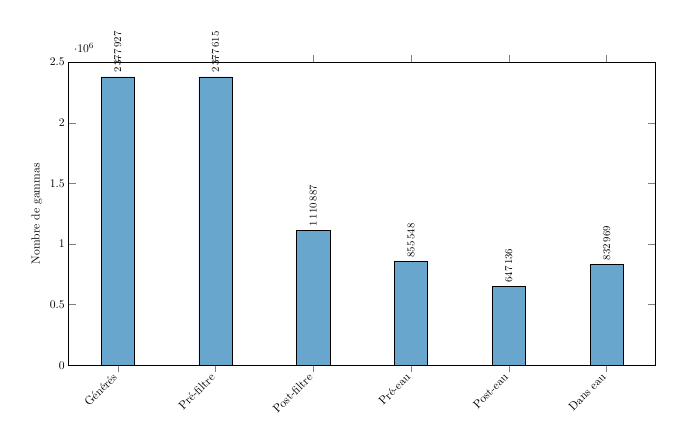
\begin{tikzpicture}[scale=0.6, every node/.style={scale=0.7}]
\begin{axis}[
    ybar,
    width=14cm,
    height=8cm,
    ylabel={Nombre de gammas},
    symbolic x coords={Générés, Pré-filtre, Post-filtre, Pré-eau, Post-eau, Dans eau},
    xtick=data,
    x tick label style={rotate=45, anchor=east},
    ymin=0,
    ymax=2500000,
    bar width=20pt,
    nodes near coords,
    nodes near coords style={font=\small, rotate=90, anchor=west},
    every node near coord/.append style={/pgf/number format/.cd, fixed, precision=0, 1000 sep={\,}},
]
\addplot[fill=headerblue!70] coordinates {
    (Générés, 2377927)
    (Pré-filtre, 2377615)
    (Post-filtre, 1110887)
    (Pré-eau, 855548)
    (Post-eau, 647136)
    (Dans eau, 832969)
};
\end{axis}
\end{tikzpicture}
\captionsetup{labelformat=empty}
\caption{\footnotesize Flux de gammas à travers la géométrie}
\end{figure}

\normalsize
\noindent \color{blue}\textbf{Bilan Quantitatif}\color{black}
\footnotesize
\smallskip

\begin{table}[h!]
\centering
\renewcommand{\arraystretch}{1.3}
\begin{tabular}{|l|r|r|}
\hline
\rowcolor{headerblue}
\footnotesize \textcolor{white}{\textbf{Étape}} &\footnotesize  \textcolor{white}{\textbf{Nombre}} &\footnotesize  \textcolor{white}{\textbf{\% du total généré}} \\
\hline
\footnotesize Gammas générés &\footnotesize  \num{2377927} &\footnotesize  100\% \\
\hline
\footnotesize Atteignent le pré-filtre &\footnotesize  \num{2377615} &\footnotesize  99.99\% \\
\hline
\footnotesize Traversent le filtre (plans) &\footnotesize  \num{1110887} &\footnotesize  46.72\% \\
\hline
\footnotesize Atteignent le pré-eau &\footnotesize  \num{855548} & 35.98\% \\
\hline
\footnotesize Traversent l'eau (plans) &\footnotesize  \num{647136} & 27.21\% \\
\hline
\footnotesize Entrent dans l'eau &\footnotesize  \num{832969} &\footnotesize  35.03\% \\
\hline
\hline
\footnotesize Électrons créés dans l'eau &\footnotesize  \num{5574} &\footnotesize  0.23\% \\
\hline
\end{tabular}
\captionsetup{labelformat=empty}
\caption{\footnotesize Bilan des particules à travers la géométrie}
\end{table}

\normalsize
\noindent \color{blue}\textbf{Pertes Géométriques}\color{black}
\footnotesize
\smallskip

\noindent Entre le post-filtre et le pré-eau :

\begin{equation*}
\text{Pertes} = \num{1110887} - \num{855548} = \num{255339} \quad (23.0\%)
\end{equation*}

\noindent Ces pertes correspondent aux gammas qui :

\begin{itemize}
\item Passent à côté du container (parois latérales)
\item Sont absorbés dans les parois du container
\item Sont diffusés hors de l'acceptance géométrique
\end{itemize}

%===============================================================================
\normalsize
\noindent \begin{mdframed}[backgroundcolor=orange!20]
\subsection{\color{blue}\textbf{Dose dans les Anneaux d'Eau}\color{black}}
\end{mdframed}
\footnotesize
%===============================================================================
\medskip

\normalsize
\noindent \color{blue}\textbf{Résultats par Anneau}\color{black}
\footnotesize
\smallskip

\begin{table}[H]
\centering
\renewcommand{\arraystretch}{1.3}
\begin{tabular}{|c|c|r|r|r|r|}
\hline
\rowcolor{headerblue}
\footnotesize \textcolor{white}{\textbf{Ring}} &\footnotesize  \textcolor{white}{\textbf{Rayon (mm)}} &\footnotesize  \textcolor{white}{\textbf{Énergie (keV)}} &\footnotesize  \textcolor{white}{\textbf{Événements}} &\footnotesize  \textcolor{white}{\textbf{Masse (g)}} &\footnotesize  \textcolor{white}{\textbf{Débit (nGy/h)}} \\
\hline
\footnotesize 0 &\footnotesize  0--5 &\footnotesize  \num{423140} &\footnotesize  \num{1629} &\footnotesize  0.393 &\footnotesize  667.7 \\
\hline
\footnotesize 1 &\footnotesize  5--10 &\footnotesize  \num{1306460} &\footnotesize  \num{5040} &\footnotesize  1.178 &\footnotesize  687.2 \\
\hline
\footnotesize 2 &\footnotesize 10--15 &\footnotesize  \num{2066980} &\footnotesize  \num{8022} &\footnotesize  1.963 &\footnotesize  652.3 \\
\hline
\footnotesize 3 &\footnotesize  15--20 &\footnotesize  \num{2757760} &\footnotesize  \num{10711} &\footnotesize  2.749 &\footnotesize  621.7 \\
\hline
\footnotesize 4 &\footnotesize  20--25 &\footnotesize  \num{3839570} &\footnotesize  \num{14075} &\footnotesize  3.534 &\footnotesize  673.2 \\
\hline
\hline
\textbf{Total} &\footnotesize  0--25 &\footnotesize  \num{10393910} &\footnotesize  \num{39477} &\footnotesize  9.817 &\footnotesize  \textbf{656.1} \\
\hline
\end{tabular}
\captionsetup{labelformat=empty}
\caption{\footnotesize Dose déposée dans chaque anneau d'eau}
\end{table}

\normalsize
\noindent \color{blue}\textbf{Distribution Radiale de la Dose}\color{black}
\footnotesize
\smallskip

\begin{figure}[H]
\centering
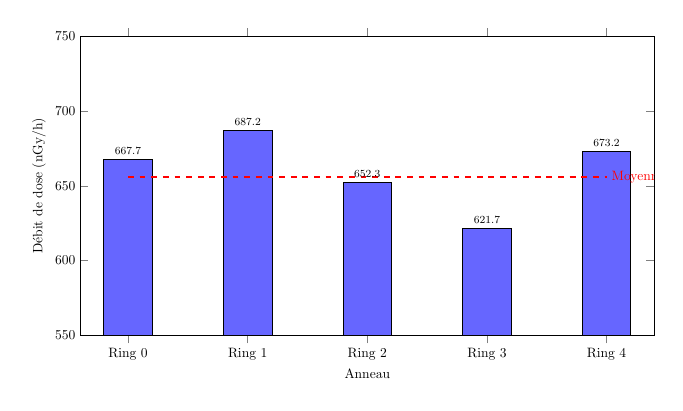
\begin{tikzpicture}[scale=0.7, every node/.style={scale=0.7}]
\begin{axis}[
    ybar,
    width=12cm,
    height=7cm,
    xlabel={Anneau},
    ylabel={Débit de dose (nGy/h)},
    symbolic x coords={Ring 0, Ring 1, Ring 2, Ring 3, Ring 4},
    xtick=data,
    ymin=550,
    ymax=750,
    bar width=25pt,
    nodes near coords,
    nodes near coords style={font=\footnotesize},
]
\addplot[fill=blue!60] coordinates {
    (Ring 0, 667.7)
    (Ring 1, 687.2)
    (Ring 2, 652.3)
    (Ring 3, 621.7)
    (Ring 4, 673.2)
};
\draw[dashed, red, thick] (axis cs:Ring 0,656.1) -- (axis cs:Ring 4,656.1) node[right] {Moyenne};
\end{axis}
\end{tikzpicture}
\captionsetup{labelformat=empty}
\caption{Débit de dose par anneau -- Distribution relativement uniforme}
\end{figure}

\normalsize
\noindent \color{blue}\textbf{Analyse de l'Uniformité}\color{black}
\footnotesize
\smallskip

\noindent Le débit de dose moyen est $\bm{\bar{D}} = \SI{656.1}{\nano\gray\per\hour}$.

\noindent Écart-type des débits de dose :

\begin{equation*}
\bm{\sigma_D} = \sqrt{\frac{\bm{1}}{\bm{5}}\sum_{\bm{i}=\bm{0}}^{\bm{4}}(\bm{D_i} - \bm{\bar{D}})^2} = \SI{24.8}{\nano\gray\per\hour}
\end{equation*}

\noindent Coefficient de variation :

\begin{equation*}
\bm{CV} = \frac{\bm{\sigma_D}}{\bm{\bar{D}}} = \frac{\bm{24.8}}{\bm{656.1}} = \bm{3.8}\%
\end{equation*}

\begin{tcolorbox}[colback=headerblue!10,colframe=headerblue,title=Cohérence Uniformité de la Dose]
\noindent Le coefficient de variation de 3.8\% indique une distribution de dose relativement homogène sur l'ensemble des anneaux. L'écart maximal par rapport à la moyenne est de $\pm$5\%.
\end{tcolorbox}

\normalsize
\noindent \color{blue}\textbf{Proportionnalité Énergie/Aire}\color{black}
\footnotesize
\smallskip

\noindent L'énergie déposée devrait être proportionnelle à l'aire de chaque anneau (pour une irradiation uniforme).

\begin{table}[h!]
\centering
\renewcommand{\arraystretch}{1.3}
\begin{tabular}{|c|c|r|r|r|}
\hline
\rowcolor{headerblue}
\footnotesize \textcolor{white}{\textbf{Ring}} &\footnotesize  \textcolor{white}{\textbf{Aire (mm²)}} &\footnotesize  \textcolor{white}{\textbf{Aire relative}} &\footnotesize  \textcolor{white}{\textbf{Énergie relative}} &\footnotesize  \textcolor{white}{\textbf{Ratio}} \\
\hline
\footnotesize 0 &\footnotesize  $\pi \times 25$ = 78.5 &\footnotesize  1.00 &\footnotesize  1.00 &\footnotesize  1.00 \\
\hline
\footnotesize 1 &\footnotesize  $\pi \times 75$ = 235.6 &\footnotesize  3.00 &\footnotesize  3.09 &\footnotesize  1.03 \\
\hline
\footnotesize 2 &\footnotesize  $\pi \times 125$ = 392.7 &\footnotesize  5.00 &\footnotesize  4.89 &\footnotesize  0.98 \\
\hline
\footnotesize 3 &\footnotesize  $\pi \times 175$ = 549.8 &\footnotesize  7.00 &\footnotesize  6.52 &\footnotesize  0.93 \\
\hline
\footnotesize 4 &\footnotesize  $\pi \times 225$ = 706.9 &\footnotesize  9.00 &\footnotesize  9.08 &\footnotesize  1.01 \\
\hline
\end{tabular}
\captionsetup{labelformat=empty}
\caption{\footnotesize Vérification de la proportionnalité énergie/aire}
\end{table}

\noindent Les ratios proches de 1.0 confirment que l'énergie déposée est bien proportionnelle à l'aire, comme attendu pour une source ponctuelle à incidence normale.

%===============================================================================
\normalsize
\noindent \begin{mdframed}[backgroundcolor=orange!20]
\subsection{\color{blue}\textbf{Renormalisation Temporelle}\color{black}}
\end{mdframed}
\footnotesize
%===============================================================================
\medskip

\normalsize
\noindent \color{blue}\textbf{Paramètres de la Source}\color{black}
\footnotesize
\smallskip

\begin{table}[h!]
\centering
\renewcommand{\arraystretch}{1.3}
\begin{tabular}{|l|r|}
\hline
\rowcolor{headerblue}
\footnotesize \textcolor{white}{\textbf{Paramètre}} &\footnotesize  \textcolor{white}{\textbf{Valeur}} \\
\hline
\footnotesize Activité source ($\bm{4\pi}$) &\footnotesize  \SI{44}{\kilo\becquerel} \\
\hline
\footnotesize Demi-angle du cône $\bm{\theta}$ &\footnotesize  \SI{20}{\degree} \\
\hline
\footnotesize Fraction d'angle solide $\bm{f}$ &\footnotesize  3.015\% \\
\hline
\footnotesize Événements simulés $\bm{N_{\text{sim}}}$ &\footnotesize  \num{1234936} \\
\hline
\end{tabular}
\end{table}

\normalsize
\noindent \color{blue}\textbf{Calcul du Temps d'Irradiation}\color{black}
\footnotesize
\smallskip

\noindent La fraction d'angle solide du cône est :

\begin{equation*}
\bm{f} = \frac{\bm{\Omega}}{\bm{4\pi}} = \frac{\bm{1} - \cos\bm{\theta}}{\bm{2}} = \frac{\bm{1} - \cos(\bm{20}°)}{\bm{2}} = \bm{}0.03015
\end{equation*}

\noindent Le taux de désintégrations dans le cône est :

\begin{equation*}
\bm{\dot{N}_{\text{cône}}} = \bm{f} \times \bm{A} = \bm{0.03015} \times \SI{44000}{\becquerel} = \SI{1327}{\per\second}
\end{equation*}

\noindent Le temps d'irradiation équivalent est :

\begin{equation*}
\bm{T_{\text{irr}}} = \frac{\bm{N_{\text{sim}}}}{\bm{\dot{N}_{\text{cône}}}} = \frac{\num{1234936}}{\SI{1327}{\per\second}} = \SI{930.8}{\second} = \SI{15.51}{\minute}
\end{equation*}

\normalsize
\noindent \color{blue}\textbf{Vérification}\color{black}
\footnotesize
\smallskip

\begin{equation*}
\bm{N_{4\pi,\text{équiv}}} = \frac{\bm{N_{\text{sim}}}}{\bm{f}} = \frac{\num{1234936}}{0.03015} = \num{40954722} \text{ désintégrations}
\end{equation*}

\noindent Durée correspondante pour une source $4\pi$ :

\begin{equation*}
\bm{T} = \frac{\bm{N_{4\pi,\text{équiv}}}}{\bm{A}} = \frac{\num{40954722}}{\SI{44000}{\becquerel}} = \SI{930.8}{\second} \quad \checkmark
\end{equation*}

\begin{tcolorbox}[colback=headerblue!10,colframe=headerblue,title=Cohérence Renormalisation]
\noindent Le temps d'irradiation de \SI{15.5}{\minute} correspond bien à \num{1.23} millions de désintégrations dans un cône de \SI{20}{\degree} pour une source de \SI{44}{\kilo\becquerel}.
\end{tcolorbox}

%===============================================================================
\normalsize
\noindent \begin{mdframed}[backgroundcolor=orange!20]
\subsection{\color{blue}\textbf{Vérification de la Cohérence Globale}\color{black}}
\end{mdframed}
\footnotesize
%===============================================================================
\medskip

\normalsize
\noindent \color{blue}\textbf{Tableau Récapitulatif}\color{black}
\footnotesize
\smallskip

\begin{table}[h!]
\centering
\renewcommand{\arraystretch}{1.4}
\begin{tabular}{|p{5cm}|c|c|c|}
\hline
\rowcolor{headerblue}
\footnotesize \textcolor{white}{\textbf{Test}}&\footnotesize \textcolor{white}{\textbf{Attendu}}&\footnotesize \textcolor{white}{\textbf{Mesuré}}&\footnotesize \textcolor{white}{\textbf{Statut}}\\
\hline
\footnotesize Gammas/événement&\footnotesize 1.924&\footnotesize 1.926&\footnotesize \cellcolor{okgreen!30}$\checkmark$\\
\hline
\footnotesize Transmission filtre W/PETG&\footnotesize 45--50\%&\footnotesize 47\%&\footnotesize \cellcolor{okgreen!30}$\checkmark$ \\
\hline
\footnotesize Transmission eau 5 mm&\footnotesize 70--80\%&\footnotesize 76\%&\footnotesize \cellcolor{okgreen!30}$\checkmark$ \\
\hline
\footnotesize Uniformité dose (CV)&\footnotesize $<$10\%&\footnotesize 3.8\%&\footnotesize \cellcolor{okgreen!30}$\checkmark$ \\
\hline
\footnotesize Proportionnalité E/Aire&\footnotesize $\sim$1.0&\footnotesize 0.93--1.03&\footnotesize \cellcolor{okgreen!30}$\checkmark$ \\
\hline
\footnotesize Cohérence plans/entrée&\footnotesize $<$5\%&\footnotesize 0.7\%&\footnotesize \cellcolor{okgreen!30}$\checkmark$ \\
\hline
\end{tabular}
\captionsetup{labelformat=empty}
\caption{\footnotesize Récapitulatif des tests de cohérence}
\end{table}

\normalsize
\noindent \color{blue}\textbf{Incertitudes Statistiques}\color{black}
\footnotesize
\smallskip

\noindent Pour $\bm{N} = \num{1234936}$ événements, l'incertitude statistique relative est :

\begin{equation*}
\frac{\bm{\sigma}}{\bm{\mu}} \approx \frac{\bm{1}}{\sqrt{\bm{N}}} = \frac{\bm{1}}{\sqrt{\num{1234936}}} = \bm{0.09}\%
\end{equation*}

\noindent Les incertitudes sur les compteurs sont :
\begin{itemize}
\item Transmission filtre : $47.44\% \pm 0.04\%$
\item Transmission eau : $75.64\% \pm 0.08\%$
\item Débit de dose : $656 \pm 1$ nGy/h
\end{itemize}


\clearpage

%==============================================================================
\normalsize
\noindent \begin{mdframed}[backgroundcolor=orange!20]
\section{\Large \color{blue} \textbf{Résultats principaux}\color{black}}
\end{mdframed}
\footnotesize
%==============================================================================


%===============================================================================
\normalsize
\noindent \begin{mdframed}[backgroundcolor=orange!20]
\subsection{\color{blue}\textbf{Bilan des gammas}\color{black}}
\end{mdframed}
\footnotesize
%===============================================================================
\medskip

\normalsize
\noindent \color{blue}\textbf{bilan des désintégrations}\color{black}
\footnotesize
\smallskip


\begin{table}[h!]
\centering
\captionsetup{labelformat=empty}
\caption{\footnotesize Bilan des photons gamma pour $10^6$ désintégrations.}
\begin{tabular}{lrr}
\toprule
\footnotesize \textbf{Catégorie} &\footnotesize  \textbf{Nombre} &\footnotesize  \textbf{Fraction (\%)} \\
\midrule
\footnotesize Primaires générés &\footnotesize  1\,443\,552 &\footnotesize  100.0 \\
\footnotesize Absorbés dans le filtre &\footnotesize  434\,560 &\footnotesize  30.1 \\
\footnotesize Transmis (sortis du filtre) &\footnotesize  1\,010\,078 &\footnotesize  69.9 \\
\footnotesize Entrés dans l'eau &\footnotesize  732\,707 &\footnotesize  50.8 \\
\footnotesize Absorbés dans l'eau &\footnotesize  17 &\footnotesize  0.002 \\
\bottomrule
\end{tabular}
\end{table}

\noindent Le nombre moyen de gammas par désintégration est $\bar{n}_\gamma = 1.44$, conforme à la valeur théorique de 1.44 pour l'$^{152}$Eu (somme des intensités des 11 raies principales).

\medskip
\normalsize
\noindent \color{blue}\textbf{Taux d'absorption par raie gamma}\color{black}
\footnotesize
\medskip

\noindent Le tableau~suivant présente les taux d'absorption dans le filtre $\bm{W/PETG}$ pour chaque raie gamma de l'$^{152}$Eu.

\begin{table}[h!]
\centering
\captionsetup{labelformat=empty}
\caption{\footnotesize Taux d'absorption des raies gamma de l'$^{152}$Eu dans le filtre $\bm{W/PETG}$ (75\%/25\%) d'épaisseur 5~mm. Simulation Geant4 avec $10^6$ désintégrations.}
\begin{tabular}{cccccc}
\toprule
\footnotesize \textbf{Énergie}&\footnotesize \textbf{Intensité}&\footnotesize \textbf{Émis}&\footnotesize \textbf{Absorbés}&\footnotesize  \textbf{Transmis}&\footnotesize \textbf{Taux d'absorption} \\
\textbf{(keV)} &\footnotesize  \textbf{(\%)} & &\footnotesize \textbf{(filtre)}&\footnotesize \textbf{(filtre)}&\footnotesize  \textbf{(\%)} \\
\midrule
\footnotesize 121.78&\footnotesize 28.4&\footnotesize 284\,132&\footnotesize 278\,622&\footnotesize 5\,520&\footnotesize $98.06\pm 0.03$\\
\footnotesize 244.70&\footnotesize 7.5 &\footnotesize 75\,251&\footnotesize 38\,758&\footnotesize 36\,570&\footnotesize $51.50\pm0.18$\\
\footnotesize 344.28&\footnotesize 26.5&\footnotesize 265\,450&\footnotesize 74\,040&\footnotesize 191\,783&\footnotesize $27.89\pm0.09$\\
\footnotesize 411.12&\footnotesize 2.2&\footnotesize 22\,369&\footnotesize 4\,581&\footnotesize 17\,823&\footnotesize $20.48 \pm 0.27$ \\
\footnotesize 443.97&\footnotesize 2.8&\footnotesize 28\,541&\footnotesize 4\,954&\footnotesize 23\,623&\footnotesize $17.36 \pm 0.22$ \\
\footnotesize 778.90&\footnotesize 12.9&\footnotesize 129\,290&\footnotesize 8\,713&\footnotesize 120\,697&\footnotesize $6.74\pm0.07$ \\
\footnotesize 867.38&\footnotesize 4.2&\footnotesize 42\,550&\footnotesize 2\,371&\footnotesize 40\,212&\footnotesize  $5.57 \pm 0.11$ \\
\footnotesize 964.08&\footnotesize 14.6&\footnotesize 146\,493&\footnotesize 6\,992&\footnotesize 139\,620&\footnotesize $4.77\pm0.06$ \\
\footnotesize 1085.8&\footnotesize 10.2&\footnotesize 102\,060&\footnotesize 4\,133&\footnotesize 97\,999&\footnotesize $4.05\pm0.06$ \\
\footnotesize 1112.0&\footnotesize 13.6&\footnotesize 136\,706&\footnotesize 5\,177&\footnotesize 131\,631&\footnotesize $3.79\pm0.05$ \\
\footnotesize 1408.0&\footnotesize 21.0&\footnotesize 210\,710&\footnotesize 6\,219&\footnotesize 204\,600&\footnotesize $2.95\pm0.04$ \\
\midrule
\footnotesize \textbf{Total}&\footnotesize \textbf{143.9}&\footnotesize \textbf{1\,443\,552}&\footnotesize \textbf{434\,560}&\footnotesize  \textbf{1\,010\,078} &\footnotesize  $\mathbf{30.10 \pm 0.04}$ \\
\bottomrule
\end{tabular}
\end{table}

\begin{table}[h!]
\centering
\captionsetup{labelformat=empty}
\caption{\footnotesize Taux d'absorption des raies $\gamma$ de l'$^{152}$Eu dans 5~mm de $\bm{W/PETG}$ (75\%/25\%).}
\begin{tabular}{cc|cc}
\toprule
\footnotesize \textbf{$E_\gamma$ (keV)}&\footnotesize \textbf{Absorption (\%)}&\footnotesize \textbf{$E_\gamma$ (keV)}& \footnotesize\textbf{Absorption (\%)} \\
\midrule
\footnotesize 121.78&\footnotesize $98.06 \pm 0.03$&\footnotesize 867.38&\footnotesize $5.57 \pm 0.11$ \\
\footnotesize 244.70&\footnotesize $51.50 \pm 0.18$&\footnotesize 964.08&\footnotesize $4.77 \pm 0.06$ \\
\footnotesize 344.28&\footnotesize $27.89 \pm 0.09$&\footnotesize 1085.87&\footnotesize $4.05 \pm 0.06$ \\
\footnotesize 411.12&\footnotesize $20.48 \pm 0.27$&\footnotesize 1112.07&\footnotesize $3.79 \pm 0.05$ \\
\footnotesize 443.97&\footnotesize $17.36 \pm 0.22$&\footnotesize 1408.01&\footnotesize $2.95 \pm 0.04$ \\
\footnotesize 778.90&\footnotesize $6.74 \pm 0.07$ & & \\
\bottomrule
\end{tabular}
\end{table}

\newpage

%===============================================================================
\normalsize
\noindent \begin{mdframed}[backgroundcolor=orange!20]
\subsection{\color{blue}\textbf{Calcul des doses déposées avec le filtre W/PETG de 5mm}\color{black}}
\end{mdframed}
\footnotesize
%===============================================================================
\medskip

\begin{table}[h!]
\centering
\captionsetup{labelformat=empty}
\caption{\footnotesize Dose déposée par anneau d'eau pour $10^6$ désintégrations d'$^{152}$Eu. Épaisseur d'eau: 5~mm, largeur radiale des anneaux: 5~mm.}
\begin{tabular}{ccccccc}
\toprule
\footnotesize \textbf{Anneau} &\footnotesize $\bm{r_{in}}$&\footnotesize $\bm{r_{out}}$&\footnotesize \textbf{Masse}&\footnotesize $\bm{E_{dep}}$&\footnotesize \textbf{Dose}&\footnotesize \textbf{Dose/désint.} \\
 &\footnotesize  \textbf{(mm)}&\footnotesize \textbf{(mm)}&\footnotesize \textbf{(g)}&\footnotesize \textbf{(MeV)}&\footnotesize  \textbf{(nGy)}&\footnotesize \textbf{(nGy)} \\
\midrule
\footnotesize 0&\footnotesize 0&\footnotesize 5 &\footnotesize 0.393&\footnotesize $3.91\times10^2$&\footnotesize  159.7 & $1.09 \times 10^{-1}$ \\
\footnotesize 1&\footnotesize 5&\footnotesize 10&\footnotesize 1.178&\footnotesize $1.14\times10^3$&\footnotesize 155.0&\footnotesize  $3.61 \times 10^{-2}$ \\
\footnotesize 2&\footnotesize 10&\footnotesize 15&\footnotesize 1.964&\footnotesize $1.86\times10^3$&\footnotesize 151.5&\footnotesize  $2.17 \times 10^{-2}$\\
\footnotesize 3&\footnotesize 15&\footnotesize 20&\footnotesize 2.749&\footnotesize $2.50\times10^3$&\footnotesize 145.9&\footnotesize  $1.54 \times 10^{-2}$\\
\footnotesize 4&\footnotesize 20&\footnotesize 25&\footnotesize 3.534&\footnotesize $3.44\times10^3$ 156.0&\footnotesize $1.29 \times 10^{-2}$ \\
\midrule
\footnotesize \textbf{Total}&\footnotesize 0&\footnotesize 25&\footnotesize \textbf{9.818}&\footnotesize $\mathbf{9.33 \times 10^3}$&\footnotesize \textbf{152.3} & $\mathbf{1.52 \times 10^{-4}}$ \\
\bottomrule
\end{tabular}
\end{table}

\normalsize
\noindent \color{blue}\textbf{Dose déposée par anneau}\color{black}
\footnotesize
\smallskip

\begin{figure}[h!]
    \centering
    \includegraphics[scale=0.6]{Figures/dose_par_anneau_FiltreWPETG_5mm.png}
		\captionsetup{labelformat=empty}
    \caption{Distribution de la dose par anneau d'eau avec un filtre de $\bm{W/PETG}$ de 5 mm.}
\end{figure}

\normalsize
\noindent \color{blue}\textbf{Taux d'absorption par raie gamma}\color{black}
\footnotesize
\smallskip

\begin{figure}[h!]
    \centering
    \includegraphics[scale=0.5]{Figures/taux_absorption_FiltreWPETG_5mm.png}
		\captionsetup{labelformat=empty}
    \caption{Absorption du filtre de $\bm{W/PETG}$ de 5mm}
\end{figure}

\newpage

%==============================================================================
\normalsize
\noindent \begin{mdframed}[backgroundcolor=orange!20]
\section{\Large \color{blue} \textbf{Ajout de plan de comptage avant et aprés le container d'eau}\color{black}}
\end{mdframed}
\footnotesize
%==============================================================================

\begin{tcolorbox}[colback=blue!5,colframe=blue,title=\textbf{Changement de géométrie}]
\noindent Le container d'eau est précédé et suivi de deux plans de comptage, de 1 mm d'epaisser. L'objectif de ces plan de comptage est de caractériser la production d'électrons secondaires
\end{tcolorbox}

%===============================================================================
\normalsize
\noindent \begin{mdframed}[backgroundcolor=orange!20]
\subsection{\color{blue}\textbf{Vue en coupe de la géométrie}\color{black}}
\end{mdframed}
\footnotesize
%===============================================================================
\medskip

\noindent La figure suivante présente une vue en coupe axiale (plan XZ) de la géométrie du container et des plans de comptage associés.

\begin{figure}[h!]
\centering
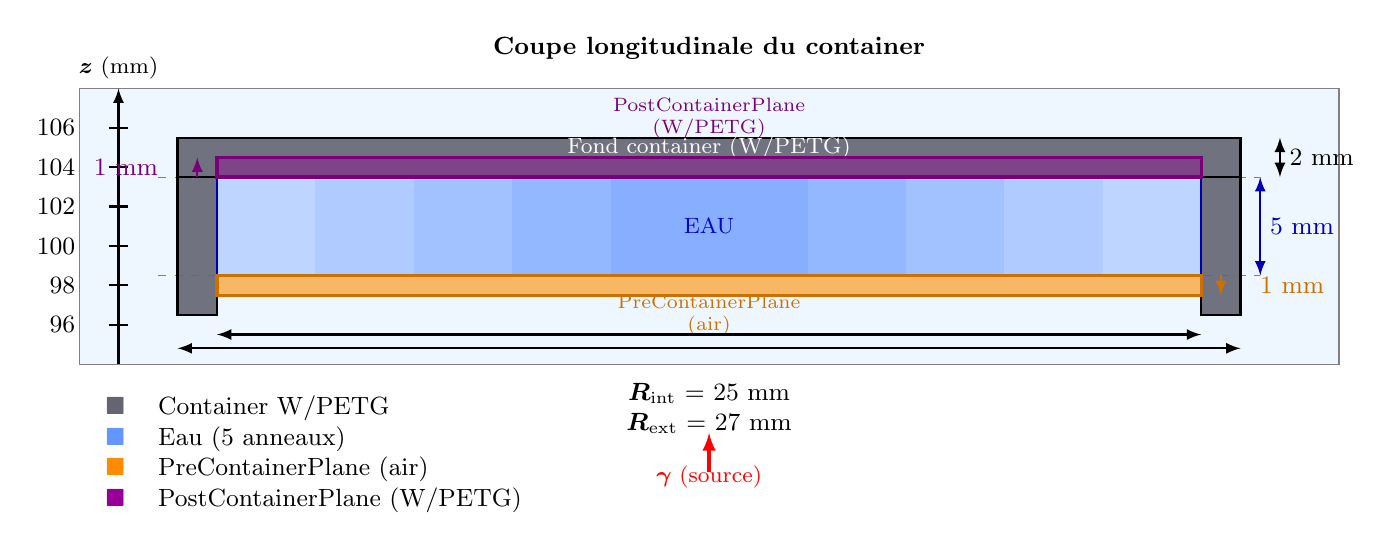
\begin{tikzpicture}[scale=0.25, >=latex]
    
    % ═══════════════════════════════════════════════════════════════
    % ÉCHELLE : 1 unité = 1 mm (échelle x0.5)
    % Vue en coupe longitudinale (plan XZ) - Container uniquement
    % Agrandissement : z de 94 mm à 108 mm, x de -32 mm à 32 mm
    % ═══════════════════════════════════════════════════════════════
    
    % Cadre et fond (air)
    \fill[aircolor, opacity=0.3] (-32,94) rectangle (32,108);
    \draw[gray, thin] (-32,94) rectangle (32,108);
    
    % ═══════════════════════════════════════════════════════════════
    % AXE DES Z (vertical) avec graduations
    % ═══════════════════════════════════════════════════════════════
    \draw[->, thick] (-30,94) -- (-30,108);
    \node[above, font=\footnotesize] at (-30,108) {$\bm{z}$ (mm)};
    
    \foreach \z in {96,98,100,102,104,106} {
        \draw[thick] (-30.5,\z) -- (-29.5,\z);
        \node[left, font=\small] at (-31.7,\z) {\z};
    }
    
    % Lignes de référence horizontales (pointillées)
    \foreach \z in {98.5, 103.5} {
        \draw[gray, dashed, thin] (-28,\z) -- (28,\z);
    }
    
    % ═══════════════════════════════════════════════════════════════
    % CONTAINER - Parois latérales (W/PETG)
    % Rayon intérieur = 25 mm, extérieur = 27 mm
    % z de 96.5 à 103.5 mm (ouvert en bas, fermé en haut)
    % ═══════════════════════════════════════════════════════════════
    
    % Paroi gauche
    \fill[containercolor, opacity=0.9] (-27,96.5) rectangle (-25,103.5);
    \draw[black, thick] (-27,96.5) rectangle (-25,103.5);
    
    % Paroi droite
    \fill[containercolor, opacity=0.9] (25,96.5) rectangle (27,103.5);
    \draw[black, thick] (25,96.5) rectangle (27,103.5);
    
    % ═══════════════════════════════════════════════════════════════
    % CONTAINER - Fond (W/PETG)
    % z de 103.5 à 105.5 mm, rayon = 27 mm
    % ═══════════════════════════════════════════════════════════════
    
    \fill[containercolor, opacity=0.9] (-27,103.5) rectangle (27,105.5);
    \draw[black, thick] (-27,103.5) rectangle (27,105.5);
    \node[font=\footnotesize, white] at (0,105) {Fond container (W/PETG)};
    
    % ═══════════════════════════════════════════════════════════════
    % EAU - 5 anneaux concentriques (en coupe)
    % z de 98.5 à 103.5 mm (5 mm épaisseur)
    % Anneaux de 5 mm de largeur chacun
    % ═══════════════════════════════════════════════════════════════
    
    % Anneau 4 (externe) : r = 20-25 mm
    \fill[watercolor, opacity=0.35] (-25,98.5) rectangle (-20,103.5);
    \fill[watercolor, opacity=0.35] (20,98.5) rectangle (25,103.5);
    
    % Anneau 3 : r = 15-20 mm
    \fill[watercolor, opacity=0.45] (-20,98.5) rectangle (-15,103.5);
    \fill[watercolor, opacity=0.45] (15,98.5) rectangle (20,103.5);
    
    % Anneau 2 : r = 10-15 mm
    \fill[watercolor, opacity=0.55] (-15,98.5) rectangle (-10,103.5);
    \fill[watercolor, opacity=0.55] (10,98.5) rectangle (15,103.5);
    
    % Anneau 1 : r = 5-10 mm
    \fill[watercolor, opacity=0.65] (-10,98.5) rectangle (-5,103.5);
    \fill[watercolor, opacity=0.65] (5,98.5) rectangle (10,103.5);
    
    % Anneau 0 (central) : r = 0-5 mm
    \fill[watercolor, opacity=0.75] (-5,98.5) rectangle (5,103.5);
    
    % Contour eau
    \draw[blue!70!black, thick] (-25,98.5) rectangle (25,103.5);
    \node[font=\footnotesize, blue!80!black] at (0,101) {EAU};
    
    % ═══════════════════════════════════════════════════════════════
    % PLAN PRE-CONTAINER (Orange, Air)
    % z centre = 98.0 mm, épaisseur = 1 mm
    % Limite haute = 98.5 mm (bas de l'eau) - GAP=0
    % ═══════════════════════════════════════════════════════════════
    
    \fill[precontainercolor, opacity=0.6] (-25,97.5) rectangle (25,98.5);
    \draw[precontainercolor!80!black, very thick] (-25,97.5) rectangle (25,98.5);
    \node[font=\scriptsize, precontainercolor!80!black, align=center] at (0,96.5) 
        {PreContainerPlane\\(air)};
    
    % Flèche indiquant la limite
    \draw[precontainercolor!80!black, thick, ->] (26,98.5) -- (26,97.5);
    \node[right, font=\small, precontainercolor!80!black] at (27.5,98) {1 mm};
    
    % ═══════════════════════════════════════════════════════════════
    % PLAN POST-CONTAINER (Violet, W/PETG)
    % z centre = 104.0 mm, épaisseur = 1 mm
    % Limite basse = 103.5 mm (haut de l'eau) - GAP=0
    % ═══════════════════════════════════════════════════════════════
    
    \fill[postcontainercolor, opacity=0.4] (-25,103.5) rectangle (25,104.5);
    \draw[postcontainercolor!80!black, very thick] (-25,103.5) rectangle (25,104.5);
    \node[font=\scriptsize, postcontainercolor!80!black, align=center] at (0,106.5) 
        {PostContainerPlane\\(W/PETG)};
    
    % Flèche indiquant la limite
    \draw[postcontainercolor!80!black, thick, ->] (-26,103.5) -- (-26,104.5);
    \node[left, font=\small, postcontainercolor!80!black] at (-27.5,104) {1 mm};
    
    % ═══════════════════════════════════════════════════════════════
    % COTES ET ANNOTATIONS
    % ═══════════════════════════════════════════════════════════════
    
    % Cote épaisseur eau
    \draw[<->, blue!70!black, thick] (28,98.5) -- (28,103.5);
    \node[right, font=\small, blue!70!black] at (28,101) {5 mm};
    
    % Cote épaisseur fond container
    \draw[<->, black, thick] (29,103.5) -- (29,105.5);
    \node[right, font=\small] at (29,104.5) {2 mm};
    
    % Cote rayon eau/container
    \draw[<->, thick] (-25,95.5) -- (25,95.5);
    \node[below, font=\small] at (0,93.5) {$\bm{R_{\text{int}}}$ = 25 mm};
    
    % Cote rayon externe
    \draw[<->, thick] (-27,94.8) -- (27,94.8);
    \node[below, font=\small] at (0,92) {$\bm{R_{\text{ext}}}$ = 27 mm};
    
    % ═══════════════════════════════════════════════════════════════
    % FLÈCHE DIRECTION SOURCE (bas)
    % ═══════════════════════════════════════════════════════════════
    
    \draw[->, red, very thick] (0,88.5) -- (0,90.5);
    \node[below, font=\footnotesize, red] at (0,89.3) {$\bm{\gamma}$ (source)};
    
    % ═══════════════════════════════════════════════════════════════
    % LÉGENDE
    % ═══════════════════════════════════════════════════════════════
    
    \node[font=\small, anchor=north west] at (-32,93) {
        \begin{tabular}{ll}
            \textcolor{containercolor}{$\blacksquare$} & Container W/PETG \\
            \textcolor{watercolor}{$\blacksquare$} & Eau (5 anneaux) \\
            \textcolor{precontainercolor}{$\blacksquare$} & PreContainerPlane (air) \\
            \textcolor{postcontainercolor}{$\blacksquare$} & PostContainerPlane (W/PETG) \\
        \end{tabular}
    };
    
    % ═══════════════════════════════════════════════════════════════
    % TITRE
    % ═══════════════════════════════════════════════════════════════
    
    \node[font=\small\bfseries, anchor=south] at (0,109) {Coupe longitudinale du container};
    %\node[font=\footnotesize, anchor=north] at (0,108.5) {(plan XZ, échelle $\times$0.5)};
    
\end{tikzpicture}
		\captionsetup{labelformat=empty}
    \caption{\footnotesize Vue en coupe axiale (plan XZ) du container et des plans de comptage. Les plans de comptage sont représentés avec leur couleur respective : PreContainer (orange) et PostContainer (violet). L'eau est divisée en 5 anneaux concentriques de 5~mm de largeur.}
\end{figure}

%===============================================================================
\normalsize
\noindent \begin{mdframed}[backgroundcolor=orange!20]
\subsection{\color{blue}\textbf{Positions axiales des éléments de la géométrie}\color{black}}
\end{mdframed}
\footnotesize
%===============================================================================
\medskip

\noindent Le tableau suivant récapitule les positions en $\bm{z}$ de tous les éléments de la géométrie.

\begin{table}[h]
\centering
\captionsetup{labelformat=empty}		
\caption{\footnotesize Positions axiales (z) des éléments de la géométrie -- Version actualisée}
\begin{tabular}{llcccc}
\toprule
\footnotesize \textbf{Élément}&\footnotesize \textbf{Matériau}&\footnotesize \textbf{z min (mm)}&\footnotesize \textbf{z centre (mm)}& \textbf{z max (mm)}&\footnotesize \textbf{Rayon (mm)} \\
\midrule
\footnotesize Source Eu-152&\footnotesize --&\footnotesize --&\footnotesize 20.0& --&\footnotesize ponctuelle\\
\midrule
\multicolumn{6}{c}{\footnotesize \textit{Zone filtre}} \\
\midrule
\rowcolor{prefiltercolor!20}
\footnotesize PreFilterPlane &\footnotesize  Air &\footnotesize  35.5 &\footnotesize  36.0 &\footnotesize  36.5 &\footnotesize  25\\
\rowcolor{filtercolor!20}
\footnotesize Filtre W/PETG&\footnotesize W/PETG 75\%/25\%&\footnotesize 37.5&\footnotesize 40.0&\footnotesize 42.5&\footnotesize 25 \\
\rowcolor{postfiltercolor!20}
\footnotesize PostFilterPlane&\footnotesize Air&\footnotesize 43.5&\footnotesize 44.0&\footnotesize 44.5&\footnotesize 25 \\
\midrule
\multicolumn{6}{c}{\footnotesize \textit{Zone container}} \\
\midrule
\footnotesize Container (ouverture)&\footnotesize --&\multicolumn{3}{c}{\footnotesize z = 96.5 (face ouverte)}&\footnotesize 25 (int) / 27 (ext)\\
\rowcolor{precontainercolor!30}
\footnotesize \textbf{PreContainerPlane}&\footnotesize \textbf{Air}&\footnotesize \textbf{97.5}&\footnotesize \textbf{98.0}&\footnotesize  \textbf{98.5}&\footnotesize  \textbf{25} \\
\rowcolor{watercolor!20}
\footnotesize Eau (5 anneaux)&\footnotesize H$_2$O&\footnotesize 98.5&\footnotesize 101.0&\footnotesize 103.5&\footnotesize 25\\
\rowcolor{postcontainercolor!30}
\footnotesize \textbf{PostContainerPlane}&\footnotesize \textbf{W/PETG}&\footnotesize \textbf{103.5}&\footnotesize \textbf{104.0}&\footnotesize  \textbf{104.5}&\footnotesize  \textbf{25} \\
\rowcolor{containercolor!20}
\footnotesize Container (parois)&\footnotesize W/PETG&\footnotesize 96.5&\footnotesize 100.0&\footnotesize 103.5&\footnotesize  25-27 \\
\rowcolor{containercolor!20}
\footnotesize Container (fond)&\footnotesize \footnotesize W/PETG&\footnotesize 103.5 &\footnotesize 104.5&\footnotesize 105.5&\footnotesize  0-27 \\
\bottomrule
\end{tabular}
\end{table}

%===============================================================================
\normalsize
\noindent \begin{mdframed}[backgroundcolor=orange!20]
\subsection{\color{blue}\textbf{Caractéristiques des plans de comptage}\color{black}}
\end{mdframed}
\footnotesize
%===============================================================================
\medskip

\begin{table}[h]
\centering
\caption{\footnotesize Plans de comptage -- Configuration actuelle}
\begin{tabular}{lccccl}
\toprule
\footnotesize \textbf{Plan}&\footnotesize \textbf{z centre}&\footnotesize \textbf{GAP}&\footnotesize \textbf{Épaisseur}&\footnotesize  \textbf{Matériau}&\footnotesize \textbf{Volume logique} \\
&\footnotesize \textbf{(mm)}&\footnotesize \textbf{(mm)}&\footnotesize \textbf{(mm)}& & \\
\midrule
\rowcolor{prefiltercolor!20}
\footnotesize PreFilterPlane&\footnotesize 36.0&\footnotesize 1.0&\footnotesize 1.0&\footnotesize Air& PreFilterPlaneLog \\
\rowcolor{postfiltercolor!20}
\footnotesize PostFilterPlane&\footnotesize 44.0&\footnotesize 1.0 &\footnotesize 1.0&\footnotesize  Air&\footnotesize PostFilterPlaneLog \\
\midrule
\rowcolor{precontainercolor!30}
\footnotesize \textbf{PreContainerPlane}&\footnotesize \textbf{98.0}&\footnotesize \textbf{0}&\footnotesize \textbf{1.0}&\footnotesize  \textbf{Air}&\footnotesize \textbf{PreContainerPlaneLog} \\
\rowcolor{postcontainercolor!30}
\footnotesize \textbf{PostContainerPlane}&\footnotesize \textbf{104.0}&\footnotesize \textbf{0}&\footnotesize \textbf{1.0}&\footnotesize  \textbf{W/PETG}&\footnotesize  \textbf{PostContainerPlaneLog} \\
\bottomrule
\end{tabular}
\end{table}

\vspace{0.5cm}

\begin{tcolorbox}[colback=blue!5,colframe=blue,title=\textbf{Notes}]
\begin{itemize}
\item \textbf{PreContainerPlane} : limite haute (z=98.5 mm) = limite basse de l'eau
\item \textbf{PostContainerPlane} : limite basse (z=103.5 mm) = limite haute de l'eau
\item Les deux plans autour de l'eau ont un GAP = 0 (collés à l'eau)
\item PostContainerPlane est en W/PETG (même matériau que le container)
\end{itemize}
\end{tcolorbox}

%===============================================================================
\normalsize
\noindent \begin{mdframed}[backgroundcolor=orange!20]
\subsection{\color{blue}\textbf{Nouveaux Ntuples : PreContainer et PostContainer}\color{black}}
\end{mdframed}
\footnotesize
%===============================================================================
\medskip

\begin{tcolorbox}[colback=blue!5,colframe=blue,title=\textbf{Addition de ntuple}]
\noindent Deux nouveaux ntuples ont été ajoutés pour enregistrer les passages de particules aux plans de comptage situés juste avant et juste après l'eau (GAP = 0). Les données sont enregistrées \textbf{par désintégration} (un événement = une désintégration).
\end{tcolorbox}
\medskip
\normalsize
\noindent \color{blue}\textbf{Ntuple \textbf{precontainer} (index 2)}\color{black}
\footnotesize
\smallskip

\noindent Ce ntuple enregistre les \textbf{photons} et les \textbf{électrons} traversant le plan PreContainerPlane en direction de l'eau.

\begin{tcolorbox}[colback=headerblue!10,colframe=headerblue!80!black,title=\textbf{Caractéristiques du plan PreContainerPlane}]
\begin{itemize}
    \item \textbf{Position} : z = 97.5 -- 98.5 mm (centre à 98.0 mm)
    \item \textbf{Limite haute} : 98.5 mm = surface basse de l'eau
    \item \textbf{Matériau} : Air
    \item \textbf{GAP} : 0 (collé à l'eau)
    \item \textbf{Rayon} : 25 mm
    \item \textbf{Volume logique} : \texttt{PreContainerPlaneLog}
\end{itemize}
\end{tcolorbox}

\begin{table}[h]
\centering
\captionsetup{labelformat=empty}
\caption{\footnotesize Variables du ntuple \textbf{precontainer}}
\begin{tabular}{llp{8cm}}
\toprule
\footnotesize \textbf{Variable}&\footnotesize \textbf{Type}&\footnotesize \textbf{Description}\\
\midrule
\footnotesize \texttt{nPhotons}&\footnotesize Int&\footnotesize Nombre de photons traversant le plan en direction +z (vers l'eau) \\
\footnotesize \texttt{sumEPhotons\_keV}&\footnotesize Double&\footnotesize Somme des énergies cinétiques de ces photons (keV) \\
\midrule
\footnotesize \texttt{nElectrons}&\footnotesize Int&\footnotesize Nombre d'électrons traversant le plan en direction +z (vers l'eau) \\
\footnotesize \texttt{sumEElectrons\_keV}&\footnotesize Double&\footnotesize  Somme des énergies cinétiques de ces électrons (keV) \\
\bottomrule
\end{tabular}
\end{table}

\medskip
\normalsize
\noindent \color{blue}\textbf{Conditions de remplissage du ntuple \textbf{precontainer}}\color{black}
\footnotesize
\smallskip

\noindent Pour chaque particule traversant le plan \color{blue}\textbf{PreContainerPlane}\color{black} :

\noindent \textbf{Photons vers l'eau}\par
\medskip
\begin{itemize}
\item \textbf{Type de particule} : gamma ($\gamma$)
\item \textbf{Direction} : $p_z > 0$ (vers l'eau, direction +z)
\item \textbf{Condition de passage} : 
\begin{itemize}
\item Volume de départ $\neq$ \texttt{PreContainerPlaneLog}
\item Volume d'arrivée $=$ \texttt{PreContainerPlaneLog}
\end{itemize}
\end{itemize}

\begin{verbatim}
if (postLogVolName == "PreContainerPlaneLog" 
    && logicalVolumeName != "PreContainerPlaneLog") {
    if (particleName == "gamma" && pz > 0) {
        fEventAction->RecordPreContainerPhoton(kineticEnergy);
    }
}
\end{verbatim}


\noindent \textbf{Électrons vers l'eau}\par
\medskip

\begin{itemize}
\item \textbf{Type de particule} : électron ($e^-$)
\item \textbf{Direction} : $p_z > 0$ (vers l'eau, direction +z)
\item \textbf{Condition de passage} : 
\begin{itemize}
\item Volume de départ $\neq$ \texttt{PreContainerPlaneLog}
\item Volume d'arrivée $=$ \texttt{PreContainerPlaneLog}
\end{itemize}
\end{itemize}

\begin{verbatim}
if (postLogVolName == "PreContainerPlaneLog" 
    && logicalVolumeName != "PreContainerPlaneLog") {
    if (particleName == "e-" && pz > 0) {
        fEventAction->RecordPreContainerElectron(kineticEnergy);
    }
}
\end{verbatim}
\medskip
\normalsize
\noindent \color{blue}\textbf{Ntuple \textbf{postcontainer} (index 3)}\color{black}
\footnotesize
\smallskip

\noindent Ce ntuple enregistre les particules traversant le plan PostContainerPlane, avec distinction selon leur type et direction.

\begin{tcolorbox}[colback=headerblue!10,colframe=headerblue!80!black,title=\textbf{Caractéristiques du plan PostContainerPlane}]
\begin{itemize}
    \item \textbf{Position} : z = 103.5 -- 104.5 mm (centre à 104.0 mm)
    \item \textbf{Limite basse} : 103.5 mm = surface haute de l'eau
    \item \textbf{Matériau} : W/PETG (75\%/25\%)
    \item \textbf{GAP} : 0 (collé à l'eau)
    \item \textbf{Rayon} : 25 mm
    \item \textbf{Volume logique} : \texttt{PostContainerPlaneLog}
\end{itemize}
\end{tcolorbox}

\begin{table}[h]
\centering
\captionsetup{labelformat=empty}
\caption{\footnotesize Variables du ntuple \textbf{postcontainer}}
\begin{tabular}{llp{7cm}}
\toprule
\footnotesize \textbf{Variable}&\footnotesize \textbf{Type}&\footnotesize \textbf{Description} \\
\midrule
\footnotesize \texttt{nPhotons\_back}&\footnotesize Int&\footnotesize Nombre de photons venant de l'eau (direction -z) \\
\footnotesize \texttt{sumEPhotons\_back\_keV}&\footnotesize Double&\footnotesize Somme des énergies cinétiques de ces photons (keV) \\
\midrule
\footnotesize \texttt{nElectrons\_back}&\footnotesize Int&\footnotesize  Nombre d'électrons venant de l'eau (direction -z) \\
\footnotesize \texttt{sumEElectrons\_back\_keV}& Double&\footnotesize Somme des énergies cinétiques de ces électrons (keV) \\
\midrule
\footnotesize \texttt{nElectrons\_fwd}&\footnotesize Int&\footnotesize Nombre d'électrons allant vers l'eau (direction +z) \\
\footnotesize \texttt{sumEElectrons\_fwd\_keV}&\footnotesize Double&\footnotesize  Somme des énergies cinétiques de ces électrons (keV) \\
\bottomrule
\end{tabular}
\end{table}

\normalsize
\noindent \color{blue}\textbf{Conditions de remplissage du ntuple \texttt{postcontainer}}\color{black}
\footnotesize
\smallskip

\noindent Pour chaque particule traversant le plan PostContainerPlane :

\noindent \textbf{Photons rétrodiffusés (depuis l'eau)}\par
\medskip
\begin{itemize}
\item \textbf{Type de particule} : gamma ($\gamma$)
\item \textbf{Direction} : $p_z < 0$ (depuis l'eau, direction -z)
\end{itemize}

\begin{verbatim}
if (postLogVolName == "PostContainerPlaneLog" 
    && logicalVolumeName != "PostContainerPlaneLog") {
    if (particleName == "gamma" && pz < 0) {
        fEventAction->RecordPostContainerPhotonBackward(kineticEnergy);
    }
}
\end{verbatim}

\noindent \textbf{Électrons rétrodiffusés (depuis l'eau)}\par
\medskip

\begin{itemize}
\item \textbf{Type de particule} : électron ($e^-$)
\item \textbf{Direction} : $p_z < 0$ (depuis l'eau, direction -z)
\end{itemize}

\begin{verbatim}
if (postLogVolName == "PostContainerPlaneLog" 
    && logicalVolumeName != "PostContainerPlaneLog") {
    if (particleName == "e-" && pz < 0) {
        fEventAction->RecordPostContainerElectronBackward(kineticEnergy);
    }
}
\end{verbatim}

\noindent \textbf{Électrons vers l'eau}\par
\medskip

\begin{itemize}
\item \textbf{Type de particule} : électron ($e^-$)
\item \textbf{Direction} : $p_z > 0$ (vers l'eau, direction +z)
\end{itemize}

\begin{verbatim}
if (postLogVolName == "PostContainerPlaneLog" 
    && logicalVolumeName != "PostContainerPlaneLog") {
    if (particleName == "e-" && pz > 0) {
        fEventAction->RecordPostContainerElectronForward(kineticEnergy);
    }
}
\end{verbatim}

\vspace{0.5cm}
\begin{tcolorbox}[colback=headerblue!10,colframe=headerblue!80!black,title=\textbf{Remarques importantes}]
\begin{itemize}
    \item Le plan \color{blue}\textbf{PostContainerPlane}\color{black} est en \color{blue}\textbf{W/PETG}\color{black} (même matériau que le container). Les particules traversant ce plan peuvent donc interagir avec le matériau du plan lui-même.
    \item Le plan \color{blue}\textbf{PreContainerPlane}\color{black} est en \color{blue}\textbf{air}\color{black}, donc transparent aux particules.
    \item Les deux plans sont collés à l'eau (\textbf{GAP = 0}).
    \item Les données sont enregistrées \color{blue}\textbf{par événement}\color{black} (une ligne par désintégration).
\end{itemize}
\end{tcolorbox}

%===============================================================================
\normalsize
\noindent \begin{mdframed}[backgroundcolor=orange!20]
\subsection{\color{blue}\textbf{Schéma récapitulatif des flux de particules}\color{black}}
\end{mdframed}
\footnotesize
%===============================================================================
\medskip

\begin{center}
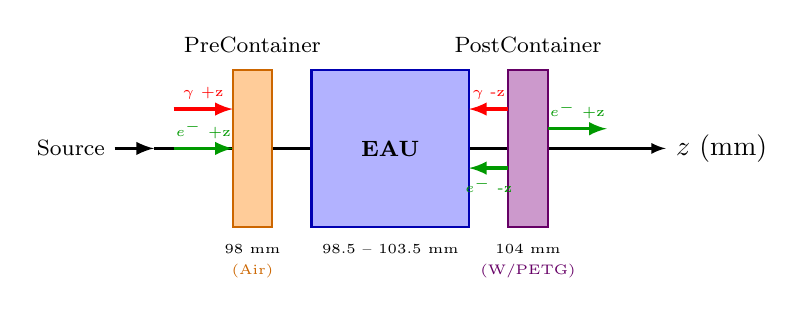
\begin{tikzpicture}[scale=0.5, >=latex]
    % Axe z
    \draw[->, thick] (-1,0) -- (12,0) node[right] {$z$ (mm)};
    
    % PreContainerPlane
    \fill[orange!40] (1,-2) rectangle (2,2);
    \draw[orange!80!black, thick] (1,-2) rectangle (2,2);
    \node[above, font=\footnotesize] at (1.5,2.2) {PreContainer};
    \node[below, font=\tiny] at (1.5,-2.2) {98 mm};
    \node[below, font=\tiny, orange!80!black] at (1.5,-2.7) {(Air)};
    
    % Eau
    \fill[blue!30] (3,-2) rectangle (7,2);
    \draw[blue!70!black, thick] (3,-2) rectangle (7,2);
    \node[font=\footnotesize] at (5,0) {\textbf{EAU}};
    \node[below, font=\tiny] at (5,-2.2) {98.5 -- 103.5 mm};
    
    % PostContainerPlane
    \fill[violet!40] (8,-2) rectangle (9,2);
    \draw[violet!80!black, thick] (8,-2) rectangle (9,2);
    \node[above, font=\footnotesize] at (8.5,2.2) {PostContainer};
    \node[below, font=\tiny] at (8.5,-2.2) {104 mm};
    \node[below, font=\tiny, violet!80!black] at (8.5,-2.7) {(W/PETG)};
    
    % Flèches PreContainer
    \draw[->, red, very thick] (-0.5,1) -- (1,1);
    \node[above, font=\tiny, red] at (0.25,1) {$\gamma$ +z};
    \draw[->, green!60!black, very thick] (-0.5,0) -- (1,0);
    \node[above, font=\tiny, green!60!black] at (0.25,0) {$e^-$ +z};
    
    % Flèches PostContainer (backward)
    \draw[<-, red, very thick] (7,1) -- (8,1);
    \node[above, font=\tiny, red] at (7.5,1) {$\gamma$ -z};
    \draw[<-, green!60!black, very thick] (7,-0.5) -- (8,-0.5);
    \node[below, font=\tiny, green!60!black] at (7.5,-0.5) {$e^-$ -z};
    
    % Flèches PostContainer (forward)
    \draw[->, green!60!black, very thick] (9,0.5) -- (10.5,0.5);
    \node[above, font=\tiny, green!60!black] at (9.75,0.5) {$e^-$ +z};
    
    % Source
    \draw[->, black, very thick] (-2,0) -- (-1,0);
    \node[left, font=\footnotesize] at (-2,0) {Source};
    
\end{tikzpicture}
\end{center}

\vspace{0.5cm}

\begin{table}[h]
\centering
\captionsetup{labelformat=empty}
\caption{\footnotesize Récapitulatif des variables par plan}
\begin{tabular}{lll}
\toprule
\footnotesize \textbf{Plan} &\footnotesize  \textbf{Particule} &\footnotesize  \textbf{Variables} \\
\midrule
\multirow{2}{*}{\footnotesize PreContainerPlane}&\footnotesize $\gamma$ vers eau (+z)&\footnotesize \texttt{nPhotons},\texttt{sumEPhotons\_keV} \\
              &\footnotesize $e^-$ vers eau (+z)&\footnotesize \texttt{nElectrons}, \texttt{sumEElectrons\_keV} \\
\midrule
\multirow{3}{*}{\footnotesize PostContainerPlane}&\footnotesize $\gamma$ depuis eau (-z)&\footnotesize \texttt{nPhotons\_back},\texttt{sumEPhotons\_back\_keV}\\
                &\footnotesize  $e^-$ depuis eau (-z)&\footnotesize \texttt{nElectrons\_back},\texttt{sumEElectrons\_back\_keV} \\
                &\footnotesize   vers eau (+z)&\footnotesize \texttt{nElectrons\_fwd},\texttt{sumEElectrons\_fwd\_keV} \\
\bottomrule
\end{tabular}
\end{table}

%===============================================================================
\normalsize
\noindent \begin{mdframed}[backgroundcolor=orange!20]
\subsection{\color{blue}\textbf{Flux de particules dans les plans Precontainer et Postcontainer avec le filtre ${W/PETG}$ de 5mm}\color{black}}
\end{mdframed}
\footnotesize
%===============================================================================
\medskip

\begin{tcolorbox}[colback=headerblue!10,colframe=headerblue!80!black,title=\textbf{Filtre W/PETG 5mm}]
\noindent Ci aprés les spectres des distributions des photons et électrons dans les plans de comptage PrecontainerPlane et PostContainerPlane\begin{itemize}
    \item photons et électrons dans le \color{blue}\textbf{PreContainerPlane}\color{black}
    \item photons dans le \color{blue}\textbf{PostContainerPlane}\color{black}
    \item électrons "`backward"' retrodiffusés dans le \color{blue}\textbf{PostContainerPlane}\color{black} 
    \item électrons "`forward"' diffusés dans le \color{blue}\textbf{PostContainerPlane}\color{black} 
\end{itemize}
\end{tcolorbox}

\begin{figure}[h!]
    \centering
    \includegraphics[scale=0.4]{Figures/histos_precontainer_FiltreWPETG5mm.png}
		\captionsetup{labelformat=empty}
    \caption{photons et électrons dans le \color{blue}\textbf{PreContainerPlane}\color{black} \; avec le filtre de $\bm{W/PETG}$ de 5mm}
\end{figure}

\begin{figure}[h!]
    \centering
    \includegraphics[scale=0.4]{Figures/histos_postcontainer_electrons_back_FiltreWPETG5mm.png}
		\captionsetup{labelformat=empty}
    \caption{photons dans le \color{blue}\textbf{PostContainerPlane}\color{black} \; avec le filtre de $\bm{W/PETG}$ de 5mm}
\end{figure}

\begin{figure}[h!]
    \centering
    \includegraphics[scale=0.4]{Figures/histos_postcontainer_electrons_fwd_FiltreWPETG5mm.png}
		\captionsetup{labelformat=empty}
    \caption{électrons "`backward"' retrodiffusés dans le \color{blue}\textbf{PostContainerPlane}\color{black} \; avec le filtre de $\bm{W/PETG}$ de 5mm}
\end{figure}

\begin{figure}[h!]
    \centering
    \includegraphics[scale=0.4]{Figures/histos_postcontainer_photons_FiltreWPETG5mm.png}
		\captionsetup{labelformat=empty}
    \caption{électrons "`forward"' diffusés dans le \color{blue}\textbf{PostContainerPlane}\color{black} \; avec le filtre de $\bm{W/PETG}$ de 5mm}
\end{figure}

\clearpage


%===============================================================================
\normalsize
\noindent \begin{mdframed}[backgroundcolor=orange!20]
\subsection{\color{blue}\textbf{Résultats sans le filtre ${W/PETG}$}\color{black}}
\end{mdframed}
\footnotesize
%===============================================================================
\medskip

\begin{tcolorbox}[colback=headerblue!10,colframe=headerblue!80!black,title=\textbf{sans Filtre W/PETG 5mm}]
\noindent On enlève le filtre de $\bm{W/PETG}$
\end{tcolorbox}

\begin{table}[h]
    \centering
		\captionsetup{labelformat=empty}
    \caption{\footnotesize Doses déposées dans les anneaux d'eau -- Simulation avec filtre en \textbf{air} ($10^6$ désintégrations Eu-152)}
\begin{tabular}{c S[table-format=1.4] S[table-format=1.3e2] S[table-format=1.3e2] S[table-format=1.3e2] r}
\toprule
\footnotesize \textbf{Anneau}&\footnotesize {\textbf{Masse}}&\footnotesize {\textbf{$E_{dep}$}}&\footnotesize {\textbf{Dose}}&\footnotesize  {\textbf{Dose/evt}}&\footnotesize \textbf{Événements}\\
 &\footnotesize  {(g)} &\footnotesize {(MeV)}&\footnotesize  {(nGy)} &\footnotesize{(nGy)} & \\
 \midrule
 \footnotesize 0 (r=0--5 mm)&\footnotesize 0.3927&\footnotesize 4.407e2&\footnotesize 1.798e2&\footnotesize 6.762e-2&\footnotesize 2\,659 \\
 \footnotesize 1 (r=5--10 mm)&\footnotesize 1.1781&\footnotesize 1.307e3&\footnotesize 1.778e2&\footnotesize 2.274e-2&\footnotesize 7\,818 \\
 \footnotesize 2 (r=10--15 mm)&\footnotesize 1.9635&\footnotesize2.184e3&\footnotesize 1.782e2&\footnotesize 1.356e-2&\footnotesize 13\,144 \\
 \footnotesize 3 (r=15--20 mm)&\footnotesize 2.7489&\footnotesize 2.970e3&\footnotesize 1.731e2&\footnotesize 9.703e-3&\footnotesize 17\,843 \\
\footnotesize 4 (r=20--25 mm)&\footnotesize 3.5343&\footnotesize 3.970e3&\footnotesize 1.800e2&\footnotesize 7.773e-3&\footnotesize 23\,152 \\
\midrule
\footnotesize \textbf{TOTAL}&\footnotesize \textbf{9.8175}&\footnotesize \textbf{1.087e4}&\footnotesize \textbf{1.774e2}&\footnotesize \textbf{1.774e-4} &\footnotesize\textbf{1\,000\,000} \\
\bottomrule
\end{tabular}
\end{table}

% Version simplifiée sans notation scientifique pour certaines colonnes
\begin{table}[h]
\centering
\captionsetup{labelformat=empty}
\caption{\footnotesize Doses déposées dans les anneaux d'eau -- Version simplifiée}
\begin{tabular}{ccccc}
\toprule
\footnotesize\textbf{Anneau}&\footnotesize \textbf{Rayon (mm)}&\footnotesize \textbf{Masse (g)}&\footnotesize \textbf{Dose (nGy)}&\footnotesize \textbf{Dose/désint. (nGy)} \\
\midrule
\footnotesize0&\footnotesize 0 -- 5&\footnotesize 0.393&\footnotesize 179.8&\footnotesize $6.76 \times 10^{-2}$ \\
\footnotesize1&\footnotesize 5 -- 10&\footnotesize 1.178&\footnotesize 177.8&\footnotesize $2.27 \times 10^{-2}$ \\
\footnotesize2&\footnotesize 10 -- 15&\footnotesize 1.964&\footnotesize 178.2&\footnotesize $1.36 \times 10^{-2}$ \\
\footnotesize3&\footnotesize 15 -- 20&\footnotesize 2.749&\footnotesize 173.1&\footnotesize $9.70 \times 10^{-3}$ \\
\footnotesize4&\footnotesize 20 -- 25&\footnotesize 3.534&\footnotesize 180.0&\footnotesize $7.77 \times 10^{-3}$ \\
\midrule
\multicolumn{2}{c}{\footnotesize\textbf{TOTAL}}&\footnotesize \textbf{9.817}&\footnotesize \textbf{177.4}&\footnotesize $\mathbf{1.77 \times 10^{-4}}$ \\
\bottomrule
\end{tabular}
\end{table}

% Tableau comparatif avec/sans filtre W_PETG
\begin{table}[h]
\centering
\captionsetup{labelformat=empty}
\caption{\footnotesize Comparaison des doses : filtre W/PETG vs filtre Air}
\begin{tabular}{ccccc}
\toprule
\footnotesize\textbf{Anneau}&\footnotesize \textbf{Rayon (mm)}&\footnotesize \textbf{Dose W/PETG (nGy)}&\footnotesize \textbf{Dose Air (nGy)} &\footnotesize \textbf{Augmentation} \\
\midrule
\footnotesize 0&\footnotesize 0 -- 5&\footnotesize 148.4&\footnotesize 179.8&\footnotesize +21.2\% \\
\footnotesize 1&\footnotesize 5 -- 10&\footnotesize 159.7&\footnotesize 177.8&\footnotesize +11.3\% \\
\footnotesize 2&\footnotesize 10 -- 15&\footnotesize 155.3&\footnotesize 178.2&\footnotesize +14.7\% \\
\footnotesize 3&\footnotesize 15 -- 20&\footnotesize 149.2&\footnotesize 173.1&\footnotesize +16.0\% \\
\footnotesize 4&\footnotesize 20 -- 25&\footnotesize 153.7&\footnotesize 180.0&\footnotesize +17.1\% \\
\midrule
\multicolumn{2}{c}{\footnotesize\textbf{TOTAL}}&\footnotesize \textbf{153.3}&\footnotesize\textbf{177.4}&\footnotesize \textbf{+15.7\%} \\
\bottomrule
\end{tabular}
\end{table}

\begin{tcolorbox}[colback=headerblue!10,colframe=headerblue!80!black,title=\textbf{Filtre W/PETG 5mm}]
\noindent Ci aprés les spectres des distributions des photons et électrons dans les plans de comptage PrecontainerPlane et PostContainerPlane
\begin{itemize}
    \item photons et électrons dans le \color{blue}\textbf{PreContainerPlane}\color{black}
    \item photons dans le \color{blue}\textbf{PostContainerPlane}\color{black}
    \item électrons "`backward"' retrodiffusés dans le \color{blue}\textbf{PostContainerPlane}\color{black} 
    \item électrons "`forward"' diffusés dans le \color{blue}\textbf{PostContainerPlane}\color{black} 
\end{itemize}
\end{tcolorbox}

\begin{figure}[h!]
    \centering
    \includegraphics[scale=0.4]{Figures/histos_precontainer_FiltreWPETG5mm.png}
		\captionsetup{labelformat=empty}
    \caption{photons et électrons dans le \color{blue}\textbf{PreContainerPlane}\color{black} \; sans le filtre de $\bm{W/PETG}$ de 5mm}
\end{figure}

\begin{figure}[h!]
    \centering
    \includegraphics[scale=0.4]{Figures/histos_postcontainer_electrons_back_FiltreWPETG5mm.png}
		\captionsetup{labelformat=empty}
    \caption{photons dans le \color{blue}\textbf{PostContainerPlane}\color{black} \; sans le filtre de $\bm{W/PETG}$ de 5mm}
\end{figure}

\begin{figure}[h!]
    \centering
    \includegraphics[scale=0.4]{Figures/histos_postcontainer_electrons_fwd_FiltreWPETG5mm.png}
		\captionsetup{labelformat=empty}
    \caption{électrons "`backward"' retrodiffusés dans le \color{blue}\textbf{PostContainerPlane}\color{black} \; sans le filtre de $\bm{W/PETG}$ de 5mm}
\end{figure}

\begin{figure}[H]
    \centering
    \includegraphics[scale=0.4]{Figures/histos_postcontainer_photons_FiltreWPETG5mm.png}
		\captionsetup{labelformat=empty}
    \caption{électrons "`forward"' diffusés dans le \color{blue}\textbf{PostContainerPlane}\color{black} \; sans le filtre de $\bm{W/PETG}$ de 5mm}
\end{figure}

\clearpage

%==============================================================================
\normalsize
\noindent \begin{mdframed}[backgroundcolor=orange!20]
\section{\Large \color{blue} \textbf{Insertion d'une plaque de PMMA et d'une feuille de W pour améliorer le build-up dans l'eau}\color{black}}
\end{mdframed}
\footnotesize
%==============================================================================

\begin{tcolorbox}[colback=blue!5,colframe=blue,title=\textbf{Changement de géométrie}]
\noindent Le container d'eau est précédé d'une \color{blue}\textbf{plaque de PMMA de 5 mm d'epaisseur}\color{black}, pour améliorer la conversion des photons incidents et la \color{blue}\textbf{production d'électrons secondaires}\color{black}  dans l'eau du container. L'objectif de ce plan est d'améliorer le build-up electronique\newline
\noindent Le fond du container d'eau est tapissé d'une \color{blue}\textbf{feuille de tungstène}\color{black} pour améliorer la \color{blue}\textbf{rétrodiffusion des électrons}\color{black} produit par les photons incidents dans la feuille de tungsténe. L'objectif de ce plan est d'améliorer le build-up electronique\newline
\end{tcolorbox}

\begin{table}[h]
\centering
\caption{\footnotesize Positions axiales (z) des éléments de la géométrie du container}
\captionsetup{labelformat=empty}
\begin{tabular}{llcccc}
\toprule
\footnotesize \textbf{Élément}&\footnotesize \textbf{Matériau}&\footnotesize \textbf{$z_{min}$}&\footnotesize \textbf{$z_{max}$}& \footnotesize \textbf{Épaisseur} &\footnotesize  \textbf{Rayon} \\
  & &\footnotesize (mm)&\footnotesize (mm) &\footnotesize &\footnotesize  (mm)\\
\midrule
\rowcolor{pmma!50}
\footnotesize PMMA&\footnotesize PMMA&\footnotesize 92.50&\footnotesize 97.50&\footnotesize 5 mm &\footnotesize  25 \\
\rowcolor{preplane!30}
\footnotesize PreContainerPlane&\footnotesize Air&\footnotesize 97.50&\footnotesize 98.50&\footnotesize 1 mm &\footnotesize  25 \\
\rowcolor{water!50}
\footnotesize Eau (5 anneaux)&\footnotesize H$_2$O&\footnotesize 98.50&\footnotesize 103.50&\footnotesize  5 mm&\footnotesize  25 \\
\rowcolor{postplane!50}
\footnotesize PostContainerPlane&\footnotesize Air&\footnotesize 102.50&\footnotesize 103.50&\footnotesize 1 mm &\footnotesize 25 \\
\rowcolor{tungsten!50}
\footnotesize Feuille W&\footnotesize Tungstène&\footnotesize 103.50&\footnotesize 103.52&\footnotesize 20 $\mu$m&\footnotesize  25 \\
\rowcolor{wpetg!30}
\footnotesize Fond container&\footnotesize  W/PETG&\footnotesize 103.50&\footnotesize 105.50 &\footnotesize 2 mm &\footnotesize  30 \\
\rowcolor{wpetg!30}
\footnotesize Parois container&\footnotesize W/PETG&\footnotesize 92.50&\footnotesize  105.50&\footnotesize 5 mm (radial)&\footnotesize  25--30 \\
\bottomrule
\end{tabular}
\end{table}

%===============================================================================
\normalsize
\noindent \begin{mdframed}[backgroundcolor=orange!20]
\subsection{\color{blue}\textbf{Vue en coupe de la géométrie}\color{black}}
\end{mdframed}
\footnotesize
%===============================================================================
\medskip

\noindent La figure suivante présente une vue en coupe axiale (plan XZ) de la géométrie du container et des plans de comptage associés.

\begin{figure}[h!]
\centering
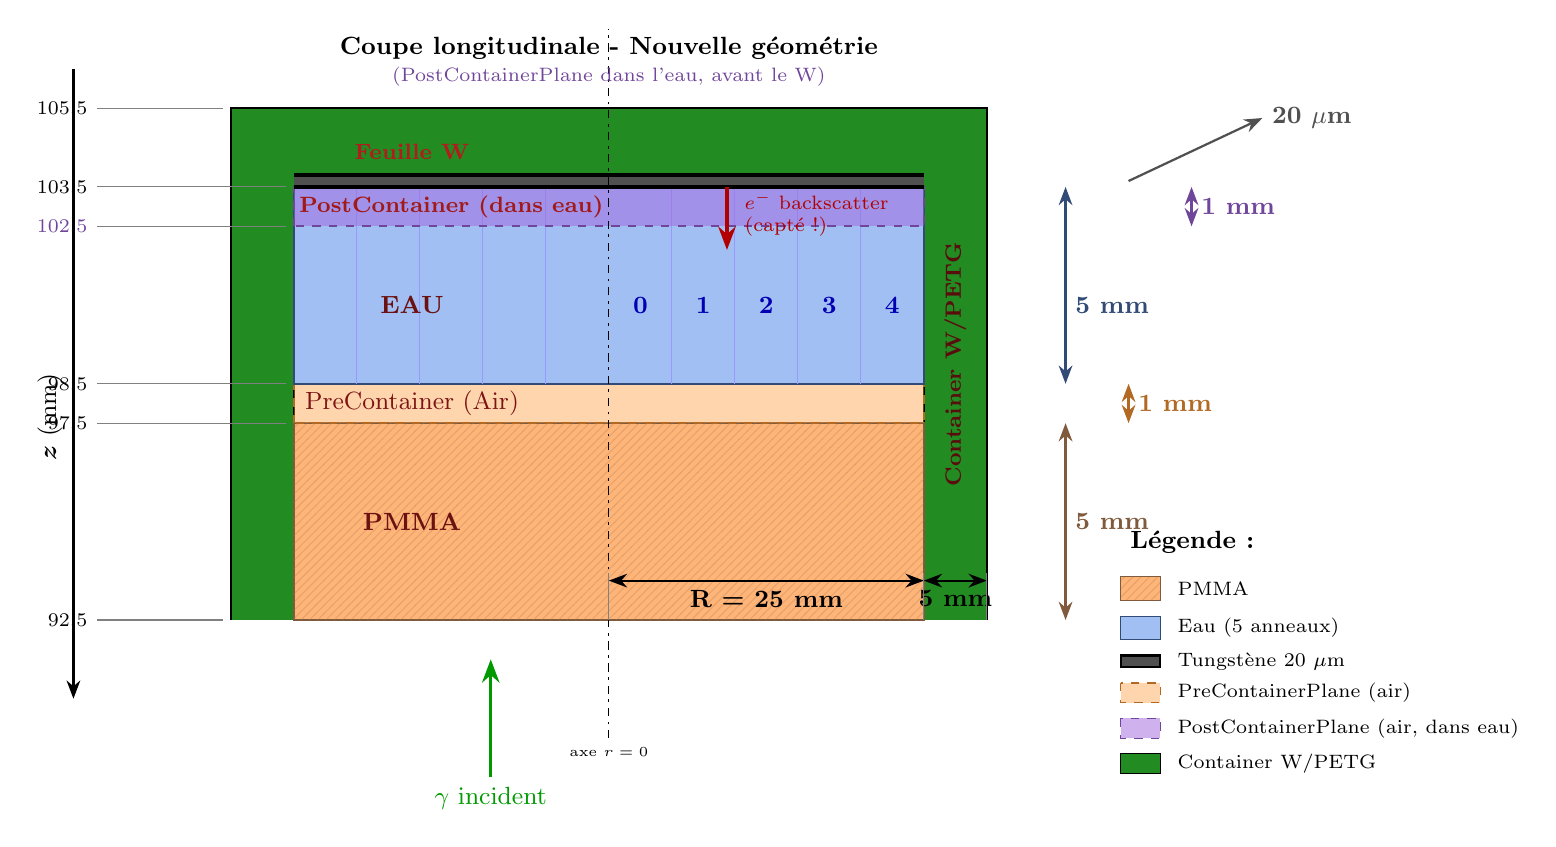
\begin{tikzpicture}[>=Stealth, font=\small]

    % ═══════════════════════════════════════════════════════════════════════
    % ÉCHELLE : 1 unité TikZ = 1 mm
    % Facteur d'échelle horizontal (r) : 0.16
    % Facteur d'échelle vertical (z) : 0.5
    % ═══════════════════════════════════════════════════════════════════════
    
    \def\scaleR{0.16}
    \def\scaleZ{0.5}
    
    % ═══════════════════════════════════════════════════════════════════════
    % NOUVELLE GÉOMÉTRIE (PostContainerPlane DANS l'eau, AVANT le W)
    % ═══════════════════════════════════════════════════════════════════════
    
    % Positions z (en mm)
    \def\zPMMAbot{92.5}
    \def\zPMMAtop{97.5}
    \def\zPreBot{97.5}
    \def\zPreTop{98.5}
    \def\zWaterBot{98.5}
    \def\zWaterTop{103.5}
    % MODIFIÉ : PostContainerPlane maintenant DANS l'eau (102.5 - 103.5 mm)
    \def\zPostBot{102.5}
    \def\zPostTop{103.5}
    % Feuille de tungstène juste après le haut de l'eau/PostContainer
    \def\zTungstenBot{103.5}
    \def\zTungstenTop{103.52}
    \def\zContainerBot{103.5}
    \def\zContainerTop{105.5}
    
    % Rayons (en mm)
    \def\Rinner{25}
    \def\Router{30}
    
    % Décalage pour centrer
    \def\zoff{-98}
    
    % ═══════════════════════════════════════════════════════════════════════
    % DESSIN DES ÉLÉMENTS (de bas en haut)
    % ═══════════════════════════════════════════════════════════════════════
    
    % --- Parois du container (W/PETG) ---
    \fill[wpetg] ({-\Router*\scaleR}, {(\zPMMAbot+\zoff)*\scaleZ}) rectangle ({-\Rinner*\scaleR}, {(\zContainerTop+\zoff)*\scaleZ});
    \fill[wpetg] ({\Rinner*\scaleR}, {(\zPMMAbot+\zoff)*\scaleZ}) rectangle ({\Router*\scaleR}, {(\zContainerTop+\zoff)*\scaleZ});
    % Fond du container
    \fill[wpetg] ({-\Router*\scaleR}, {(\zContainerBot+\zoff)*\scaleZ}) rectangle ({\Router*\scaleR}, {(\zContainerTop+\zoff)*\scaleZ});
    
    % Contours container
    \draw[black, thick] ({-\Router*\scaleR}, {(\zPMMAbot+\zoff)*\scaleZ}) -- ({-\Router*\scaleR}, {(\zContainerTop+\zoff)*\scaleZ}) -- ({\Router*\scaleR}, {(\zContainerTop+\zoff)*\scaleZ}) -- ({\Router*\scaleR}, {(\zPMMAbot+\zoff)*\scaleZ});
    \draw[black, thick] ({-\Rinner*\scaleR}, {(\zPMMAbot+\zoff)*\scaleZ}) -- ({-\Rinner*\scaleR}, {(\zContainerBot+\zoff)*\scaleZ}) -- ({\Rinner*\scaleR}, {(\zContainerBot+\zoff)*\scaleZ}) -- ({\Rinner*\scaleR}, {(\zPMMAbot+\zoff)*\scaleZ});
    
    % --- PMMA (5 mm) ---
    \fill[pmma] ({-\Rinner*\scaleR}, {(\zPMMAbot+\zoff)*\scaleZ}) rectangle ({\Rinner*\scaleR}, {(\zPMMAtop+\zoff)*\scaleZ});
    \draw[pmma!50!black, thick] ({-\Rinner*\scaleR}, {(\zPMMAbot+\zoff)*\scaleZ}) rectangle ({\Rinner*\scaleR}, {(\zPMMAtop+\zoff)*\scaleZ});
    % Hachures PMMA
    \fill[pattern=north east lines, pattern color=pmma!70!black, opacity=0.3] ({-\Rinner*\scaleR}, {(\zPMMAbot+\zoff)*\scaleZ}) rectangle ({\Rinner*\scaleR}, {(\zPMMAtop+\zoff)*\scaleZ});
    
    % --- PreContainerPlane (1 mm, air) ---
    \fill[preplane, opacity=0.4] ({-\Rinner*\scaleR}, {(\zPreBot+\zoff)*\scaleZ}) rectangle ({\Rinner*\scaleR}, {(\zPreTop+\zoff)*\scaleZ});
    \draw[preplane!70!black, thick, dashed] ({-\Rinner*\scaleR}, {(\zPreBot+\zoff)*\scaleZ}) rectangle ({\Rinner*\scaleR}, {(\zPreTop+\zoff)*\scaleZ});
    
    % --- Eau (5 mm, 5 anneaux) ---
    \fill[water, opacity=0.6] ({-\Rinner*\scaleR}, {(\zWaterBot+\zoff)*\scaleZ}) rectangle ({\Rinner*\scaleR}, {(\zWaterTop+\zoff)*\scaleZ});
    \draw[water!50!black, thick] ({-\Rinner*\scaleR}, {(\zWaterBot+\zoff)*\scaleZ}) rectangle ({\Rinner*\scaleR}, {(\zWaterTop+\zoff)*\scaleZ});
    % Limites des anneaux
    \foreach \r in {5, 10, 15, 20} {
        \draw[blue!40, thin] ({-\r*\scaleR}, {(\zWaterBot+\zoff)*\scaleZ}) -- ({-\r*\scaleR}, {(\zWaterTop+\zoff)*\scaleZ});
        \draw[blue!40, thin] ({\r*\scaleR}, {(\zWaterBot+\zoff)*\scaleZ}) -- ({\r*\scaleR}, {(\zWaterTop+\zoff)*\scaleZ});
    }
    % Labels anneaux
    \node[font=\small, blue!70!black] at ({2.5*\scaleR}, {(100.5+\zoff)*\scaleZ}) {\textbf{0}};
    \node[font=\small, blue!70!black] at ({7.5*\scaleR}, {(100.5+\zoff)*\scaleZ}) {\textbf{1}};
    \node[font=\small, blue!70!black] at ({12.5*\scaleR}, {(100.5+\zoff)*\scaleZ}) {\textbf{2}};
    \node[font=\small, blue!70!black] at ({17.5*\scaleR}, {(100.5+\zoff)*\scaleZ}) {\textbf{3}};
    \node[font=\small, blue!70!black] at ({22.5*\scaleR}, {(100.5+\zoff)*\scaleZ}) {\textbf{4}};
    
    % --- PostContainerPlane (1 mm, AIR) - MAINTENANT DANS L'EAU ---
    \fill[postplane, opacity=0.5] ({-\Rinner*\scaleR}, {(\zPostBot+\zoff)*\scaleZ}) rectangle ({\Rinner*\scaleR}, {(\zPostTop+\zoff)*\scaleZ});
    \draw[postplane!70!black, thick, dashed] ({-\Rinner*\scaleR}, {(\zPostBot+\zoff)*\scaleZ}) rectangle ({\Rinner*\scaleR}, {(\zPostTop+\zoff)*\scaleZ});
    
    % --- Feuille de Tungstène (20 µm) - épaisseur exagérée pour visibilité ---
    \def\Wthick{0.15}  % Épaisseur visuelle exagérée
    \fill[tungsten] ({-\Rinner*\scaleR}, {(\zTungstenBot+\zoff)*\scaleZ}) rectangle ({\Rinner*\scaleR}, {(\zTungstenBot+\zoff)*\scaleZ + \Wthick});
    \draw[black, very thick] ({-\Rinner*\scaleR}, {(\zTungstenBot+\zoff)*\scaleZ}) -- ({\Rinner*\scaleR}, {(\zTungstenBot+\zoff)*\scaleZ});
    \draw[black, very thick] ({-\Rinner*\scaleR}, {(\zTungstenBot+\zoff)*\scaleZ + \Wthick}) -- ({\Rinner*\scaleR}, {(\zTungstenBot+\zoff)*\scaleZ + \Wthick});
    
    % ═══════════════════════════════════════════════════════════════════════
    % AXE DE SYMÉTRIE
    % ═══════════════════════════════════════════════════════════════════════
    
    \draw[black, dash pattern=on 3pt off 2pt on 1pt off 2pt, thin] (0, {(\zPMMAbot+\zoff-3)*\scaleZ}) -- (0, {(\zContainerTop+\zoff+2)*\scaleZ});
    \node[below, font=\tiny] at (0, {(\zPMMAbot+\zoff-3)*\scaleZ}) {axe $r=0$};
    
    % ═══════════════════════════════════════════════════════════════════════
    % COTES VERTICALES (positions z) - À GAUCHE
    % ═══════════════════════════════════════════════════════════════════════
    
    \def\cotex{-6.5}
    
    % Ligne de référence
    \draw[gray, thin] ({\cotex}, {(\zPMMAbot+\zoff)*\scaleZ}) -- ({-\Router*\scaleR-0.1}, {(\zPMMAbot+\zoff)*\scaleZ});
    \draw[gray, thin] ({\cotex}, {(\zPMMAtop+\zoff)*\scaleZ}) -- ({-\Rinner*\scaleR-0.1}, {(\zPMMAtop+\zoff)*\scaleZ});
    \draw[gray, thin] ({\cotex}, {(\zPreTop+\zoff)*\scaleZ}) -- ({-\Rinner*\scaleR-0.1}, {(\zPreTop+\zoff)*\scaleZ});
    \draw[gray, thin] ({\cotex}, {(\zPostBot+\zoff)*\scaleZ}) -- ({-\Rinner*\scaleR-0.1}, {(\zPostBot+\zoff)*\scaleZ});
    \draw[gray, thin] ({\cotex}, {(\zWaterTop+\zoff)*\scaleZ}) -- ({-\Rinner*\scaleR-0.1}, {(\zWaterTop+\zoff)*\scaleZ});
    \draw[gray, thin] ({\cotex}, {(\zContainerTop+\zoff)*\scaleZ}) -- ({-\Router*\scaleR-0.1}, {(\zContainerTop+\zoff)*\scaleZ});
    
    % Valeurs z
    \node[left, font=\scriptsize] at ({\cotex}, {(\zPMMAbot+\zoff)*\scaleZ}) {92.5};
    \node[left, font=\scriptsize] at ({\cotex}, {(\zPMMAtop+\zoff)*\scaleZ}) {97.5};
    \node[left, font=\scriptsize] at ({\cotex}, {(\zPreTop+\zoff)*\scaleZ}) {98.5};
    \node[left, font=\scriptsize, postplane!70!black] at ({\cotex}, {(\zPostBot+\zoff)*\scaleZ}) {102.5};
    \node[left, font=\scriptsize] at ({\cotex}, {(\zWaterTop+\zoff)*\scaleZ}) {103.5};
    \node[left, font=\scriptsize] at ({\cotex}, {(\zContainerTop+\zoff)*\scaleZ}) {105.5};
    
    % Label axe z
    \draw[<-, thick] ({\cotex-0.3}, {(\zPMMAbot+\zoff-2)*\scaleZ}) -- ({\cotex-0.3}, {(\zContainerTop+\zoff+1)*\scaleZ});
    \node[left, font=\small, rotate=90] at ({\cotex-0.6}, {(99+\zoff)*\scaleZ}) {$\bm{z}$ (mm)};
    
    % ═══════════════════════════════════════════════════════════════════════
    % COTES DES ÉPAISSEURS - À DROITE
    % ═══════════════════════════════════════════════════════════════════════
    
    \def\cotexR{5.8}
    
    % PMMA : 5 mm
    \draw[<->, thick, pmma!50!black] ({\cotexR}, {(\zPMMAbot+\zoff)*\scaleZ}) -- ({\cotexR}, {(\zPMMAtop+\zoff)*\scaleZ});
    \node[right, font=\small, pmma!50!black] at ({\cotexR}, {(95+\zoff)*\scaleZ}) {\textbf{5 mm}};
    
    % PreContainerPlane : 1 mm
    \draw[<->, thick, preplane!70!black] ({\cotexR+0.8}, {(\zPreBot+\zoff)*\scaleZ}) -- ({\cotexR+0.8}, {(\zPreTop+\zoff)*\scaleZ});
    \node[right, font=\small, preplane!70!black] at ({\cotexR+0.8}, {(98+\zoff)*\scaleZ}) {\textbf{1 mm}};
    
    % Eau : 5 mm
    \draw[<->, thick, water!50!black] ({\cotexR}, {(\zWaterBot+\zoff)*\scaleZ}) -- ({\cotexR}, {(\zWaterTop+\zoff)*\scaleZ});
    \node[right, font=\small, water!50!black] at ({\cotexR}, {(100.5+\zoff)*\scaleZ}) {\textbf{5 mm}};
    
    % PostContainerPlane : 1 mm (DANS L'EAU)
    \draw[<->, thick, postplane!70!black] ({\cotexR+1.6}, {(\zPostBot+\zoff)*\scaleZ}) -- ({\cotexR+1.6}, {(\zPostTop+\zoff)*\scaleZ});
    \node[right, font=\small, postplane!70!black] at ({\cotexR+1.6}, {(103+\zoff)*\scaleZ}) {\textbf{1 mm}};
    
    % Tungstène : 20 µm (avec flèche vers zoom)
    \draw[->, thick, tungsten] ({\cotexR+0.8}, {(\zTungstenBot+\zoff)*\scaleZ + \Wthick/2}) -- ({\cotexR+2.5}, {(\zTungstenBot+\zoff)*\scaleZ + \Wthick/2 + 0.8});
    \node[right, font=\small, tungsten] at ({\cotexR+2.5}, {(\zTungstenBot+\zoff)*\scaleZ + \Wthick/2 + 0.8}) {\textbf{20 $\mu$m}};
    
    % ═══════════════════════════════════════════════════════════════════════
    % COTES HORIZONTALES (rayons) - EN BAS
    % ═══════════════════════════════════════════════════════════════════════
    
    \def\cotey{-4.5}
    
    % R = 25 mm
    \draw[<->, thick] (0, {\cotey*\scaleZ}) -- ({\Rinner*\scaleR}, {\cotey*\scaleZ});
    \node[below, font=\small] at ({12.5*\scaleR}, {\cotey*\scaleZ}) {\textbf{R = 25 mm}};
    
    % Paroi = 5 mm
    \draw[<->, thick] ({\Rinner*\scaleR}, {\cotey*\scaleZ}) -- ({\Router*\scaleR}, {\cotey*\scaleZ});
    \node[below, font=\small] at ({27.5*\scaleR}, {\cotey*\scaleZ}) {\textbf{5 mm}};
    
    % Lignes de rappel
    \draw[gray, thin] (0, {(\zPMMAbot+\zoff)*\scaleZ}) -- (0, {\cotey*\scaleZ + 0.1});
    \draw[gray, thin] ({\Rinner*\scaleR}, {(\zPMMAbot+\zoff)*\scaleZ}) -- ({\Rinner*\scaleR}, {\cotey*\scaleZ + 0.1});
    \draw[gray, thin] ({\Router*\scaleR}, {(\zPMMAbot+\zoff)*\scaleZ}) -- ({\Router*\scaleR}, {\cotey*\scaleZ + 0.1});
    
    % ═══════════════════════════════════════════════════════════════════════
    % LABELS DES MATÉRIAUX
    % ═══════════════════════════════════════════════════════════════════════
    
    \def\labelx{-2.5}
    
    % PMMA
    \node[font=\small\bfseries, Carnelian!60!black] at ({\labelx}, {(95+\zoff)*\scaleZ}) {\textbf{PMMA}};
    
    % PreContainerPlane
    \node[font=\small, Carnelian!70!black, align=center] at ({\labelx}, {(98+\zoff)*\scaleZ}) {PreContainer (Air)};
    
    % Eau
    \node[font=\small\bfseries, Carnelian!60!black] at ({\labelx}, {(100.5+\zoff)*\scaleZ}) {\textbf{EAU}};
    
    % PostContainerPlane (DANS L'EAU)
    \node[font=\footnotesize\bfseries, Carnelian!90!black, align=center] at ({\labelx+0.5}, {(103+\zoff)*\scaleZ}) {PostContainer (dans eau)};
    
    % Tungstène
    \node[font=\footnotesize\bfseries, Carnelian] at ({\labelx}, {(103.5+\zoff)*\scaleZ + \Wthick + 0.3}) {\textbf{Feuille W}};
    
    % Container
    \node[font=\footnotesize, Carnelian!50!black, rotate=90] at ({(\Rinner+2.5)*\scaleR}, {(99+\zoff)*\scaleZ}) {\textbf{Container W/PETG}};
    
    % ═══════════════════════════════════════════════════════════════════════
    % FLÈCHES POUR LE BACKSCATTER
    % ═══════════════════════════════════════════════════════════════════════
    
    % Flèche photon incident
    \draw[->, very thick, green!60!black] (-1.5, {(\zPMMAbot+\zoff-4)*\scaleZ}) -- (-1.5, {(\zPMMAbot+\zoff-1)*\scaleZ});
    \node[below, font=\small, green!60!black] at (-1.5, {(\zPMMAbot+\zoff-4)*\scaleZ}) {$\gamma$ incident};
    
    % Flèche électron backscatter du W (vers -z)
    \draw[->, very thick, red!70!black] (1.5, {(\zTungstenBot+\zoff)*\scaleZ}) -- (1.5, {(\zPostBot+\zoff)*\scaleZ - 0.3});
    \node[right, font=\scriptsize, red!70!black, align=left] at (1.6, {(102.8+\zoff)*\scaleZ}) {$e^-$ backscatter\\(capté !)};
    
    % ═══════════════════════════════════════════════════════════════════════
    % TITRE
    % ═══════════════════════════════════════════════════════════════════════
    
    \node[above, font=\small\bfseries] at (0, {(\zContainerTop+\zoff+1)*\scaleZ}) {Coupe longitudinale - Nouvelle géométrie};
    \node[above, font=\scriptsize, postplane!70!black] at (0, {(\zContainerTop+\zoff+0.3)*\scaleZ}) {(PostContainerPlane dans l'eau, avant le W)};
    
    % ═══════════════════════════════════════════════════════════════════════
    % LÉGENDE
    % ═══════════════════════════════════════════════════════════════════════
    
    \def\legx{6.5}
    \def\legy{-1.5}
    
    \node[anchor=north west, font=\small\bfseries] at ({\legx}, {\legy}) {Légende :};
    
    % Espacement vertical entre les éléments de la légende
    \def\legspacing{0.45}
    \def\legstart{0.7}
    
    % PMMA
    \def\ypmma{\legy-\legstart}
    \fill[pmma] ({\legx}, {\ypmma}) rectangle ({\legx+0.5}, {\ypmma-0.3});
    \fill[pattern=north east lines, pattern color=pmma!70!black, opacity=0.3] ({\legx}, {\ypmma}) rectangle ({\legx+0.5}, {\ypmma-0.3});
    \draw[pmma!50!black] ({\legx}, {\ypmma}) rectangle ({\legx+0.5}, {\ypmma-0.3});
    \node[right, font=\scriptsize] at ({\legx+0.6}, {\ypmma-0.15}) {PMMA};
    
    % Eau
    \def\yeau{\legy-\legstart-0.5}
    \fill[water, opacity=0.6] ({\legx}, {\yeau}) rectangle ({\legx+0.5}, {\yeau-0.3});
    \draw[water!50!black] ({\legx}, {\yeau}) rectangle ({\legx+0.5}, {\yeau-0.3});
    \node[right, font=\scriptsize] at ({\legx+0.6}, {\yeau-0.15}) {Eau (5 anneaux)};
    
    % Tungstène
    \def\ytung{\legy-\legstart-1.0}
    \fill[tungsten] ({\legx}, {\ytung}) rectangle ({\legx+0.5}, {\ytung-0.15});
    \draw[black, thick] ({\legx}, {\ytung}) rectangle ({\legx+0.5}, {\ytung-0.15});
    \node[right, font=\scriptsize] at ({\legx+0.6}, {\ytung-0.075}) {Tungstène 20 $\mu$m};
    
    % PreContainerPlane
    \def\ypre{\legy-\legstart-1.35}
    \fill[preplane, opacity=0.4] ({\legx}, {\ypre}) rectangle ({\legx+0.5}, {\ypre-0.25});
    \draw[preplane!70!black, dashed] ({\legx}, {\ypre}) rectangle ({\legx+0.5}, {\ypre-0.25});
    \node[right, font=\scriptsize] at ({\legx+0.6}, {\ypre-0.125}) {PreContainerPlane (air)};
    
    % PostContainerPlane - MODIFIÉ
    \def\ypost{\legy-\legstart-1.8}
    \fill[postplane, opacity=0.5] ({\legx}, {\ypost}) rectangle ({\legx+0.5}, {\ypost-0.25});
    \draw[postplane!70!black, dashed] ({\legx}, {\ypost}) rectangle ({\legx+0.5}, {\ypost-0.25});
    \node[right, font=\scriptsize] at ({\legx+0.6}, {\ypost-0.125}) {PostContainerPlane (air, dans eau)};
    
    % Container
    \def\ycont{\legy-\legstart-2.25}
    \fill[wpetg] ({\legx}, {\ycont}) rectangle ({\legx+0.5}, {\ycont-0.25});
    \draw[black] ({\legx}, {\ycont}) rectangle ({\legx+0.5}, {\ycont-0.25});
    \node[right, font=\scriptsize] at ({\legx+0.6}, {\ycont-0.125}) {Container W/PETG};

\end{tikzpicture}
\captionsetup{labelformat=empty}
\caption{\footnotesize Vue en coupe axiale (plan XZ) du container et des plans de comptage. Les plans de comptage sont représentés avec leur couleur respective : PreContainer (orange) et PostContainer (violet). L'eau est divisée en 5 anneaux concentriques de 5~mm de largeur.}
\end{figure}

%===============================================================================
\normalsize
\noindent \begin{mdframed}[backgroundcolor=orange!20]
\subsection{\color{blue}\textbf{Résultats dans le cas d'une configuration de base}\color{black}}
\end{mdframed}
\footnotesize
%===============================================================================
\medskip

\begin{tcolorbox}[colback=blue!5,colframe=blue,title=\textbf{Géométrie de base}]
\noindent On modifie les matériaux de différents volumes pour avoir une référence. \color{blue}\textbf{On prend comme matériau l'air pour:}\color{black}
\begin{itemize}
\item Les bloc de PMMA,
\item Les anneaux d'eau,
\item la feuille de tungstene 
\item les parois du container
\end{itemize}
\end{tcolorbox}

%===============================================================================
\normalsize
\noindent \begin{mdframed}[backgroundcolor=orange!20]
\subsection{\color{blue}\textbf{Définition des observables}\color{black}}
\end{mdframed}
\footnotesize
%===============================================================================
\medskip

\noindent Les particules sont comptées selon leur \color{blue}\textbf{direction de propagation}\color{black} :

\begin{table}[h]
\centering
\captionsetup{labelformat=empty}
\caption{\footnotesize Définition des observables aux plans de comptage}
\begin{tabular}{lll}
\toprule
\footnotesize \textbf{Plan} &\footnotesize \textbf{Direction} &\footnotesize \textbf{Signification physique} \\
\midrule
\footnotesize PreContainer &\footnotesize $\bm{p_z} > 0$ (+z) &\footnotesize Particules \textbf{entrant} dans la région eau \\
\footnotesize PostContainer &\footnotesize  $\bm{p_z} > 0$ (+z) &\footnotesize Particules \textbf{transmises} (sortant de l'eau) \\
\footnotesize PostContainer &\footnotesize $\bm{p_z} < 0$ (-z) &\footnotesize Particules \textbf{rétrodiffusées} (backscatter) \\
\bottomrule
\end{tabular}
\end{table}

%===============================================================================
\normalsize
\noindent \begin{mdframed}[backgroundcolor=orange!20]
\subsection{\color{blue}\textbf{Résultats pour les Photons}\color{black}}
\end{mdframed}
\footnotesize
%===============================================================================
\medskip

\begin{figure}[h!]
\centering
\includegraphics[scale=0.5]{Figures/histos_precontainer_basic.png}
\captionsetup{labelformat=empty}
\caption{4 histogrammes représentant les particules \textbf{entrant dans la région eau} (direction $\bm{+z}$) : \textbf{Haut gauche} : Nombre de photons par désintégration ($\bm{N_\gamma}$). \textbf{Haut droite} : Somme des énergies des photons ($\bm{\Sigma} \bm{E_\gamma}$ en keV). \textbf{Bas gauche} : Nombre d'électrons par désintégration ($\bm{N_{e^-}}$). \textbf{Bas droite} : Somme des énergies des électrons ($\bm{\Sigma} \bm{E_{e^-}}$ en keV). Le plan Precontainer mesure le flux de particules \textbf{incident} sur la région où se trouve normalement l'eau. C'est la référence pour calculer l'atténuation.}
\end{figure}

\begin{table}[h]
\centering
\captionsetup{labelformat=empty}
\caption{\footnotesize Comparaison des distributions de photons entre \textbf{PreContainer} et \textbf{PostContainer}}
\begin{tabular}{lccc}
\toprule
\footnotesize \textbf{Observable}&\footnotesize \textbf{PreContainer}&\footnotesize \textbf{PostContainer}&\footnotesize \textbf{Écart relatif} \\
 &\footnotesize (entrant)&\footnotesize (transmis) & \\
\midrule
\footnotesize Nombre moyen $\langle \bm{N_\gamma} \rangle$ &\footnotesize \num{1.155}&\footnotesize \num{1.004}& $-\bm{13.1}\%$ \\
\footnotesize Écart-type $\bm{\sigma_{N_\gamma}}$&\footnotesize \num{0.991}&\footnotesize \num{0.934}&\footnotesize $-\bm{5.7}\%$ \\
\footnotesize Énergie moyenne $\langle \bm{\Sigma E_\gamma} \rangle$&\footnotesize \SI{1124}{keV}&\footnotesize \SI{1059}{keV}&\footnotesize  $-5.8\%$ \\
\footnotesize Écart-type $\bm{\sigma_{\Sigma E}}$&\footnotesize \SI{783}{keV}&\footnotesize \SI{745}{keV}&\footnotesize$-\bm{4.9}\%$ \\
\footnotesize Entries (énergie $> 0$) &\footnotesize \num{17.86e6}&\footnotesize \num{16.49e6}&\footnotesize $-\bm{7.7}\%$ \\
\midrule
\footnotesize \textbf{Backscatter} &\footnotesize --- & \footnotesize \textbf{0} &\footnotesize  --- \\
\bottomrule
\end{tabular}
\end{table}

\noindent \color{blue}\textbf{Les distributions PreContainer et PostContainer sont très similaires, ce qui est attendu pour une géométrie tout air}\color{black} :

\begin{equation*}
\frac{\bm{\langle} \bm{N_\gamma} \bm{\rangle_\text{Post}}}{\bm{\langle} \bm{N_\gamma} \bm{\rangle_\text{Pre}}} = \frac{\bm{1.004}}{\bm{1.155}} \approx \bm{0.87}
\end{equation*}

\begin{figure}[h!]
\centering
\includegraphics[scale=0.5]{Figures/histos_comparison_photons_basic.png}
\captionsetup{labelformat=empty}
\caption{2 histogrammes superposés (Pre en orange, Post en cyan) : \textbf{Gauche} : Superposition des distributions $\bm{N_\gamma}$ (entrant vs transmis). \textbf{Droite} : Superposition des distributions $\bm{\Sigma} \bm{E_\gamma}$ (entrant vs transmis). Cette figure permet de visualiser directement l'atténuation. Dans la géométrie tout air, les deux distributions sont quasi-superposées}
\end{figure}

\noindent La différence de $\sim 13\%$ s'explique par \color{blue}\textbf{les effets géométriques}\color{black} :

\begin{itemize}
\item Les photons émis avec un angle $\bm{\theta}$ important par rapport à l'axe $\bm{z}$ peuvent sortir latéralement du cylindre de détection (rayon $\bm{R} = \SI{25}{mm}$)
\item La distance entre les deux plans est $\bm{\Delta z} = \SI{6}{mm}$
\end{itemize}

\begin{figure}[h!]
\centering
\includegraphics[scale=0.5]{Figures/histos_postcontainer_photons_backscatter_basic.png}
\captionsetup{labelformat=empty}
\caption{2 histogrammes représentant les photons \textbf{retournant vers l'eau} (direction $\bm{-z}$, backscatter) : Gauche : Nombre de photons rétrodiffusés par désintégration ($\bm{N_\gamma}$ backscatter). Droite : Somme des énergies des photons rétrodiffusés ($\bm{\Sigma} \bm{E_\gamma}$ en keV). Ces photons proviennent de la diffusion Compton dans les matériaux situés après l'eau. Dans la géométrie tout air, cette distribution est \textbf{vide} (Mean = 0)}
\end{figure}

\noindent Le résultat $ \bm{N_{\gamma,\text{back}}}  = 1879$ confirme \color{blue}\textbf{l'abscence de rétrodiffusion}\color{black}, essentiellement dans l'air :
\begin{itemize}
\item Le code de détection des directions fonctionne correctement
\item Dans l'air, la section efficace de diffusion Compton est négligeable
\item Il n'y a pas de matériau pour générer des photons rétrodiffusés
\end{itemize}

\begin{figure}[h!]
\centering
\includegraphics[scale=0.5]{Figures/histos_postcontainer_photons_transmis_basic.png}
\captionsetup{labelformat=empty}
\caption{2 histogrammes représentant les photons \textbf{sortant de l'eau} (direction $\bm{+z}$, transmis) : Gauche : Nombre de photons transmis par désintégration ($\bm{N_\gamma}$ transmis). Droite : Somme des énergies des photons transmis ($\bm{\Sigma} \bm{E_\gamma}$ en keV). Ces photons ont traversé la région eau sans être absorbés ni rétrodiffusés. La comparaison avec le PreContainer permet de mesurer l'atténuation.}
\end{figure}

%===============================================================================
\normalsize
\noindent \begin{mdframed}[backgroundcolor=orange!20]
\subsection{\color{blue}\textbf{Résultats pour les Électrons}\color{black}}
\end{mdframed}
\footnotesize
%===============================================================================
\medskip

\begin{figure}[h!]
\centering
\includegraphics[scale=0.5]{Figures/histos_postcontainer_electrons_transmis_basic.png}
\captionsetup{labelformat=empty}
\caption{2 histogrammes représentant les électrons \textbf{sortant de l'eau} (direction $\bm{+z}$) : \textbf{Gauche} : Nombre d'électrons transmis par désintégration ($\bm{N_{e^-}}$ transmis). \textbf{Droite} : Somme des énergies des électrons transmis ($\bm{\Sigma} \bm{E_{e^-}}$ en keV). Ces électrons peuvent être des électrons primaires ayant traversé l'eau, ou des électrons secondaires produits par effet Compton ou photoélectrique dans l'eau.}
\end{figure}

\begin{figure}[h!]
\centering
\includegraphics[scale=0.5]{Figures/histos_postcontainer_electrons_backscatter_basic.png}
\captionsetup{labelformat=empty}
\caption{2 histogrammes représentant les électrons \textbf{retournant vers l'eau} (direction $\bm{-z}$) : \textbf{Gauche} : Nombre d'électrons rétrodiffusés par désintégration ($\bm{N_{e^-}}$ backscatter). \textbf{Droite} : Somme des énergies des électrons rétrodiffusés ($\bm{\Sigma} \bm{E_{e^-}}$ en keV). Ces électrons proviennent de la rétrodiffusion dans les matériaux après l'eau. Dans la géométrie tout air, cette distribution est \textbf{vide}}
\end{figure}

\begin{table}[h]
\centering
\captionsetup{labelformat=empty}
\caption{\footnotesize Statistiques des électrons aux plans de comptage}
\begin{tabular}{lccc}
\toprule
\footnotesize \textbf{Observable}&\footnotesize \textbf{PreContainer}&\footnotesize \textbf{PostContainer}&\footnotesize \textbf{PostContainer} \\
 &\footnotesize (entrant)&\footnotesize (transmis)&\footnotesize (backscatter) \\
\midrule
\footnotesize Nombre moyen $\bm{\langle} \bm{N_{e^-}} \bm{\rangle}$&\footnotesize \num{3.33e-4}&\footnotesize \num{3.25e-4}&\footnotesize \num{1.21e-5} \\
\footnotesize Écart-type $\bm{\sigma_{N_{e^-}}}$&\footnotesize \num{0.0185}&\footnotesize \num{0.0182}&\footnotesize \num{0.0039} \\
\footnotesize Énergie moyenne $\bm{\langle} \bm{\Sigma} \bm{E_{e^-}} \bm{\rangle}$&\footnotesize \SI{414}{keV}&\footnotesize \SI{364}{keV} &\footnotesize \SI{35}{keV} \\
\bottomrule
\end{tabular}
\end{table}

\begin{itemize}
\item \color{blue}\textbf{Faible production d'électrons}\color{black} : $\bm{\langle} \bm{N_{e^-}} \bm{\rangle} \sim \num{4e-4}$ par désintégration, soit environ 1 électron pour 2500 événements
\item \color{blue}\textbf{Légère augmentation au PostContainer}\color{black} : Les électrons supplémentaires proviennent de :
\begin{itemize}
\item Diffusion Compton des photons dans l'air (très faible)
\item Éventuellement, production de paires pour les photons de haute énergie
\end{itemize}
\item \textbf{Backscatter nul} : Confirme l'absence de matériau diffuseur
\end{itemize}

%===============================================================================
\normalsize
\noindent \begin{mdframed}[backgroundcolor=orange!20]
\subsection{\color{blue}\textbf{Résultats avec l'activation de la feuille de Tungsténe}\color{black}}
\end{mdframed}
\footnotesize
%===============================================================================
\medskip

\begin{tcolorbox}[colback=blue!5,colframe=blue,title=\textbf{Géométrie de base}]
\noindent Deux simulations ont été réalisées avec des configurations identiques, à l'exception du \color{blue}\textbf{matériau de la feuille}\color{black} \; de 20~$\mu$m située entre l'eau et le \color{blue}\textbf{PostContainerPlane}\color{black}
\end{tcolorbox}

\begin{table}[h]
\centering
\caption{\footnotesize Paramètres des deux configurations}
\begin{tabular}{lcc}
\toprule
\footnotesize \textbf{Paramètre} &\footnotesize \textbf{Configuration Air} &\footnotesize \textbf{Configuration Tungstène} \\
\midrule
\footnotesize Matériau feuille &\footnotesize Air &\footnotesize Tungstène (W) \\
\footnotesize Épaisseur &\footnotesize \SI{20}{\micro m} &\footnotesize \SI{20}{\micro m} \\
\footnotesize Numéro atomique $\bm{Z}$ &\footnotesize 7.4 (effectif) &\footnotesize 74 \\
\footnotesize Densité $\bm{\rho}$ &\footnotesize \SI{0.0012}{g/cm^3} &\footnotesize \SI{19.3}{g/cm^3} \\
\footnotesize Événements simulés &\footnotesize $25 \times 10^6$ &\footnotesize $25 \times 10^6$ \\
\bottomrule
\end{tabular}
\end{table}

%===============================================================================
\normalsize
\noindent \begin{mdframed}[backgroundcolor=orange!20]
\subsection{\color{blue}\textbf{Comparaison des photons}\color{black}}
\end{mdframed}
\footnotesize
%===============================================================================
\medskip
\normalsize
\noindent \color{blue}\textbf{Photons rétrodiffusés (backscatter, direction $\bm{-z}$)}\color{black}
\footnotesize
\medskip

\begin{itemize}
\item Le nombre de photons backscatter est multiplié par \textbf{$\sim 100$} avec le tungstène.
\item L'énergie moyenne \textbf{diminue} de 153~keV à 81~keV. Cette diminution s'explique par l'apparition des \textbf{raies de fluorescence X} du tungstène :
\begin{itemize}
\item Raies $\bm{K_\alpha}$ : 59.3~keV et 57.9~keV
\item Raies $\bm{K_\beta}$ : 67.2~keV et 69.1~keV
\end{itemize}
\item Ces raies X de basse énergie dominent le spectre de backscatter et abaissent l'énergie moyenne.
\end{itemize}

\begin{table}[h]
\centering
\captionsetup{labelformat=empty}
\caption{\footnotesize Statistiques des photons rétrodiffusés au PostContainerPlane}
\begin{tabular}{l>{\columncolor{aircolor}}c>{\columncolor{tungcolor}}c>{\columncolor{ratiocolor}}c}
\toprule
\footnotesize \textbf{Observable} &\footnotesize \textbf{Air} &\footnotesize \textbf{Tungstène} &\footnotesize \textbf{Ratio W/Air} \\
\midrule
\footnotesize Nombre moyen $\bm{\langle N_\gamma \rangle}$ &\footnotesize \num{8.29e-5} &\footnotesize \num{8.11e-3} & $\times 98$ \\
\footnotesize Écart-type $\bm{\sigma}$ &\footnotesize \num{0.0095} &\footnotesize \num{0.0956} &\footnotesize $\times 10$ \\
\footnotesize Énergie moyenne $\bm{\langle \Sigma E_\gamma \rangle}$ &\footnotesize \SI{153}{keV} &\footnotesize \SI{80.7}{keV} &\footnotesize $\times 0.53$ \\
\footnotesize Écart-type énergie &\footnotesize \SI{76.5}{keV} &\footnotesize \SI{63.1}{keV} &\footnotesize $\times 0.82$ \\
\footnotesize Entrées (énergie $> 0$) &\footnotesize $\sim 1\,979$ &\footnotesize $\sim 189\,338$ &\footnotesize $\times 96$ \\
\bottomrule
\end{tabular}
\end{table}

\begin{figure}[h!]
\centering
\includegraphics[scale=0.4]{Figures/histos_postcontainer_photons_backscatter_W.png}
\captionsetup{labelformat=empty}
\caption{2 histogrammes représentant les photons \textbf{retournant vers l'air} (direction $\bm{-z}$, backscatter) : Gauche : Nombre de photons rétrodiffusés par désintégration ($\bm{N_\gamma}$ backscatter). Droite : Somme des énergies des photons rétrodiffusés ($\bm{\Sigma} \bm{E_\gamma}$ en keV). Ces photons proviennent de la diffusion Compton dans les matériaux situés après l'air. Dans la géométrie tout air, cette distribution est \textbf{vide} (Mean = 0)}
\end{figure}

\medskip
\normalsize
\noindent \color{blue}\textbf{Photons transmis (direction $\bm{+z}$)}\color{black}
\footnotesize
\medskip

\noindent La transmission des photons est quasi-identique car l'épaisseur de 20~µm de tungstène est très faible par rapport au libre parcours moyen des photons gamma de haute énergie ($\bm{\lambda} \gg \bm{20}$~$\mu$m pour $\bm{E_\gamma} > \bm{100}$~keV).

\begin{table}[h]
\centering
\captionsetup{labelformat=empty}
\caption{\footnotesize Statistiques des photons transmis au PostContainerPlane}
\begin{tabular}{l>{\columncolor{aircolor}}c>{\columncolor{tungcolor}}c>{\columncolor{ratiocolor}}c}
\toprule
\footnotesize \textbf{Observable} &\footnotesize \textbf{Air} &\footnotesize \textbf{Tungstène} &\footnotesize \textbf{Ratio W/Air} \\
\midrule
\footnotesize Nombre moyen $\bm{\langle N_\gamma \rangle}$ &\footnotesize \num{1.028} &\footnotesize \num{1.027} &\footnotesize $\sim 1.00$ \\
\footnotesize Écart-type $\bm{\sigma}$&\footnotesize \num{0.943} &\footnotesize \num{0.943}&\footnotesize $\sim 1.00$ \\
\footnotesize Énergie moyenne $\bm{\langle \Sigma E_\gamma \rangle}$&\footnotesize \SI{1069}{keV}&\footnotesize \SI{1069}{keV} &\footnotesize $\sim 1.00$ \\
\bottomrule
\end{tabular}
\end{table}

\begin{figure}[h!]
\centering
\includegraphics[scale=0.4]{Figures/histos_postcontainer_photons_transmis_W.png}
\captionsetup{labelformat=empty}
\caption{2 histogrammes représentant les photons \textbf{sortant de l'air} (direction $\bm{+z}$, transmis) : Gauche : Nombre de photons transmis par désintégration ($\bm{N_\gamma}$ transmis). Droite : Somme des énergies des photons transmis ($\bm{\Sigma} \bm{E_\gamma}$ en keV). Ces photons ont traversé la région air sans être absorbés ni rétrodiffusés. La comparaison avec le PreContainer permet de mesurer l'atténuation.}
\end{figure}

\begin{figure}[h!]
\centering
\includegraphics[scale=0.4]{Figures/histos_comparison_photons_W.png}
\captionsetup{labelformat=empty}
\caption{2 histogrammes superposés (Pre en orange, Post en cyan) : \textbf{Gauche} : Superposition des distributions $\bm{N_\gamma}$ (entrant vs transmis). \textbf{Droite} : Superposition des distributions $\bm{\Sigma} \bm{E_\gamma}$ (entrant vs transmis). Cette figure permet de visualiser directement l'atténuation. Dans la géométrie ou l'eau est remplacé par de l'air, les deux distributions sont quasi-superposées}
\end{figure}

%===============================================================================
\normalsize
\noindent \begin{mdframed}[backgroundcolor=orange!20]
\subsection{\color{blue}\textbf{Comparaison des électrons}\color{black}}
\end{mdframed}
\footnotesize
%===============================================================================

\medskip
\noindent \color{blue}\textbf{Électrons rétrodiffusés (backscatter, direction $\bm{-z}$)}\color{black}
\begin{itemize}
\item Le nombre d'électrons backscatter est multiplié par \color{blue}\textbf{$\sim 130$}\color{black} \; avec le tungstène.
\item Contrairement aux photons, \color{blue}\textbf{l'énergie moyenne augmente de 35~keV à 156~keV}\color{black} .
\item Le \color{blue}\textbf{coefficient de rétrodiffusion électronique du tungstène est élevé ($\sim 50\%$ pour des électrons de quelques centaines de keV).}\color{black}
\end{itemize}

\noindent Les électrons de haute énergie proviennent de :
\begin{itemize}
\item Photoélectrons des raies gamma (jusqu'à $\sim 1400 - 69.5 \approx 1330$~keV)
\item Électrons Compton rétrodiffusés
\end{itemize}

\begin{table}[h]
\centering
\captionsetup{labelformat=empty}
\caption{\footnotesize Statistiques des électrons rétrodiffusés au PostContainerPlane}
\begin{tabular}{l>{\columncolor{aircolor}}c>{\columncolor{tungcolor}}c>{\columncolor{ratiocolor}}c}
\toprule
\footnotesize\textbf{Observable} &\footnotesize \textbf{Air} &\footnotesize \textbf{Tungstène} &\footnotesize \textbf{Ratio W/Air} \\
\midrule
\footnotesize Nombre moyen $\bm{\langle N_{e^-} \rangle}$ &\footnotesize \num{1.21e-5} &\footnotesize \num{1.66e-3} &\footnotesize $\times 137$ \\
\footnotesize Écart-type $\bm{\sigma}$ &\footnotesize \num{0.0039} &\footnotesize \num{0.0453} &\footnotesize $\times 12$ \\
\footnotesize Énergie moyenne $\bm{\langle \Sigma E_{e^-} \rangle}$ &\footnotesize \SI{35}{keV} &\footnotesize \SI{156}{keV} &\footnotesize $\times 4.5$ \\
\footnotesize Écart-type énergie &\footnotesize --- &\footnotesize \SI{179}{keV} &\footnotesize --- \\
\footnotesize Entrées (énergie $> 0$) &\footnotesize $\sim 303$ &\footnotesize $\sim 37\,350$ &\footnotesize $\times 123$ \\
\bottomrule
\end{tabular}
\end{table}

\begin{figure}[h!]
\centering
\includegraphics[scale=0.38]{Figures/histos_postcontainer_electrons_backscatter_W.png}
\captionsetup{labelformat=empty}
\caption{2 histogrammes représentant les électrons \textbf{retournant vers l'eau} (direction $\bm{-z}$) : \textbf{Gauche} : Nombre d'électrons rétrodiffusés par désintégration ($\bm{N_{e^-}}$ backscatter). \textbf{Droite} : Somme des énergies des électrons rétrodiffusés ($\bm{\Sigma} \bm{E_{e^-}}$ en keV). Ces électrons proviennent de la rétrodiffusion dans les matériaux après l'eau. Dans la géométrie tout air, cette distribution est \textbf{vide}}
\end{figure}

\medskip
\normalsize
\noindent \color{blue}\textbf{Électrons transmis (direction $\bm{+z}$)}\color{black}\newline
\footnotesize
\medskip

\noindent  Le nombre d'électrons transmis augmente légèrement (+27\%) mais leur énergie moyenne diminue (-20\%), ce qui traduit une perte d'énergie dans le tungstène.

\begin{table}[H]
\centering
\captionsetup{labelformat=empty}
\caption{\footnotesize Statistiques des électrons transmis au PostContainerPlane}
\begin{tabular}{l>{\columncolor{aircolor}}c>{\columncolor{tungcolor}}c>{\columncolor{ratiocolor}}c}
\toprule
\footnotesize \textbf{Observable}&\footnotesize \textbf{Air}&\footnotesize \textbf{Tungstène}&\footnotesize \textbf{Ratio W/Air} \\
\midrule
\footnotesize Nombre moyen $\bm{\langle N_{e^-} \rangle}$&\footnotesize \num{3.25e-4}&\footnotesize \num{4.13e-4}&\footnotesize $\times 1.27$ \\
\footnotesize  Écart-type $\bm{\sigma}$&\footnotesize \num{0.0182}&\footnotesize  \num{0.0210}&\footnotesize $\times 1.15$ \\
\footnotesize Énergie moyenne $\bm{\langle \Sigma E_{e^-} \rangle}$&\footnotesize \SI{364}{keV}&\footnotesize \SI{290}{keV}&\footnotesize $\times 0.80$\\
\footnotesize Entrées (énergie $> 0$)&\footnotesize $\sim 9\,973$&\footnotesize $\sim 9\,973$&\footnotesize $\sim 1.00$\\
\bottomrule
\end{tabular}
\end{table}

\begin{figure}[H]
\centering
\includegraphics[scale=0.38]{Figures/histos_postcontainer_electrons_transmis_W.png}
\captionsetup{labelformat=empty}
\caption{2 histogrammes représentant les électrons \textbf{sortant de l'eau} (direction $\bm{+z}$) : \textbf{Gauche} : Nombre d'électrons transmis par désintégration ($\bm{N_{e^-}}$ transmis). \textbf{Droite} : Somme des énergies des électrons transmis ($\bm{\Sigma} \bm{E_{e^-}}$ en keV). Ces électrons peuvent être des électrons primaires ayant traversé l'eau, ou des électrons secondaires produits par effet Compton ou photoélectrique dans l'eau.}
\end{figure}

\medskip
\normalsize
\noindent \color{blue}\textbf{Synthèse de la comparaison Air vs Tungstène}\color{black}\par
\footnotesize
\medskip

\begin{table}[h]
\centering
\captionsetup{labelformat=empty}
\caption{\footnotesize Synthèse de la comparaison Air vs Tungstène (feuille 20~µm)}
\begin{tabular}{llccc}
\toprule
\footnotesize \textbf{Catégorie}&\footnotesize \textbf{Observable}&\footnotesize \textbf{Air}&\footnotesize \textbf{Tungstène}&\footnotesize \textbf{Ratio}\\
\midrule
\multirow{3}{*}{\footnotesize \color{blue}\textbf{Photons backscatter}\color{black}} 
    &\footnotesize Nombre moyen&\footnotesize \num{8.29e-5}&\footnotesize \num{8.11e-3}&\footnotesize \color{Carnelian}\textbf{$\times 98$}\color{black} \\
    &\footnotesize Énergie moyenne&\footnotesize \SI{153}{keV}&\footnotesize \SI{80.7}{keV}&\footnotesize  $\times 0.53$\\
    &\footnotesize Événements&\footnotesize $\sim 2\,000$&\footnotesize $\sim 189\,000$&\footnotesize $\times 95$\\
\midrule
\multirow{3}{*}{\footnotesize \color{blue}\textbf{Électrons backscatter}\color{black}} 
    &\footnotesize Nombre moyen&\footnotesize \num{1.21e-5} &\footnotesize \num{1.66e-3}&\footnotesize \color{Carnelian}\textbf{$\times 137$}\color{black}\\
    &\footnotesize Énergie moyenne&\footnotesize  \SI{35}{keV}&\footnotesize  \SI{156}{keV} &\footnotesize $\times 4.5$\\
    &\footnotesize Événements&\footnotesize $\sim 300$&\footnotesize $\sim 37\,000$ &\footnotesize $\times 123$\\
\midrule
\multirow{2}{*}{\footnotesize \color{blue}\textbf{Photons transmis}\color{black}} 
    &\footnotesize Nombre moyen&\footnotesize \num{1.028}&\footnotesize \num{1.027}&\footnotesize $\sim 1.0$\\
    &\footnotesize Énergie moyenne&\footnotesize \SI{1069}{keV} &\footnotesize \SI{1069}{keV} &\footnotesize $\sim 1.0$ \\
\midrule
\multirow{2}{*}{\footnotesize \color{blue}\textbf{Électrons transmis}\color{black}} 
    &\footnotesize Nombre moyen&\footnotesize \num{3.25e-4}&\footnotesize \num{4.13e-4}&\footnotesize  $\times 1.27$ \\
    &\footnotesize Énergie moyenne&\footnotesize \SI{364}{keV}&\footnotesize \SI{290}{keV}&\footnotesize  $\times 0.80$ \\
\bottomrule
\end{tabular}
\end{table}

%===============================================================================
\normalsize
\noindent \begin{mdframed}[backgroundcolor=orange!20]
\subsection{\color{blue}\textbf{Résultats avec l'activation de la feuille de Tungsténe et du PMMA}\color{black}}
\end{mdframed}
\footnotesize
%===============================================================================
\medskip

\begin{tcolorbox}[colback=blue!5,colframe=blue,title=\textbf{Géométrie de base}]
\noindent On active maintenant le \color{blue}\textbf{bloc de PMMA}\color{black} \; avant le container PreContainerPlane.\newline 
\noindent $\bm{\longrightarrow }$ Trois configurations ont été simulées pour isoler l'effet de chaque composant :
\end{tcolorbox}

\begin{table}[H]
\centering
\captionsetup{labelformat=empty}
\caption{\footnotesize Matériaux des différentes configurations}
\begin{tabular}{lccc}
\toprule
\footnotesize \textbf{Configuration}&\footnotesize \textbf{PMMA (5 mm)}&\footnotesize \textbf{Feuille (20 µm)}& \textbf{Eau (5 mm)}\\
\midrule
\rowcolor{aircolor}
\footnotesize Air (référence)&\footnotesize  Air &\footnotesize  Air &\footnotesize  Air \\
\rowcolor{tungcolor}
\footnotesize Tungstène seul&\footnotesize Air&\footnotesize Tungstène&\footnotesize Air \\
\rowcolor{pmmacolor}
\footnotesize PMMA + Tungstène&\footnotesize \textbf{PMMA}&\footnotesize Tungstène & Air \\
\bottomrule
\end{tabular}
\end{table}

%===============================================================================
\normalsize
\noindent \begin{mdframed}[backgroundcolor=orange!20]
\subsection{\color{blue}\textbf{Effet du PMMA sur le PreContainerPlane}\color{black}}
\end{mdframed}
\footnotesize
%===============================================================================
\medskip

\noindent Le \color{blue}\textbf{PreContainerPlane est situé juste avant la région d'eau}\color{black}, après le bloc de PMMA. C'est ici que l'effet du PMMA est le plus visible.

\medskip
\normalsize
\noindent \color{blue}\textbf{Photons entrant dans l'eau}\color{black}
\footnotesize
\medskip

\begin{table}[H]
\centering
\captionsetup{labelformat=empty}
\caption{\footnotesize Statistiques des photons au PreContainerPlane}
\begin{tabular}{l>{\columncolor{aircolor}}c>{\columncolor{tungcolor}}c>{\columncolor{pmmacolor}}c>{\columncolor{ratiocolor}}c}
\toprule
\footnotesize \textbf{Observable}&\footnotesize \textbf{Air}&\footnotesize \textbf{W seul}&\footnotesize \textbf{PMMA + W}&\footnotesize \textbf{Variation}\\
\midrule
\footnotesize Mean $\langle N_\gamma \rangle$&\footnotesize 1.155&\footnotesize 1.155&\footnotesize 1.129&\footnotesize $-2.3\%$\\
\footnotesize Std Dev&\footnotesize 0.990&\footnotesize 0.990&\footnotesize 0.982&\footnotesize $-0.8\%$\\
\footnotesize Énergie moyenne&\footnotesize \SI{1124}{keV}&\footnotesize \SI{1124}{keV}&\footnotesize \SI{1111}{keV}&\footnotesize $-1.2\%$\\
\footnotesize Std Dev énergie&\footnotesize \SI{783}{keV}&\footnotesize \SI{783}{keV}&\footnotesize \SI{774}{keV}&\footnotesize $-1.1\%$\\
\footnotesize Entries ($E > 0$)&\footnotesize $2.79\times 10^7$&\footnotesize $2.79\times 10^7$&\footnotesize $2.76\times 10^7$&\footnotesize $-1.1\%$ \\
\bottomrule
\end{tabular}
\end{table}

\noindent Le PMMA (5~mm, $\rho \approx 1.18$~g/cm$^3$) absorbe environ \textbf{2--3\%} des photons incidents et réduit légèrement leur énergie moyenne par diffusion Compton. Cet effet est modéré car le PMMA est un matériau de faible Z (H, C, O).

\medskip
\normalsize
\noindent \color{blue}\textbf{Électrons entrant dans l'eau -- Changement majeur}\color{black}
\footnotesize
\medskip

\begin{table}[H]
\centering
\captionsetup{labelformat=empty}
\caption{\footnotesize Statistiques des électrons au PreContainerPlane}
\begin{tabular}{l>{\columncolor{aircolor}}c>{\columncolor{tungcolor}}c>{\columncolor{pmmacolor}}c>{\columncolor{ratiocolor}}c}
\toprule
\footnotesize \textbf{Observable}&\footnotesize \textbf{Air}&\footnotesize \textbf{W seul}&\footnotesize \textbf{PMMA + W}&\footnotesize \textbf{Facteur}\\
\midrule
\footnotesize Mean $\langle N_{e^{-}} \rangle$&\footnotesize $3.99\times 10^{-4}$&\footnotesize $3.99\times 10^{-4}$&\footnotesize $4.86\times 10^{-3}$&\footnotesize $\bm{\times 12.2}$\\
\footnotesize Std Dev&\footnotesize 0.0208&\footnotesize 0.0208&\footnotesize 0.0735&\footnotesize $\times 3.5$ \\
\footnotesize Std Dev énergie&\footnotesize \SI{333}{keV} &\footnotesize \SI{333}{keV}&\footnotesize \SI{273}{keV} &\footnotesize $\times 0.82$ \\
\footnotesize Entries ($E > 0$)&\footnotesize 9\,607&\footnotesize 9\,607&\footnotesize 114\,723&\footnotesize $\bm{\times 11.9}$ \\
\bottomrule
\end{tabular}
\end{table}

\begin{tcolorbox}[colback=blue!5,colframe=blue]
\noindent \footnotesize \textbf{Le PMMA produit 12 fois plus d'électrons que l'air !}\newline
\noindent \footnotesize Mean : $3.99\times 10^{-4} \rightarrow 4.86\times 10^{-3}$ (facteur $\times 12.2$)\newline
\noindent \footnotesize Entries : $9\,607 \rightarrow 114\,723$ (facteur $\times 11.9$)
\end{tcolorbox}

\begin{itemize}[noitemsep]
\item \textbf{Effet Compton} : Processus dominant dans le PMMA pour les photons de 100~keV à 1~MeV
\item \textbf{Composition} : Le PMMA (C$_5$H$_8$O$_2$) contient des éléments légers favorisant le Compton
\item \textbf{Énergie plus élevée} : 478~keV vs 346~keV indique des électrons Compton de haute énergie
\item \textbf{Épaisseur} : 5~mm de PMMA offre suffisamment de matière pour les interactions
\end{itemize}

%===============================================================================
\normalsize
\noindent \begin{mdframed}[backgroundcolor=orange!20]
\subsection{\color{blue}\textbf{Effet du PMMA sur le PostContainerPlane}\color{black}}
\end{mdframed}
\footnotesize
%===============================================================================

\medskip
\normalsize
\noindent \color{blue}\textbf{Photons transmis}\color{black}
\footnotesize
\medskip

\begin{table}[h]
\centering
\captionsetup{labelformat=empty}
\caption{\footnotesize Statistiques des photons transmis au PostContainerPlane}
\begin{tabular}{l>{\columncolor{tungcolor}}c>{\columncolor{pmmacolor}}c>{\columncolor{ratiocolor}}c}
\toprule
\footnotesize \textbf{Observable}&\footnotesize \textbf{W seul}&\footnotesize \textbf{PMMA + W}&\footnotesize \textbf{Variation}\\
\midrule
\footnotesize Mean $\langle N_\gamma \rangle$ &\footnotesize 1.027&\footnotesize 1.000&\footnotesize $-2.6\%$ \\
\footnotesize Std Dev&\footnotesize 0.943&\footnotesize 0.933&\footnotesize $-1.1\%$ \\
\footnotesize Énergie moyenne&\footnotesize \SI{1069}{keV}&\footnotesize \SI{1058}{keV}&\footnotesize $-1.0\%$ \\
\footnotesize Entries&\footnotesize $2.57\times 10^7$&\footnotesize $2.45\times 10^7$&\footnotesize $-4.7\%$ \\
\bottomrule
\end{tabular}
\end{table}

\medskip
\normalsize
\noindent \color{blue}\textbf{Photons rétrodiffusés (backscatter)}\color{black}
\footnotesize

\begin{table}[H]
\centering
\captionsetup{labelformat=empty}
\caption{\footnotesize Statistiques des photons backscatter au PostContainerPlane}
\begin{tabular}{l>{\columncolor{tungcolor}}c>{\columncolor{pmmacolor}}c>{\columncolor{ratiocolor}}c}
\toprule
\footnotesize \textbf{Observable}&\footnotesize \textbf{W seul}&\footnotesize \textbf{PMMA + W}&\footnotesize \textbf{Variation}\\
\midrule
\footnotesize Mean $\langle N_\gamma \rangle$&\footnotesize $8.11\times 10^{-3}$&\footnotesize $8.08\times 10^{-3}$ &\footnotesize $\sim 0\%$ \\
\footnotesize Std Dev&\footnotesize 0.0956&\footnotesize 0.0954&\footnotesize $\sim 0\%$ \\
\footnotesize Énergie moyenne& \SI{80.7}{keV}&\footnotesize \SI{81.1}{keV}&\footnotesize $\sim 0\%$ \\
\footnotesize Entries&\footnotesize 189\,338&\footnotesize 188\,544&\footnotesize $\sim 0\%$ \\
\bottomrule
\end{tabular}
\end{table}

\noindent Le \color{blue}\textbf{backscatter des photons est identique}\color{black} \; dans les deux configurations.\newline 
\noindent Il est entièrement dominé par la \color{blue}\textbf{fluorescence X du tungstène}\color{black} (pic à 60--80~keV), et le PMMA n'a aucune influence sur ce processus

\medskip
\normalsize
\noindent \color{blue}\textbf{Électrons transmis}\color{black}\par
\footnotesize

\begin{table}[H]
\centering
\captionsetup{labelformat=empty}
\caption{\footnotesize Statistiques des électrons transmis au PostContainerPlane}
\begin{tabular}{l>{\columncolor{tungcolor}}c>{\columncolor{pmmacolor}}c>{\columncolor{ratiocolor}}c}
\toprule
\footnotesize \textbf{Observable} &\footnotesize \textbf{W seul} &\footnotesize \textbf{PMMA + W} &\footnotesize \textbf{Facteur} \\
\midrule
\footnotesize Mean $\langle N_{e^-} \rangle$&\footnotesize $4.13\times 10^{-4}$&\footnotesize $4.18\times 10^{-3}$& \footnotesize$\bm{\times 10.1}$\\
\footnotesize Std Dev&\footnotesize  0.0210 &\footnotesize 0.0681&\footnotesize $\times 3.2$\\
\footnotesize Énergie moyenne&\footnotesize \SI{290}{keV}&\footnotesize \SI{477}{keV}&\footnotesize $\bm{\times 1.64}$ \\
\footnotesize Entries & 9\,973&\footnotesize 99\,092&\footnotesize $\bm{\times 9.9}$ \\
\bottomrule
\end{tabular}
\end{table}

\medskip
\normalsize
\noindent \color{blue}\textbf{Électrons rétrodiffusés (backscatter)}\color{black}\par
\footnotesize

\begin{table}[h!]
\centering
\captionsetup{labelformat=empty}
\caption{\footnotesize Statistiques des électrons backscatter au PostContainerPlane}
\begin{tabular}{l>{\columncolor{tungcolor}}c>{\columncolor{pmmacolor}}c>{\columncolor{ratiocolor}}c}
\toprule
\footnotesize \textbf{Observable} &\footnotesize \textbf{W seul} &\footnotesize \textbf{PMMA + W} &\footnotesize \textbf{Facteur} \\
\midrule
\footnotesize Mean $\langle N_{e^-} \rangle$ &\footnotesize $1.66\times 10^{-3}$ &\footnotesize $3.38\times 10^{-3}$ &\footnotesize $\bm{\times 2.0}$ \\
\footnotesize Std Dev&\footnotesize 0.0453&\footnotesize 0.0648&\footnotesize $\times 1.4$ \\
\footnotesize Énergie moyenne&\footnotesize \SI{156}{keV}&\footnotesize \SI{267}{keV}&\footnotesize $\bm{\times 1.71}$ \\
\footnotesize Entries&\footnotesize 37\,350&\footnotesize 75\,342&\footnotesize $\bm{\times 2.0}$ \\
\bottomrule
\end{tabular}
\end{table}

%===============================================================================
\normalsize
\noindent \begin{mdframed}[backgroundcolor=orange!20]
\subsection{\color{blue}\textbf{Analyse des figures}\color{black}}
\end{mdframed}
\footnotesize
%===============================================================================
\medskip

\medskip
\normalsize
\noindent \color{blue}\textbf{Figure PreContainer (4 panneaux)}\color{black}
\footnotesize
\medskip

\begin{figure}[H]
\centering
\includegraphics[scale=0.35]{Figures/histos_precontainer_PMMA.png}
\captionsetup{labelformat=empty}
\caption{\footnotesize \textbf{Photons (panneaux supérieurs)}\newline 
${\rm \; \; \; \; }$ \textbf{-} \;  Distribution du nombre de photons similaire mais légèrement décalée vers la gauche\newline 
${\rm \; \; \; \; }$ \textbf{-} \;  Mean = 1.129 (vs 1.155 sans PMMA) : perte de $\sim$2\%\newline 
${\rm \; \; \; \; }$ \textbf{-} \;  Spectre d'énergie quasi-identique avec pics des raies Eu-152 visibles\newline 
\textbf{Électrons (panneaux inférieurs) -- Changement majeur :}\newline 
${\rm \; \; \; \; }$ \textbf{-} \; Distribution beaucoup plus étendue : jusqu'à $N_{e^-} = 5$ (vs 3--4 sans PMMA)\newline 
${\rm \; \; \; \; }$ \textbf{-} \; Nombre d'entrées $\times 12$ : 114\,723 vs 9\,607\newline 
${\rm \; \; \; \; }$ \textbf{-} \; Spectre d'énergie en forme de ``bosse'' caractéristique de l'effet Compton\newline 
${\rm \; \; \; \; }$ \textbf{-} \; Pic vers 500--600~keV avec coupure nette à $\sim$1400~keV (bord Compton)}
\end{figure}

\medskip
\normalsize
\noindent \color{blue}\textbf{Figure Comparaison Pre/Post (photons)}\color{black}
\footnotesize

\medskip
\begin{figure}[H]
\centering
\includegraphics[scale=0.35]{Figures/histos_comparison_photons_PMMA.png}
\captionsetup{labelformat=empty}
\caption{\footnotesize ${\rm \; \; \; \; }$ \textbf{-} \; \textbf{Perte de photons} : $(1.129 - 1.000) / 1.129 = 11.4\%$ (vs 11.1\% sans PMMA)\newline
${\rm \; \; \; \; }$ \textbf{-} \; Les spectres Pre et Post sont quasi-superposés\newline
${\rm \; \; \; \; }$ \textbf{-} \; La forme spectrale n'est pas modifiée par le passage à travers l'eau (en air) et le tungstène}
\end{figure}

\medskip
\normalsize
\noindent \color{blue}\textbf{Figure Photons backscatter}\color{black}
\footnotesize 
\medskip

\begin{figure}[H]
\centering
\includegraphics[scale=0.35]{Figures/histos_postcontainer_photons_backscatter_PMMA.png}
\captionsetup{labelformat=empty}
\caption{\footnotesize ${\rm \; \; \; \; }$ \textbf{-} \; Pic de fluorescence X du tungstène toujours dominant à \textbf{60--80~keV}\newline
${\rm \; \; \; \; }$ \textbf{-} \; Raies K$_\alpha$ (58--59~keV) et K$_\beta$ (67--69~keV) du W\newline
${\rm \; \; \; \; }$ \textbf{-} \; \textbf{Identique} à la configuration sans PMMA $\rightarrow$ le tungstène domine le backscatter $\gamma$\newline
${\rm \; \; \; \; }$ \textbf{-} \; Queue Compton jusqu'à $\sim$1200~keV}
\end{figure}

\medskip
\normalsize
\noindent \color{blue}\textbf{Figure Électrons transmis}\color{black}
\footnotesize
\medskip

\begin{figure}[H]
\centering
\includegraphics[scale=0.4]{Figures/histos_postcontainer_photons_transmis_PMMA.png}
\captionsetup{labelformat=empty}
\caption{\footnotesize${\rm \; \; \; \; }$ \textbf{-} \;  Spectre très différent de la configuration sans PMMA\newline
${\rm \; \; \; \; }$ \textbf{-} \; Forme en ``bosse'' avec pic à $\sim$500~keV\newline
${\rm \; \; \; \; }$ \textbf{-} \; Queue jusqu'à $\sim$1500~keV (électrons Compton de haute énergie)\newline
${\rm \; \;   \; }$ \textbf{-} \; Entries : 99\,092 (vs 9\,973 sans PMMA) $\rightarrow$ facteur $\times 10$}
\end{figure}
 
\medskip
\normalsize
\noindent \color{blue}\textbf{Figure Électrons backscatter}\color{black}
\footnotesize
\medskip

\begin{figure}[H]
\centering
\includegraphics[scale=0.38]{Figures/histos_postcontainer_electrons_backscatter_PMMA.png}
\captionsetup{labelformat=empty}
\caption{\footnotesize ${\rm \; \; \; \; }$ \textbf{-} \; Distribution plus large : jusqu'à $N_{e^-} = 8$ (vs 7 sans PMMA)\newline
 ${\rm \; \; \; \; }$ \textbf{-} \; Spectre d'énergie élargi avec pic à $\sim$200--300~keV\newline
 ${\rm \; \; \; \; }$ \textbf{-} \; Queue étendue jusqu'à $\sim$2500~keV (vs 1800~keV sans PMMA)\newline
 ${\rm \; \; \; \; }$ \textbf{-} \; Doublement du nombre d'électrons backscatter : 75\,342 vs 37\,350}
\end{figure}

\medskip
\normalsize
\noindent \color{blue}\textbf{Figure Électrons transmis}\color{black}
\footnotesize
\medskip

\begin{figure}[H]
\centering
\includegraphics[scale=0.38]{Figures/histos_postcontainer_electrons_transmis_PMMA.png}
\captionsetup{labelformat=empty}
\caption{\footnotesize Spectre très différent de la configuration sans PMMA\newline
${\rm \; \; \; \; }$ \textbf{-} \;  Forme en ``bosse'' avec pic à $\sim$500~keV\newline
${\rm \; \; \; \; }$ \textbf{-} \;  Queue jusqu'à $\sim$1500~keV (électrons Compton de haute énergie)\newline
${\rm \; \; \; \; }$ \textbf{-} \;  Entries : 99\,092 (vs 9\,973 sans PMMA) $\rightarrow$ facteur $\times 10$}
\end{figure}

\clearpage

%==============================================================================
\normalsize
\noindent \begin{mdframed}[backgroundcolor=orange!20]
\section{\Large \color{blue} \textbf{Résultats avec la configuration compléte (eau+W+PMMA}\color{black}}
\end{mdframed}
\footnotesize
%==============================================================================

\begin{tcolorbox}[colback=blue!5,colframe=blue,title=\textbf{Configuration}]
\noindent ${\rm \; \; \; \; \; \; }$ \textbf{-} \; Le matériau à l'intérieur du container est converti en eau, sous forme de 5 anneaux concentriques de \SI{5}{mm} de largeur chacun\par
\noindent ${\rm \; \; \; \; \; \; }$ \textbf{-} \; L'eau est précédée d'une \color{blue}\textbf{plaque de PMMA de 5 mm d'epaisseur}\color{black}, pour améliorer la conversion des photons incidents et la \color{blue}\textbf{production d'électrons secondaires}\color{black}  dans l'eau du container. L'objectif de ce plan est d'améliorer le build-up electronique\par
, sous forme de 5 anneaux concentriques de \SI{5}{mm} de largeur chacun\par
\noindent ${\rm \; \; \; \; \; \; }$ \textbf{-} \; Le fond du container d'eau est tapissé d'une \color{blue}\textbf{feuille de tungstène}\color{black} pour améliorer la \color{blue}\textbf{rétrodiffusion des électrons}\color{black} produit par les photons incidents dans la feuille de tungsténe. L'objectif de ce plan est d'améliorer le build-up electronique
\end{tcolorbox}

%===============================================================================
\normalsize
\noindent \begin{mdframed}[backgroundcolor=orange!20]
\subsection{\color{blue}\textbf{Analyse des flux de particules aux interfaces}\color{black}}
\end{mdframed}
\footnotesize
%===============================================================================
\medskip

\noindent Cette section présente l'analyse détaillée des flux de photons et d'électrons aux plans pré-container (entrée dans l'eau) et post-container (sortie de l'eau), permettant d'établir un bilan complet du transport des particules à travers le volume d'eau.

\medskip
\normalsize
\noindent \color{blue}\textbf{Plan pré-container : particules entrant dans l'eau}\color{black}
\footnotesize
\medskip

\noindent Le plan \color{blue}\textbf{pré-container}\color{black} est positionné juste avant l'entrée dans le volume d'eau. La figure suivante présente les distributions du nombre et de l'énergie des particules entrant dans l'eau.

\begin{figure}[H]
\centering
\includegraphics[scale=0.38]{Figures/histos_precontainer_Full.png}
\captionsetup{labelformat=empty}
\caption{\footnotesize Distributions des particules entrant dans l'eau (plan pré-container). \textbf{En haut} : photons (nombre et énergie). \textbf{En bas} : électrons (nombre et énergie)}
\end{figure}.

\begin{table}[H]
\centering
\captionsetup{labelformat=empty}
\caption{\footnotesize Statistiques des photons entrant dans l'eau}
\begin{tabular}{@{}lr@{}}
\toprule
\footnotesize \textbf{Paramètre} &\footnotesize \textbf{Valeur} \\
\midrule
\footnotesize Nombre moyen de photons par événement &\footnotesize 1.134 \\
\footnotesize Écart-type &\footnotesize 0.986 \\
\footnotesize Énergie moyenne par photon &\footnotesize \SI{1111}{keV} \\
\footnotesize Écart-type de l'énergie &\footnotesize \SI{775}{keV} \\
\footnotesize Nombre total de photons (sur 25M evt) &\footnotesize $\sim$28.4 millions \\
\bottomrule
\end{tabular}
\end{table}

\noindent La distribution du nombre de photons par événement présente un pic principal à 1-2 photons, avec une queue s'étendant jusqu'à 8-9 photons pour les événements à multiplicité élevée. L'énergie moyenne de \SI{1111}{keV} est cohérente avec le spectre Eu-152 qui comprend plusieurs raies intenses au-dessus de \SI{1}{MeV} (964, 1086, 1112, 1408 keV).\par

\noindent Les électrons entrant dans l'eau proviennent principalement des interactions Compton des photons dans les matériaux en amont (air, structures du container). Leurs caractéristiques sont :\par

\begin{itemize}
\item \color{blue}\textbf{Nombre moyen}\color{black} : 0.0049 électrons/événement (soit environ 1 électron pour 200 événements)
\item \color{blue}\textbf{Énergie moyenne}\color{black} : \SI{485}{keV}
\item \color{blue}\textbf{Distribution d'énergie avec un maximum autour de 400-600 keV}\color{black}
\end{itemize}

\noindent La faible multiplicité électronique confirme que le rayonnement incident est essentiellement photonique.\par

\medskip
\normalsize
\noindent \color{blue}\textbf{Plan post-container : particules sortant de l'eau}\color{black}
\footnotesize
\medskip

\begin{figure}[H]
\centering
\includegraphics[scale=0.38]{Figures/histos_postcontainer_photons_transmis_Full.png}
\captionsetup{labelformat=empty}
\caption{\footnotesize Photons transmis à travers l'eau (direction $\bm{+z}$).\textbf{Gauche} : multiplicité. \textbf{Droite} : distribution en énergie.}
\end{figure}

\begin{table}[H]
\centering
\captionsetup{labelformat=empty}
\caption{\footnotesize Bilan des photons transmis}
\begin{tabular}{@{}lcc@{}}
\toprule
\footnotesize \textbf{Paramètre}&\footnotesize \textbf{Entrant}&\footnotesize \textbf{Transmis}\\
\midrule
\footnotesize Nombre moyen/événement&\footnotesize 1.134&\footnotesize 0.993\\
\footnotesize Énergie moyenne (keV)&\footnotesize 1111&\footnotesize 1046\\
\midrule
\footnotesize \textbf{Taux de transmission}& \multicolumn{2}{c}{\footnotesize 87.6\%} \\
\footnotesize \textbf{Perte d'énergie moyenne}& \multicolumn{2}{c}{\footnotesize 65 keV (5.8\%)} \\
\bottomrule
\end{tabular}
\end{table}

\noindent Les photons transmis présentent un taux de transmission élevé de 87.6\%, cohérent avec la faible épaisseur d'eau (\SI{5}{mm}), et une perte d'énergie moyenne de \SI{65}{keV} due principalement à la diffusion Compton.\par

\begin{figure}[H]
\centering
\includegraphics[scale=0.38]{Figures/histos_postcontainer_photons_backscatter_Full.png}
\captionsetup{labelformat=empty}
\caption{\footnotesize Photons rétrodiffusés par l'eau (direction $\bm{-z}$)\textbf{Gauche} : multiplicité. \textbf{Droite} : distribution en énergie.}
\end{figure}

\begin{table}[H]
\centering
\captionsetup{labelformat=empty}
\caption{\footnotesize Caractéristiques des photons rétrodiffusés}
\begin{tabular}{@{}lr@{}}
\toprule
\footnotesize \textbf{Paramètre}&\footnotesize \textbf{Valeur} \\
\midrule
\footnotesize Nombre moyen par événement&\footnotesize 0.042 \\
\footnotesize Événements avec rétrodiffusion&\footnotesize 976\,688 (3.9\%)\\
\footnotesize Énergie moyenne&\footnotesize \SI{109}{keV}\\
\footnotesize Écart-type de l'énergie&\footnotesize \SI{99}{keV}\\
\bottomrule
\end{tabular}
\end{table}

\noindent Les photons rétrodiffusés présentent des caractéristiques typiques de la diffusion Compton à grand angle : faible multiplicité (0.042/evt) et énergie moyenne de \SI{109}{keV}, nettement inférieure à l'énergie incidente.\par

\begin{figure}[H]
\centering
\includegraphics[scale=0.38]{Figures/histos_postcontainer_photons_transmis_Full.png}
\captionsetup{labelformat=empty}
\caption{\footnotesize Électrons transmis à travers l'eau (direction $\bm{+z}$). \textbf{Gauche} : multiplicité. \textbf{Droite} : distribution en énergie.}
\end{figure}

\begin{table}[H]
\centering
\captionsetup{labelformat=empty}
\caption{\footnotesize Bilan des électrons transmis}
\begin{tabular}{@{}lcc@{}}
\toprule
\footnotesize \textbf{Paramètre}&\footnotesize \textbf{Entrant}&\footnotesize \textbf{Transmis}\\
\midrule
\footnotesize Nombre moyen/événement&\footnotesize 0.00494&\footnotesize 0.00422\\
\footnotesize Énergie moyenne (keV)&\footnotesize 485&\footnotesize 485\\
\midrule
\footnotesize \textbf{Taux de transmission}&\multicolumn{2}{c}{\footnotesize 85.5\%} \\
\bottomrule
\end{tabular}
\end{table}

\begin{figure}[H]
\centering
\includegraphics[scale=0.38]{Figures/histos_postcontainer_electrons_backscatter_Full.png}
\captionsetup{labelformat=empty}
\caption{\footnotesize Électrons rétrodiffusés par l'eau (direction $\bm{-z}$) \textbf{Gauche} : multiplicité. \textbf{Droite} : distribution en énergie.}
\end{figure}

\begin{table}[H]
\centering
\captionsetup{labelformat=empty}
\caption{\footnotesize Caractéristiques des électrons rétrodiffusés}
\begin{tabular}{@{}lr@{}}
\toprule
\footnotesize \textbf{Paramètre}&\footnotesize \textbf{Valeur}\\
\midrule
\footnotesize Nombre moyen par événement&\footnotesize 0.0061\\
\footnotesize Événements avec rétrodiffusion&\footnotesize 130\,156 (0.52\%)\\
\footnotesize Énergie moyenne&\footnotesize \SI{323}{keV}\\
\bottomrule
\end{tabular}
\end{table}

\begin{tcolorbox}[colback=blue!5,colframe=blue,title=\textbf{Fait remarquable}]
\noindent \textbf{-} \; Il y a \textbf{plus d'électrons rétrodiffusés que d'électrons entrants} (0.0061 vs 0.0049 par événement)\par
\noindent \textbf{-} \; Ceci indique que la majorité des électrons rétrodiffusés sont des \textbf{électrons secondaires} créés dans l'eau par les interactions des photons (effet Compton, photoélectrique)
\end{tcolorbox}

\medskip
\normalsize
\noindent \color{blue}\textbf{Bilan global du transport}\color{black}
\footnotesize
\medskip

\begin{table}[H]
\centering
\captionsetup{labelformat=empty}
\caption{\footnotesize Bilan complet du transport des particules à travers l'eau}
\begin{tabular}{@{}lccccc@{}}
\toprule
\footnotesize \textbf{Particule}&\footnotesize \textbf{Entrant}&\footnotesize \textbf{Transmis}&\footnotesize \textbf{Backscatter}&\footnotesize \textbf{Trans. (\%)}&\footnotesize \textbf{Back. (\%)} \\
\midrule
\footnotesize Photons&\footnotesize 1.134&\footnotesize 0.993&\footnotesize 0.042&\footnotesize 87.6&\footnotesize 3.7 \\
\footnotesize Électrons&\footnotesize 0.00494&\footnotesize 0.00422&\footnotesize 0.00608&\footnotesize 85.5&\footnotesize 123$^*$ \\
\bottomrule
\multicolumn{6}{l}{\footnotesize $^*$ Rapport $>$100\% dû à la création d'électrons secondaires dans l'eau} \\
\end{tabular}
\end{table}

\noindent L'analyse des flux révèle :
\begin{itemize}
\item \color{blue}\textbf{Transparence de l'eau}\color{black} : Taux de transmission des photons de 87.6\%
\item \color{blue}\textbf{Rétrodiffusion Compton}\color{black} : 3.7\% des photons rétrodiffusés avec $\bm{\langle E \rangle} = \SI{109}{keV}$
\item \color{blue}\textbf{Production d'électrons secondaires}\color{black} : Le nombre d'électrons rétrodiffusés dépasse celui des entrants
\end{itemize}

%===============================================================================
\normalsize
\noindent \begin{mdframed}[backgroundcolor=orange!20]
\subsection{\color{blue}\textbf{Dose déposée par anneau}\color{black}}
\end{mdframed}
\footnotesize
%===============================================================================
\medskip

\noindent Le tableau suivant présente les résultats de dose pour chaque anneau d'eau.

\begin{table}[H]
\centering
\captionsetup{labelformat=empty}
\caption{\footnotesize Dose déposée dans chaque anneau d'eau}
\begin{tabular}{@{}cccccc@{}}
\toprule
\footnotesize \textbf{Anneau}&\footnotesize \textbf{Masse}&\footnotesize $\bm{E_\text{dep}}$&\footnotesize \textbf{Dose totale}&\footnotesize \textbf{Dose/evt}&\footnotesize \textbf{Événements} \\
 &\footnotesize (g)&\footnotesize (MeV)&\footnotesize (nGy)&\footnotesize (nGy)&\footnotesize avec dépôt\\
\midrule
\footnotesize 0&\footnotesize 0.3927&\footnotesize \num{1.220e4}&\footnotesize \num{4.977e3}&\footnotesize \num{1.991e-6}&\footnotesize 70\,556 \\
\footnotesize 1&\footnotesize 1.1781&\footnotesize \num{3.596e4}&\footnotesize \num{4.890e3}&\footnotesize \num{1.956e-6}&\footnotesize 206\,603 \\
\footnotesize 2&\footnotesize 1.9635&\footnotesize \num{5.911e4}&\footnotesize \num{4.823e3}&\footnotesize \num{1.929e-6}&\footnotesize 337\,717 \\
\footnotesize 3&\footnotesize 2.7489&\footnotesize \num{8.055e4}&\footnotesize \num{4.695e3}&\footnotesize \num{1.878e-6}&\footnotesize 458\,070 \\
\footnotesize 4&\footnotesize 3.5343&\footnotesize \num{1.066e5}&\footnotesize \num{4.831e3}&\footnotesize \num{1.933e-6}&\footnotesize 580\,703 \\
\midrule
\footnotesize \textbf{Total}&\footnotesize 9.8175&\footnotesize \num{2.944e5}&\footnotesize \num{2.422e4}&\footnotesize \num{9.687e-6}&\footnotesize -- \\
\bottomrule
\end{tabular}
\end{table}

\medskip
\normalsize
\noindent \color{blue}\textbf{Distribution radiale de la dose}\color{black}
\footnotesize
\medskip

\noindent La figure suivante présente la dose moyenne par désintégration en fonction du rayon. 

\begin{figure}[H]
\centering
\includegraphics[width=0.5\textwidth]{Figures/dose_vs_rayon_Full.png}
\captionsetup{labelformat=empty}
\caption{\footnotesize Dose moyenne par désintégration en fonction du rayon. Les points représentent la dose moyenne calculée sur 25 millions d'événements. La dose varie entre \SI{1.88e-6}{nGy} et \SI{1.99e-6}{nGy}, soit une variation relative de seulement 6\%.}
\end{figure}

\noindent La dose moyenne par désintégration présente un profil remarquablement plat en fonction du rayon, avec des valeurs comprises entre \SI{1.88e-6}{nGy} (anneau 3) et \SI{1.99e-6}{nGy} (anneau 0). Cette quasi-uniformité s'explique par plusieurs facteurs physiques :

\begin{enumerate}
\item \color{blue}\textbf{Géométrie du faisceau}\color{black} : La source émet dans un cône de demi-angle \SI{20}{\degree}. À la distance source-eau ($z \approx \SI{100}{mm}$), le rayon du faisceau est $\bm{r} = 100 \times \tan(20°) \approx \SI{36}{mm}$, ce qui englobe largement tous les anneaux (rayon maximal de \SI{25}{mm}).
\item \color{blue}\textbf{Compensation géométrique}\color{black} : Les anneaux extérieurs interceptent plus de photons (surface plus grande) mais ont aussi une masse plus importante. La dose étant le rapport énergie/masse, ces effets se compensent partiellement.
\item \color{blue}\textbf{Faible épaisseur d'eau}\color{black} : Avec seulement \SI{5}{mm} d'eau, l'atténuation latérale est négligeable pour les gammas du spectre Eu-152.
\item \color{blue}\textbf{Distance source-détecteur}\color{black} : La variation de distance solide entre le centre ($\sim$\SI{100}{mm}) et le bord ($\sim$\SI{103}{mm}) n'est que de 3\%, produisant une variation en $\bm{1/r^2}$ négligeable.
\end{enumerate}

\medskip
\normalsize
\noindent \color{blue}\textbf{Distributions de dose par événement}\color{black}
\footnotesize
\medskip

\begin{figure}[H]
\centering
\includegraphics[width=1.0\textwidth]{Figures/histos_dose_par_anneau_Full.png}
\captionsetup{labelformat=empty}
\caption{\footnotesize Distributions de la dose par désintégration pour chaque anneau. L'échelle verticale est logarithmique. Le panneau inférieur droit présente le résumé des doses totales.}
\end{figure}

\medskip
\normalsize
\noindent \color{blue}\textbf{Distributions de dose total}\color{black}
\footnotesize
\medskip

\begin{figure}[H]
\centering
\includegraphics[width=0.45\textwidth]{Figures/histos_dose_totale_Full.png}
\captionsetup{labelformat=empty}
\caption{\footnotesize Distributions de la dose total par désintégration. L'échelle verticale est logarithmique.}
\end{figure}

\begin{figure}[H]
\centering
\includegraphics[width=0.55\textwidth]{Figures/histos_dose_comparaison_Full.png}
\captionsetup{labelformat=empty}
\caption{\footnotesize Superposition des distributions de dose pour les 5 anneaux. Les distributions sont similaires en forme mais décalées vers les faibles doses pour les anneaux extérieurs.}
\end{figure}

\noindent Les distributions précedentes montrent que :
\begin{itemize}
\item La dose moyenne par événement \emph{avec dépôt} diminue avec le rayon : de \SI{6.7e-2}{nGy} (anneau 0) à \SI{8.5e-3}{nGy} (anneau 4)
\item Cette diminution reflète l'augmentation de la masse des anneaux extérieurs
\item Le nombre d'événements avec dépôt augmente avec le rayon (surface d'interception plus grande)
\end{itemize}

\medskip
\normalsize
\noindent \color{blue}\textbf{Comparaison avec les attentes théoriques}\color{black}
\footnotesize
\medskip

\noindent Pour une source isotrope, la fluence à la distance $\bm{d}$ serait :

\begin{equation*}
\bm{\Phi} = \frac{\bm{N_\gamma}}{\bm{4\pi} \bm{d^2}}
\end{equation*}

\noindent Avec un cône de \SI{20}{\degree}, la fraction d'angle solide interceptée est :

\begin{equation*}
\bm{f_\Omega} = \frac{\bm{1} - \cos(\bm{20}°)}{\bm{2}} \approx \bm{0.030} = \bm{3.0}\%
\end{equation*}

\begin{tcolorbox}[colback=blue!5,colframe=blue,title=\textbf{Conclusion}]
\noindent ${\rm \; \; \; \; \; \; }$ \textbf{-} \; La \color{blue}\textbf{dose uniforme observée}\color{black} \; confirme que le \color{blue}\textbf{faisceau collimaté illumine uniformément}\color{black} \; la surface d'eau dans les limites des anneaux simulés\par
\noindent ${\rm \; \; \; \; \; \; }$ \textbf{-} \; \color{blue}\textbf{L'uniformité de la dose dans la direction radiale}\color{black} \; valide la géométrie du dispositif \color{blue}\textbf{``puits couronne'' pour l'irradiation homogène d'échantillons d'eau}\color{black} 
\end{tcolorbox}

\clearpage

%==============================================================================
\normalsize
\noindent \begin{mdframed}[backgroundcolor=orange!20]
\section{\Large \color{blue} \textbf{Conclusions avec la configuration compléte}\color{black}}
\end{mdframed}
\footnotesize
%==============================================================================

\noindent Les paramètres dosimétriques ont été déterminés par simulation Monte Carlo Geant4 avec 25 millions de désintégrations d'Europium-152.

\begin{table}[H]
\centering
\captionsetup{labelformat=empty}
\caption{\footnotesize Paramètres dosimétriques issus de la simulation}
\begin{tabular}{@{}lr@{}}
\toprule
\footnotesize \textbf{Paramètre} &\footnotesize \textbf{Valeur} \\
\midrule
\footnotesize Dose moyenne par desintegration (anneau central) &\footnotesize \SI{7e-2}{nGy/desintegration} \\
\footnotesize Activité de la source (novembre 2025) &\footnotesize \SI{42.4}{kBq} \\
\footnotesize Demi-vie de l'Europium-152 &\footnotesize 13.517 ans \\
\bottomrule
\end{tabular}
\end{table}

\noindent La conversion entre nanogray (nGy) et centigray (cGy) s'effectue selon :

\begin{equation*}
\bm{1}~\bm{\text{nGy}} = \bm{10^{-9}}~\bm{\text{Gy}} = \bm{10^{-7}}~\bm{\text{cGy}}
\end{equation*}

\noindent Ainsi, pour une dose cible $\bm{D_{\text{cible}}}$ exprimée en cGy :

\begin{equation*}
\bm{D_{\text{cible}}}~(\text{nGy}) = \bm{D_{\text{cible}}}~(\text{cGy}) \times \bm{10^{7}}
\end{equation*}

\medskip
\normalsize
\noindent \color{blue}\textbf{Nombre de désintégrations nécessaires}\color{black}
\footnotesize
\medskip

\noindent Le nombre de désintégrations $\bm{N}$ requis pour atteindre une dose cible est :

\begin{equation*}
\bm{N} = \frac{\bm{D_{\text{cible}}}}{\bm{\dot{D}}} = \frac{\bm{D_{\text{cible}}}~(\text{cGy}) \times \bm{10^{7}}}{\SI{7e-2}{nGy}}
\end{equation*}

\medskip
\normalsize
\noindent \color{blue}\textbf{Application numérique pour 50 cGy}\color{black}
\footnotesize
\medskip

\begin{equation*}
\bm{N} = \frac{\bm{50} \times \bm{10^{7}}}{\bm{7} \times \bm{10^{-2}}} = \frac{\bm{5} \times \bm{10^{8}}}{\bm{7} \times \bm{10^{-2}}} = \bm{7.14} \times \bm{10^{9}}~\text{désintégrations}
\end{equation*}

\noindent Le temps d'irradiation $\bm{t}$ est donné par :

\begin{equation*}
\bm{t} = \frac{\bm{N}}{\bm{A}}
\end{equation*}

\noindent où $\bm{A}$ est l'activité de la source en Becquerel (Bq = désintégrations/seconde).

\normalsize
\medskip
\noindent \color{blue}\textbf{Correction de décroissance radioactive}\color{black}
\footnotesize
\medskip

\noindent L'activité décroît selon :

\begin{equation*}
\bm{A(t)} = \bm{A_0} \times e^{-\frac{\bm{\ln 2}}{\bm{T_{1/2}}} \times \bm{t}}
\end{equation*}

\noindent Pour l'Europium-152 ($\bm{T_{1/2}} = \bm{13.517}$ ans), la décroissance sur 2 mois est négligeable ($<1\%$). On utilise donc $\bm{A} \approx \SI{42.4}{kBq} = \SI{4.24e4}{Bq}$.

\normalsize
\medskip
\noindent \color{blue}\textbf{Calcul pour 50 cGy}\color{black}
\medskip
\footnotesize

\begin{equation*}
\bm{t_{50~\text{cGy}}} = \frac{\bm{7.14} \times \bm{10^{9}}}{\bm{4.24} \times \bm{10^{4}}} = \bm{1.68} \times \bm{10^{5}}~\text{s} \approx 47~\text{heures} \approx 2~\text{jours}
\end{equation*}

\normalsize
\medskip
\noindent \color{blue}\textbf{Calcul pour 5 cGy}\color{black}
\footnotesize
\medskip

\begin{equation*}
\bm{t_{5~\text{cGy}}} = \frac{\bm{t_{50~\text{cGy}}}}{\bm{10}} = \frac{\bm{47}}{\bm{10}} = \bm{4.7}~\text{heures} \approx 4\text{h}~42\text{min}
\end{equation*}

\medskip
\normalsize
\noindent \color{blue}\textbf{Tableau récapitulatif}\color{black}
\footnotesize
\medskip

\begin{table}[H]
\centering
\captionsetup{labelformat=empty}
\caption{\footnotesize Temps d'irradiation en fonction de la dose cible (A = \SI{42.4}{kBq})}
\begin{tabular}{@{}cccc@{}}
\toprule
\footnotesize \textbf{Dose cible}&\footnotesize \textbf{Dose cible}&\footnotesize \textbf{Désintégrations}&\footnotesize \textbf{Temps d'irradiation} \\
\footnotesize (cGy)&\footnotesize (nGy)&\footnotesize nécessaires& \\
\midrule
\footnotesize \color{blue}\textbf{0.5}\color{black} &\footnotesize $5 \times 10^{6}$&\footnotesize $7.1 \times 10^{8}$&\footnotesize \color{blue}\textbf{28 min}\color{black} \\
\footnotesize \color{blue}\textbf{1}\color{black}&\footnotesize $1 \times 10^{7}$&\footnotesize $1.4 \times 10^{9}$&\footnotesize \color{blue}\textbf{56 min}\color{black} \\
\footnotesize \color{blue}\textbf{5}\color{black}&\footnotesize $5 \times 10^{7}$&\footnotesize $7.1 \times 10^{9}$&\footnotesize \textbf{4 h 42 min}\color{black} \\
\footnotesize \color{blue}\textbf{10}\color{black}&\footnotesize $1 \times 10^{8}$&\footnotesize $1.4 \times 10^{10}$& \footnotesize \color{blue}\textbf{9 h 24 min}\color{black} \\
\footnotesize \color{blue}\textbf{20}\color{black}&\footnotesize $2 \times 10^{8}$&\footnotesize$2.9 \times 10^{10}$&\footnotesize \color{blue}\textbf{18 h 48 min}\color{black} \\
\footnotesize \color{blue}\textbf{50}\color{black}&\footnotesize $5 \times 10^{8}$&\footnotesize $7.1 \times 10^{10}$&\footnotesize \textbf{47 h (2 jours)}\color{black} \\
\footnotesize \color{blue}\textbf{100}\color{black}&\footnotesize $1 \times 10^{9}$&\footnotesize $1.4 \times 10^{11}$&\footnotesize \color{blue}\textbf{94 h (4 jours)}\color{black} \\
\bottomrule
\end{tabular}
\end{table}

\medskip
\normalsize
\noindent \color{blue}\textbf{Figure avec ou sans PMMA de differentes dimensions}\color{black}
\footnotesize
\medskip

\begin{tcolorbox}[colback=blue!5,colframe=blue,title=\textbf{Comparaison avec ou sans PMMA}]
\noindent \textbf{-} \; La figure suivante montre la distribution de la dose déposée dans l'anneau centrale \color{blue}\textbf{avec ou sans}\color{black} \; le PMMA\par
\noindent \textbf{-} \; L'épaisseur de la plaque de PMMA varie de \color{blue}\textbf{5 à 40 mm}\color{black} 
\end{tcolorbox}

\begin{figure}[H]
\centering
\includegraphics[width=0.75\textwidth]{Figures/comparaison_dose_anneau_central_5mm.png}
\captionsetup{labelformat=empty}
\caption{\footnotesize Superposition des distributions de dose l'anneau cental avec ou sans bloc de PMMA de 5 mm}
\end{figure}

\begin{figure}[H]
\centering
\includegraphics[width=0.75\textwidth]{Figures/comparaison_dose_anneau_central_10mm.png}
\captionsetup{labelformat=empty}
\caption{\footnotesize Superposition des distributions de dose l'anneau cental avec ou sans bloc de PMMA de 10 mm}
\end{figure}

\begin{figure}[H]
\centering
\includegraphics[width=0.75\textwidth]{Figures/comparaison_dose_anneau_central_20mm.png}
\captionsetup{labelformat=empty}
\caption{\footnotesize Superposition des distributions de dose l'anneau cental avec ou sans bloc de PMMA de 20 mm}
\end{figure}

\begin{figure}[H]
\centering
\includegraphics[width=0.75\textwidth]{Figures/comparaison_dose_anneau_central_40mm.png}
\captionsetup{labelformat=empty}
\caption{\footnotesize Superposition des distributions de dose l'anneau cental avec ou sans bloc de PMMA de 40 mm}
\end{figure}

\medskip
\normalsize
\noindent \color{blue}\textbf{Géométrie avec PMMA de 10 mm au contact de l'eau}\color{black}
\footnotesize
\medskip

\begin{tcolorbox}[colback=blue!5,colframe=blue,title=\textbf{PMMA au contact de l'eau}]
\noindent \textbf{-} \; La figure suivante montre la nouvelle géomètrie de simulation:\newline
\noindent ${\rm \; \; \; \; \; \; }$ $\bm{\bullet}$ \; L'epaisseur du PMMA est de 10mm\newline
\noindent ${\rm \; \; \; \; \; \; }$ $\bm{\bullet}$ \; Le PMMA est au contact de l'eau\newline
\noindent ${\rm \; \; \; \; \; \; }$ $\bm{\bullet}$ \; Le PreContainer Plane est inclu dans le haut de l'eau\par
\noindent \textbf{-} \; On simule la distribution de la dose déposée dans l'anneau centrale \color{blue}\textbf{avec ou sans}\color{black} \; le PMMA\par
\noindent \textbf{-} \;  Les électrons secondaires créés dans le PMMA peuvent maintenant atteindre l'eau directement
\end{tcolorbox}


\begin{figure}[H]
\centering
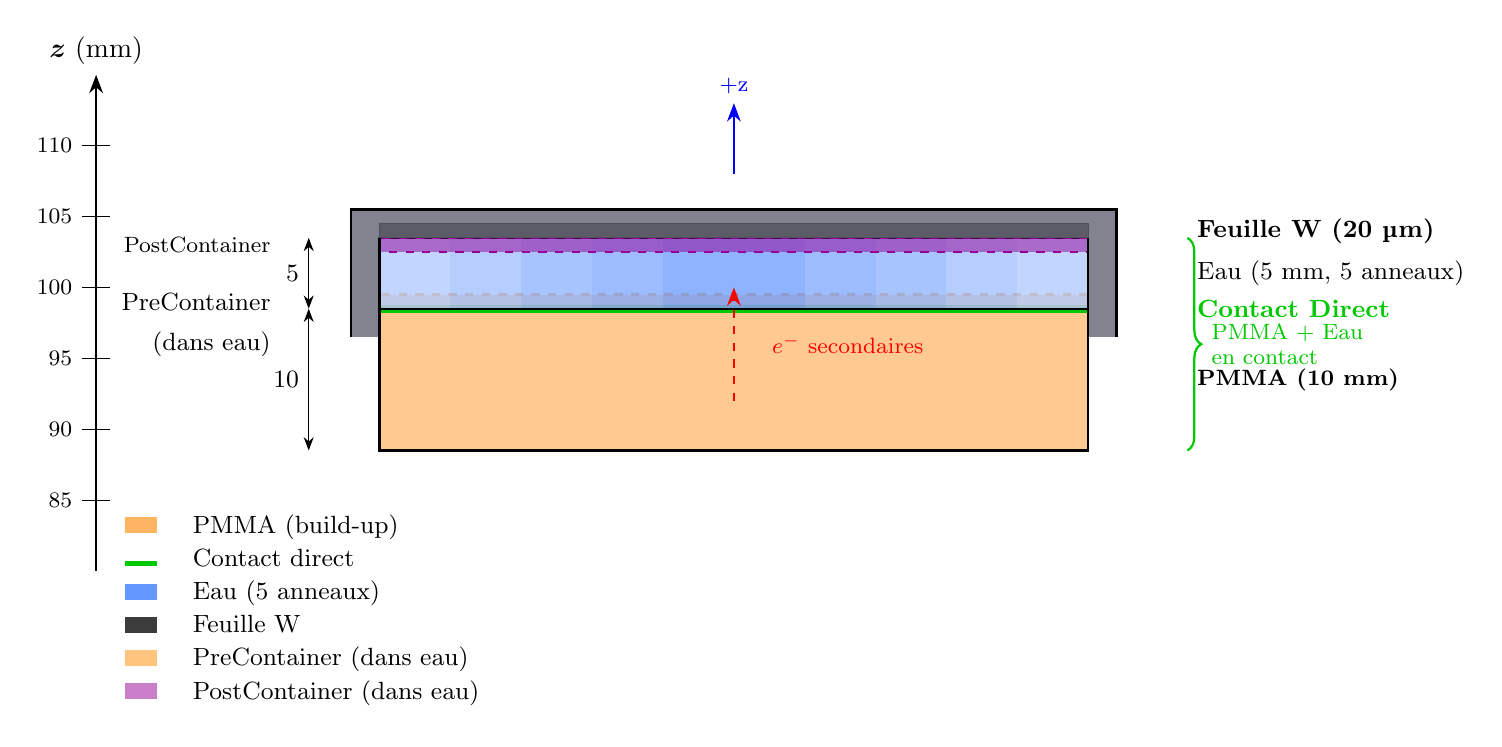
\begin{tikzpicture}[scale=0.18, >=Stealth]

    % ═══════════════════════════════════════════════════════════════════════════
    % DÉFINITION DES COULEURS
    % ═══════════════════════════════════════════════════════════════════════════
    \definecolor{sourcecolor}{RGB}{255, 50, 50}
    \definecolor{filtercolor}{RGB}{120, 120, 140}
    \definecolor{containercolor}{RGB}{100, 100, 115}
    \definecolor{pmmacolor}{RGB}{255, 180, 100}
    \definecolor{watercolor}{RGB}{100, 150, 255}
    \definecolor{tungstencolor}{RGB}{60, 60, 60}
    \definecolor{precontainercolor}{RGB}{255, 140, 0}
    \definecolor{postcontainercolor}{RGB}{150, 0, 150}
    \definecolor{contactcolor}{RGB}{0, 200, 0}

    % ═══════════════════════════════════════════════════════════════════════════
    % AXE Z (vertical)
    % ═══════════════════════════════════════════════════════════════════════════
    \draw[->, thick] (-45, 80) -- (-45, 115) node[above] {$\bm{z}$ (mm)};
    
    % Graduations
    \foreach \z in {85, 90, 95, 100, 105, 110} {
        \draw (-46, \z) -- (-44, \z);
        \node[left] at (-46, \z) {\footnotesize \z};
    }

    % ═══════════════════════════════════════════════════════════════════════════
    % PMMA (z = 88.5 - 98.5 mm) - 10 mm EN CONTACT DIRECT
    % ═══════════════════════════════════════════════════════════════════════════
    \fill[pmmacolor, opacity=0.7] (-25, 88.5) rectangle (25, 98.5);
    \draw[black, thick] (-25, 88.5) rectangle (25, 98.5);
    \node[right] at (32, 93.5) {\footnotesize \textbf{PMMA (10 mm)}};
    
    % Cotation PMMA
    \draw[<->, thin] (-30, 88.5) -- (-30, 98.5);
    \node[left] at (-30, 93.5) {\small 10};

    % ═══════════════════════════════════════════════════════════════════════════
    % ZONE DE CONTACT PMMA-EAU (ligne verte épaisse)
    % ═══════════════════════════════════════════════════════════════════════════
    \draw[contactcolor, line width=3pt] (-25, 98.5) -- (25, 98.5);
    \node[contactcolor, right] at (32, 98.5) {\small \textbf{Contact Direct}};

    % ═══════════════════════════════════════════════════════════════════════════
    % PreContainerPlane (z = 98.5 - 99.5 mm) - DANS L'EAU
    % ═══════════════════════════════════════════════════════════════════════════
    \fill[precontainercolor, opacity=0.5] (-25, 98.5) rectangle (25, 99.5);
    \draw[precontainercolor, thick, dashed] (-25, 98.5) rectangle (25, 99.5);
    \node[left] at (-32, 99) {\small PreContainer};
    \node[left] at (-32, 96) {\small (dans eau)};

    % ═══════════════════════════════════════════════════════════════════════════
    % EAU - 5 anneaux (z = 98.5 - 103.5 mm)
    % ═══════════════════════════════════════════════════════════════════════════
    % Anneau 0 (r = 0-5 mm)
    \fill[watercolor!90, opacity=0.8] (-5, 98.5) rectangle (5, 103.5);
    % Anneau 1 (r = 5-10 mm)
    \fill[watercolor!80, opacity=0.8] (-10, 98.5) rectangle (-5, 103.5);
    \fill[watercolor!80, opacity=0.8] (5, 98.5) rectangle (10, 103.5);
    % Anneau 2 (r = 10-15 mm)
    \fill[watercolor!70, opacity=0.8] (-15, 98.5) rectangle (-10, 103.5);
    \fill[watercolor!70, opacity=0.8] (10, 98.5) rectangle (15, 103.5);
    % Anneau 3 (r = 15-20 mm)
    \fill[watercolor!60, opacity=0.8] (-20, 98.5) rectangle (-15, 103.5);
    \fill[watercolor!60, opacity=0.8] (15, 98.5) rectangle (20, 103.5);
    % Anneau 4 (r = 20-25 mm)
    \fill[watercolor!50, opacity=0.8] (-25, 98.5) rectangle (-20, 103.5);
    \fill[watercolor!50, opacity=0.8] (20, 98.5) rectangle (25, 103.5);
    
    \draw[black, thick] (-25, 98.5) rectangle (25, 103.5);
    \node[right] at (32, 101) {\small Eau (5 mm, 5 anneaux)};
    
    % Cotation eau
    \draw[<->, thin] (-30, 98.5) -- (-30, 103.5);
    \node[left] at (-30, 101) {\small 5};

    % ═══════════════════════════════════════════════════════════════════════════
    % PostContainerPlane (z = 102.5 - 103.5 mm) - DANS L'EAU
    % ═══════════════════════════════════════════════════════════════════════════
    \fill[postcontainercolor, opacity=0.5] (-25, 102.5) rectangle (25, 103.5);
    \draw[postcontainercolor, thick, dashed] (-25, 102.5) rectangle (25, 103.5);
    \node[left] at (-32, 103) {\footnotesize PostContainer};

    % ═══════════════════════════════════════════════════════════════════════════
    % FEUILLE DE TUNGSTÈNE (z = 103.5 - 103.52 mm, 20 µm)
    % ═══════════════════════════════════════════════════════════════════════════
    \fill[tungstencolor] (-25, 103.5) rectangle (25, 104.5);  % Exagéré pour visibilité
    \draw[black] (-25, 103.5) rectangle (25, 104.5);
    \node[right] at (32, 104) {\small \textbf{Feuille W (20 µm)}};

    % ═══════════════════════════════════════════════════════════════════════════
    % CONTAINER W/PETG (parois latérales et couvercle)
    % ═══════════════════════════════════════════════════════════════════════════
    % Paroi gauche
    \fill[containercolor, opacity=0.8] (-27, 96.5) rectangle (-25, 103.5);
    % Paroi droite
    \fill[containercolor, opacity=0.8] (25, 96.5) rectangle (27, 103.5);
    % Couvercle
    \fill[containercolor, opacity=0.8] (-27, 103.5) rectangle (27, 105.5);
    
    \draw[black, thick] (-27, 96.5) -- (-27, 105.5) -- (27, 105.5) -- (27, 96.5);
    \draw[black, thick] (-25, 96.5) -- (-25, 103.5);
    \draw[black, thick] (25, 96.5) -- (25, 103.5);

    % ═══════════════════════════════════════════════════════════════════════════
    % LÉGENDE
    % ═══════════════════════════════════════════════════════════════════════════
    \node[anchor=north west] at (-45, 85) {
        \begin{tabular}{cl}
            \tikz\fill[pmmacolor] (0,0) rectangle (0.4,0.2); &\small PMMA (build-up) \\
            \tikz\draw[contactcolor, line width=2pt] (0,0.1) -- (0.4,0.1); &\small Contact direct \\
            \tikz\fill[watercolor] (0,0) rectangle (0.4,0.2); &\small Eau (5 anneaux) \\
            \tikz\fill[tungstencolor] (0,0) rectangle (0.4,0.2); &\small Feuille W \\
            \tikz\fill[precontainercolor, opacity=0.5] (0,0) rectangle (0.4,0.2); &\small PreContainer (dans eau) \\
            \tikz\fill[postcontainercolor, opacity=0.5] (0,0) rectangle (0.4,0.2); &\small PostContainer (dans eau) \\
        \end{tabular}
    };

    % ═══════════════════════════════════════════════════════════════════════════
    % ANNOTATIONS
    % ═══════════════════════════════════════════════════════════════════════════
    
    % Accolade pour montrer le contact
    \draw[decorate, decoration={brace, amplitude=5pt, mirror}, thick, contactcolor] 
        (32, 88.5) -- (32, 103.5) node[midway, right=5pt, align=left] {\footnotesize PMMA + Eau\\[-1mm]\footnotesize en contact};
    
    % Flèche pour les électrons
    \draw[->, thick, red, dashed] (0, 92) -- (0, 100);
    \node[red, right] at (2, 96) {\footnotesize $e^-$ secondaires};
    
    % Flèche direction +z
    \draw[->, thick, blue] (0, 108) -- (0, 113);
    \node[blue, above] at (0, 113) {\footnotesize +z};

\end{tikzpicture}
\captionsetup{labelformat=empty}
\caption{\footnotesize Coupe schématique du container avec PMMA de 10 mm en contact direct avec l'eau. Les plans de comptage (PreContainer et PostContainer) sont maintenant dans l'eau (chevauchement autorisé). Les électrons secondaires créés dans le PMMA peuvent atteindre directement l'eau.}
\end{figure}

\begin{table}[H]
\centering
\captionsetup{labelformat=empty}
\caption{\footnotesize Positions détaillées des éléments du container}
\begin{tabular}{@{}lccl@{}}
\toprule
\footnotesize \textbf{Élément}&\footnotesize \textbf{$z_{\min}$ (mm)}&\footnotesize \textbf{$z_{\max}$ (mm)}&\footnotesize \textbf{Remarque} \\
\midrule
\multicolumn{4}{c}{\footnotesize \textit{Empilement depuis la source ($+z$)}} \\
\midrule
\footnotesize PMMA&\footnotesize 88.5&\footnotesize 98.5&\footnotesize Face supérieure = bas de l'eau \\
\rowcolor{green!10}
\footnotesize \textbf{Interface PMMA/Eau}&\multicolumn{2}{c}{\footnotesize \textbf{z = 98.5}}&\footnotesize \textbf{Contact direct !} \\
\footnotesize Eau&\footnotesize 98.5&\footnotesize 103.5&\footnotesize 5 anneaux concentriques \\
\footnotesize PreContainerPlane&\footnotesize  98.5&\footnotesize 99.5&\footnotesize \textcolor{orange}{Dans l'eau (chevauche)} \\
\footnotesize PostContainerPlane&\footnotesize  102.5&\footnotesize 103.5&\footnotesize \textcolor{violet}{Dans l'eau (chevauche)} \\
\footnotesize Feuille W&\footnotesize 103.5&\footnotesize  103.52&\footnotesize Sur l'eau \\
\footnotesize Couvercle container&\footnotesize 103.5&\footnotesize 105.5&\footnotesize W/PETG \\
\bottomrule
\end{tabular}
\end{table}


\normalsize
\noindent \color{blue}\textbf{Figure PreContainer (4 panneaux)}\color{black}
\footnotesize
\medskip

\begin{figure}[H]
\centering
\includegraphics[scale=0.35]{Figures/histos_precontainer_Contact.png}
\captionsetup{labelformat=empty}
\caption{\footnotesize \textbf{Photons (panneaux supérieurs)}\newline 
\textbf{Électrons (panneaux inférieurs)}}
\end{figure}

\medskip
\normalsize
\noindent \color{blue}\textbf{Figure Comparaison Pre/Post (photons)}\color{black}
\footnotesize

\medskip
\begin{figure}[H]
\centering
\includegraphics[scale=0.35]{Figures/histos_comparison_photons_Contact.png}
\captionsetup{labelformat=empty}
\caption{\footnotesize Spectres Photon Pre et Post containers}
\end{figure}

\medskip
\normalsize
\noindent \color{blue}\textbf{Figure Photons backscatter}\color{black}
\footnotesize 
\medskip

\begin{figure}[H]
\centering
\includegraphics[scale=0.35]{Figures/histos_postcontainer_photons_backscatter_Contact.png}
\captionsetup{labelformat=empty}
\end{figure}

\medskip
\normalsize
\noindent \color{blue}\textbf{Figure Électrons transmis}\color{black}
\footnotesize
\medskip

\begin{figure}[H]
\centering
\includegraphics[scale=0.4]{Figures/histos_postcontainer_photons_transmis_Contact.png}
\captionsetup{labelformat=empty}
\end{figure}
 
\medskip
\normalsize
\noindent \color{blue}\textbf{Figure Électrons backscatter}\color{black}
\footnotesize
\medskip

\begin{figure}[H]
\centering
\includegraphics[scale=0.38]{Figures/histos_postcontainer_electrons_backscatter_Contact.png}
\captionsetup{labelformat=empty}
\end{figure}

\medskip
\normalsize
\noindent \color{blue}\textbf{Figure Électrons transmis}\color{black}
\footnotesize
\medskip

\begin{figure}[H]
\centering
\includegraphics[scale=0.38]{Figures/histos_postcontainer_electrons_transmis_Contact.png}
\captionsetup{labelformat=empty}
\end{figure}

\clearpage

\medskip
\normalsize
\noindent \color{blue}\textbf{Distribution radiale de la dose}\color{black}
\footnotesize
\medskip

\begin{figure}[H]
\centering
\includegraphics[width=0.5\textwidth]{Figures/dose_vs_rayon_Contact.png}
\captionsetup{labelformat=empty}
\caption{\footnotesize Dose moyenne par désintégration en fonction du rayon. Les points représentent la dose moyenne calculée sur 25 millions d'événements. La dose varie entre \SI{1.28e-6}{nGy} et \SI{1.22e-6}{nGy}, soit une variation relative de seulement 6\%.}
\end{figure}

\medskip
\normalsize
\noindent \color{blue}\textbf{Distributions de dose par événement}\color{black}
\footnotesize
\medskip

\begin{figure}[H]
\centering
\includegraphics[width=1.0\textwidth]{Figures/histos_dose_par_anneau_Contact.png}
\captionsetup{labelformat=empty}
\caption{\footnotesize Distributions de la dose par désintégration pour chaque anneau. L'échelle verticale est logarithmique. Le panneau inférieur droit présente le résumé des doses totales.}
\end{figure}

\medskip
\normalsize
\noindent \color{blue}\textbf{Distributions de dose total}\color{black}
\footnotesize
\medskip

\begin{figure}[H]
\centering
\includegraphics[width=0.45\textwidth]{Figures/histos_dose_totale_Contact.png}
\captionsetup{labelformat=empty}
\caption{\footnotesize Distributions de la dose total par désintégration. L'échelle verticale est logarithmique.}
\end{figure}

\begin{figure}[H]
\centering
\includegraphics[width=0.55\textwidth]{Figures/histos_dose_comparaison_Contact.png}
\captionsetup{labelformat=empty}
\caption{\footnotesize Superposition des distributions de dose pour les 5 anneaux. Les distributions sont similaires en forme mais décalées vers les faibles doses pour les anneaux extérieurs.}
\end{figure}


\begin{tcolorbox}[colback=blue!5,colframe=blue,title=\textbf{Comparaison avec ou sans PMMA}]
\noindent \textbf{-} \; La figure suivante montre la distribution de la dose déposée dans l'anneau centrale \color{blue}\textbf{avec ou sans}\color{black} \; PMMA\par
\noindent \textbf{-} \; L'épaisseur de la plaque de PMMA est de \color{blue}\textbf{10 mm}\color{black}\par
\noindent \textbf{-} \; La plaque de PMMA est au contact de l'eau\par
\noindent \textbf{-} \; Le PreContainer Plane est dans l'eau au contact avec le PMMA
\end{tcolorbox}

\begin{figure}[H]
\centering
\includegraphics[width=0.75\textwidth]{Figures/comparaison_dose_anneau_central_PMMA_10mm_Contact.png}
\captionsetup{labelformat=empty}
\caption{\footnotesize Superposition des distributions de dose l'anneau cental avec ou sans bloc de PMMA de 10 mm au contact}
\end{figure}


\clearpage

%==============================================================================
\normalsize
\noindent \begin{mdframed}[backgroundcolor=orange!20]
\section{\Large \color{blue} \textbf{Changement de position de la source z=20mm à z=60mm}\color{black}}
\end{mdframed}
\footnotesize
%==============================================================================

\begin{tcolorbox}[colback=blue!5,colframe=blue,title=\textbf{Configuration}]
\noindent ${\rm \; \; \; \; \; \; }$ \textbf{-} \; Le \color{blue}\textbf{Filtre est supprimé}\color{black}\par
\noindent ${\rm \; \; \; \; \; \; }$ \textbf{-} \; La source est \color{blue}\textbf{avancée de 40 mm}\color{black}, passant de \color{blue}$\bm{z = 20mm}$\color{black} à \color{blue}$\bm{z = 60mm}$\color{black}\par
\noindent ${\rm \; \; \; \; \; \; }$ \textbf{-} \; L'eau est \color{blue}\textbf{précédée d'une plaque de PMMA de 10 mm d'epaisseur}\color{black}, pour améliorer la conversion des photons incidents et la \color{blue}\textbf{production d'électrons secondaires}\color{black} \; dans l'eau du container. L'objectif de ce plan est d'améliorer le build-up electronique\par
\noindent ${\rm \; \; \; \; \; \; }$ \textbf{-} \; L'eau est au \color{blue}\textbf{contact de la plaque de PMMA}\color{black} \; de 10 mm d'epaisseur,\par
\noindent ${\rm \; \; \; \; \; \; }$ \textbf{-} \; Le fond du container d'eau est tapissé d'une \color{blue}\textbf{feuille de tungstène}\color{black} \; pour améliorer la \color{blue}\textbf{rétrodiffusion des électrons}\color{black} \; produit par les photons incidents dans la feuille de tungsténe. L'objectif de ce plan est d'améliorer le build-up electronique
\end{tcolorbox}


%===============================================================================
\normalsize
\noindent \begin{mdframed}[backgroundcolor=orange!20]
\subsection{\color{blue}\textbf{Nouvelle Géometrie}\color{black}}
\end{mdframed}
\footnotesize
%===============================================================================
\medskip

\begin{figure}[H]
\centering
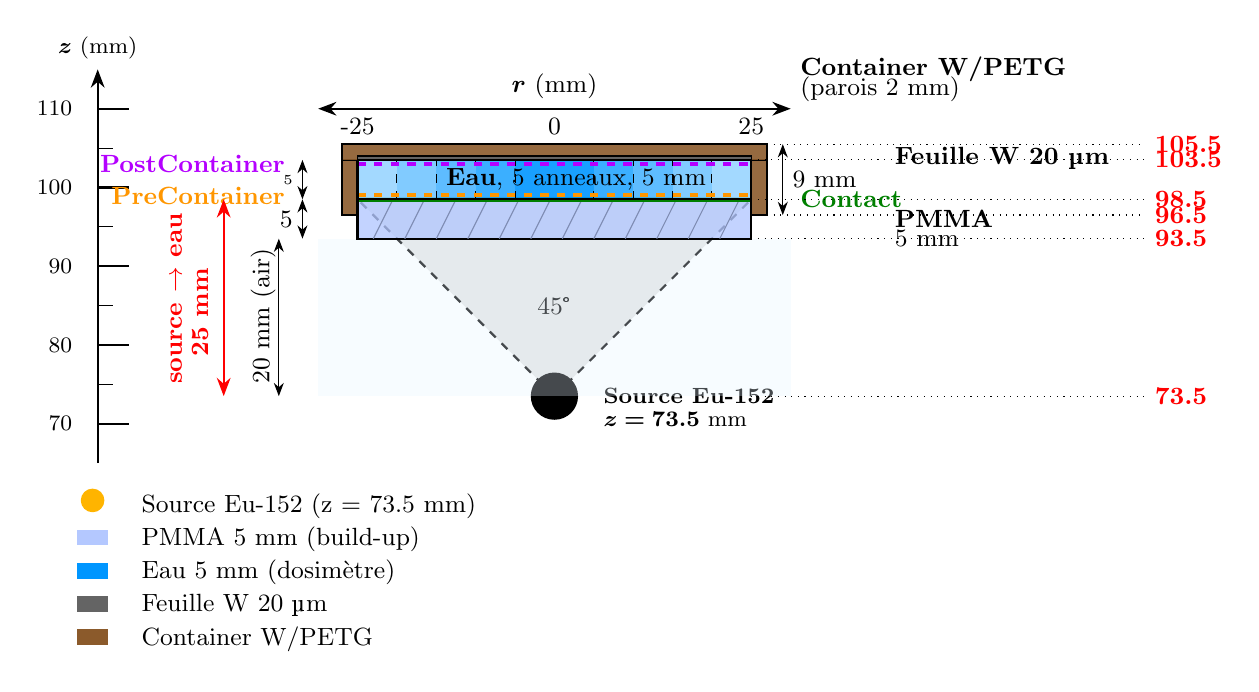
\begin{tikzpicture}[scale=0.1, >=Stealth]

    % ═══════════════════════════════════════════════════════════════════════════
    % DÉFINITION DES COULEURS
    % ═══════════════════════════════════════════════════════════════════════════
    \definecolor{sourcecolor}{RGB}{255, 180, 0}
    \definecolor{aircolor}{RGB}{230, 245, 255}
    \definecolor{pmmacolor}{RGB}{180, 200, 255}
    \definecolor{watercolor}{RGB}{0, 150, 255}
    \definecolor{tungstencolor}{RGB}{100, 100, 100}
    \definecolor{containercolor}{RGB}{139, 90, 43}
    \definecolor{precontainercolor}{RGB}{255, 150, 0}
    \definecolor{postcontainercolor}{RGB}{180, 0, 255}

    % ═══════════════════════════════════════════════════════════════════════════
    % AXE Z (vertical) avec graduations
    % ═══════════════════════════════════════════════════════════════════════════
		
    \draw[->, thick] (-58, 65) -- (-58, 115) node[above] {\footnotesize $\bm{z}$ (mm)};
    
    % Graduations principales
    \foreach \z in {70, 80, 90, 100, 110} {
        \draw[thick] (-58, \z) -- (-54, \z);
        \node[left] at (-60, \z) {\footnotesize \z};
    }
    
    % Graduations secondaires
    \foreach \z in {75, 85, 95, 105} {
        \draw (-58, \z) -- (-56, \z);
    }

    % ═══════════════════════════════════════════════════════════════════════════
    % SOURCE Eu-152 (z = 73.5 mm)
    % ═══════════════════════════════════════════════════════════════════════════
    \fill[black] (0, 73.5) circle (3);
    \node[black, right] at (5, 73.5) {\footnotesize \textbf{Source Eu-152}};
    \node[black, right] at (5, 70.5) {\footnotesize $\bm{z = 73.5}$ mm};
    
    % Cône d'émission (45°)
    % tan(45°) = 1, donc à z=98.5 (d=25), r = 25 mm
    \draw[black, dashed, thick] (0, 73.5) -- (-25, 98.5);
    \draw[black, dashed, thick] (0, 73.5) -- (25, 98.5);
    \fill[black, opacity=0.1] (0, 73.5) -- (-25, 98.5) -- (25, 98.5) -- cycle;
    \node[black] at (0, 85) {\small 45°};

    % ═══════════════════════════════════════════════════════════════════════════
    % AIR entre source et PMMA (z = 73.5 - 93.5 mm)
    % ═══════════════════════════════════════════════════════════════════════════
    \fill[aircolor, opacity=0.3] (-30, 73.5) rectangle (30, 93.5);
    
    % Annotation distance
    \draw[<->, thin, black] (-35, 73.5) -- (-35, 93.5);
    \node[black, left, rotate=90] at (-37, 93.5) {\small 20 mm (air)};

    % ═══════════════════════════════════════════════════════════════════════════
    % PMMA (z = 93.5 - 98.5 mm) - 5 mm
    % ═══════════════════════════════════════════════════════════════════════════
    \fill[pmmacolor, opacity=0.8] (-25, 93.5) rectangle (25, 98.5);
    \draw[black, thick] (-25, 93.5) rectangle (25, 98.5);
    
    % Hachures pour le PMMA
    \foreach \x in {-23,-19,...,23} {
        \draw[pmmacolor!70!black, thin] (\x, 93.5) -- (\x+2.5, 98.5);
    }
    
    \node[right] at (42, 96) {\small \textbf{PMMA}};
    \node[right] at (42, 93.5) {\small 5 mm};
    
    % Cotation PMMA
    \draw[<->, thin] (-32, 93.5) -- (-32, 98.5);
    \node[left] at (-32, 96) {\small 5};

    % ═══════════════════════════════════════════════════════════════════════════
    % INTERFACE PMMA/EAU - Contact direct (z = 98.5 mm)
    % ═══════════════════════════════════════════════════════════════════════════
    \draw[green!50!black, line width=2pt] (-25, 98.5) -- (25, 98.5);
    \node[green!50!black, right] at (30, 98.5) {\small \textbf{Contact}};

    % ═══════════════════════════════════════════════════════════════════════════
    % EAU - 5 anneaux concentriques (z = 98.5 - 103.5 mm)
    % ═══════════════════════════════════════════════════════════════════════════
    
    % Anneau 0 (r = 0-5 mm) - centre
    \fill[watercolor!100, opacity=0.9] (-5, 98.5) rectangle (5, 103.5);
    % Anneau 1 (r = 5-10 mm)
    \fill[watercolor!85, opacity=0.9] (-10, 98.5) rectangle (-5, 103.5);
    \fill[watercolor!85, opacity=0.9] (5, 98.5) rectangle (10, 103.5);
    % Anneau 2 (r = 10-15 mm)
    \fill[watercolor!70, opacity=0.9] (-15, 98.5) rectangle (-10, 103.5);
    \fill[watercolor!70, opacity=0.9] (10, 98.5) rectangle (15, 103.5);
    % Anneau 3 (r = 15-20 mm)
    \fill[watercolor!55, opacity=0.9] (-20, 98.5) rectangle (-15, 103.5);
    \fill[watercolor!55, opacity=0.9] (15, 98.5) rectangle (20, 103.5);
    % Anneau 4 (r = 20-25 mm)
    \fill[watercolor!40, opacity=0.9] (-25, 98.5) rectangle (-20, 103.5);
    \fill[watercolor!40, opacity=0.9] (20, 98.5) rectangle (25, 103.5);
    
    % Contour eau
    \draw[black, thick] (-25, 98.5) rectangle (25, 103.5);
    
    % Séparations des anneaux
    \foreach \r in {-20, -15, -10, -5, 5, 10, 15, 20} {
        \draw[black, thin, dashed] (\r, 98.5) -- (\r, 103.5);
    }
    
    \node[right] at (-15, 101) {\small \textbf{Eau}, 5 anneaux, 5 mm};

    % Cotation eau
    \draw[<->, thin] (-32, 98.5) -- (-32, 103.5);
    \node[left] at (-32, 101) {\tiny 5};

    % ═══════════════════════════════════════════════════════════════════════════
    % PLANS DE COMPTAGE (dans l'eau)
    % ═══════════════════════════════════════════════════════════════════════════
    
    % PreContainerPlane (z = 98.5 - 99.5 mm) - orange
    \draw[precontainercolor, line width=1.5pt, dashed] (-25, 99) -- (25, 99);
    \node[precontainercolor, left] at (-33, 99) {\small \textbf{PreContainer}};
    
    % PostContainerPlane (z = 102.5 - 103.5 mm) - violet
    \draw[postcontainercolor, line width=1.5pt, dashed] (-25, 103) -- (25, 103);
    \node[postcontainercolor, left] at (-33, 103) {\small \textbf{PostContainer}};

    % ═══════════════════════════════════════════════════════════════════════════
    % FEUILLE DE TUNGSTÈNE (z = 103.5 - 103.52 mm, 20 µm)
    % ═══════════════════════════════════════════════════════════════════════════
    \fill[tungstencolor] (-25, 103.5) rectangle (25, 104);  % Exagéré pour visibilité
    \draw[black] (-25, 103.5) rectangle (25, 104);
    \node[right] at (42, 103.75) {\small \textbf{Feuille W 20 µm}};

    % ═══════════════════════════════════════════════════════════════════════════
    % CONTAINER W/PETG (parois et couvercle)
    % Parois: r = 25-27 mm, z = 96.5 - 103.5 mm
    % Couvercle: r = 0-27 mm, z = 103.5 - 105.5 mm
    % ═══════════════════════════════════════════════════════════════════════════
    
    % Paroi gauche (r = 25-27 mm)
    \fill[containercolor, opacity=0.9] (-27, 96.5) rectangle (-25, 103.5);
    \draw[black, thick] (-27, 96.5) rectangle (-25, 103.5);
    
    % Paroi droite
    \fill[containercolor, opacity=0.9] (25, 96.5) rectangle (27, 103.5);
    \draw[black, thick] (25, 96.5) rectangle (27, 103.5);
    
    % Couvercle (z = 103.5 - 105.5 mm)
    \fill[containercolor, opacity=0.9] (-27, 103.5) rectangle (27, 105.5);
    \draw[black, thick] (-27, 103.5) -- (-27, 105.5) -- (27, 105.5) -- (27, 103.5);
    
    % La feuille W est DANS le container, redessinons-la au-dessus
    \fill[tungstencolor] (-25, 103.5) rectangle (25, 104);
    \draw[black, thin] (-25, 103.5) rectangle (25, 104);
    
    \node[right] at (30, 115) {\small \textbf{Container W/PETG}};
    \node[right] at (30, 112.5) {\small (parois 2 mm)};

    % Cotation container
    \draw[<->, thin] (29, 96.5) -- (29, 105.5);
    \node[right] at (29, 101) {\small 9 mm};

    % ═══════════════════════════════════════════════════════════════════════════
    % ANNOTATIONS DES POSITIONS Z
    % ═══════════════════════════════════════════════════════════════════════════
    
    % Lignes de repère à droite
    \draw[black, thin, dotted] (25, 73.5) -- (75, 73.5);
    \node[black, right] at (75, 73.5) {\small \color{red}\textbf{73.5}\color{black}};
    
    \draw[black, thin, dotted] (25, 93.5) -- (75, 93.5);
    \node[black, right] at (75, 93.5) {\small \color{red}\textbf{93.5}\color{black}};
    
    \draw[black, thin, dotted] (27, 96.5) -- (75, 96.5);
    \node[black, right] at (75, 96.5) {\small \color{red}\textbf{96.5}\color{black}};
    
    \draw[black, thin, dotted] (25, 98.5) -- (75, 98.5);
    \node[black, right] at (75, 98.5) {\small \color{red}\textbf{98.5}\color{black}};
    
    \draw[black, thin, dotted] (25, 103.5) -- (75, 103.5);
    \node[black, right] at (75, 103.5) {\small \color{red}\textbf{103.5}\color{black}};
    
    \draw[black, thin, dotted] (27, 105.5) -- (75, 105.5);
    \node[black, right] at (75, 105.5) {\small \color{red}\textbf{105.5}\color{black}};

    % ═══════════════════════════════════════════════════════════════════════════
    % AXE R (horizontal)
    % ═══════════════════════════════════════════════════════════════════════════
    \draw[<->, thick] (-30, 110) -- (30, 110);
    \node[above] at (0, 110) {\small $\bm{r}$ (mm)};
    \node[below] at (-25, 110) {\small -25};
    \node[below] at (0, 110) {\small 0};
    \node[below] at (25, 110) {\small 25};

    % ═══════════════════════════════════════════════════════════════════════════
    % COTATION DISTANCE SOURCE-EAU
    % ═══════════════════════════════════════════════════════════════════════════
    \draw[<->, thick, red] (-42, 73.5) -- (-42, 98.5);  %
    \node[red, left, rotate=90] at (-48, 98) {\small \textbf{source $\rightarrow$ eau}};
		\node[red, left, rotate=90] at (-45, 91) {\small \textbf{25 mm}};

    % ═══════════════════════════════════════════════════════════════════════════
    % LÉGENDE
    % ═══════════════════════════════════════════════════════════════════════════
    \node[anchor=north west] at (-64, 63) {
        \begin{tabular}{cl}
            \tikz\fill[sourcecolor] (0,0) circle (0.15); & \small Source Eu-152 (z = 73.5 mm) \\
            \tikz\fill[pmmacolor] (0,0) rectangle (0.4,0.2); & \small PMMA 5 mm (build-up) \\
            \tikz\fill[watercolor] (0,0) rectangle (0.4,0.2); & \small Eau 5 mm (dosimètre) \\
            \tikz\fill[tungstencolor] (0,0) rectangle (0.4,0.2); & \small Feuille W 20 µm \\
            \tikz\fill[containercolor] (0,0) rectangle (0.4,0.2); & \small Container W/PETG \\
        \end{tabular}
    };
\end{tikzpicture}
\captionsetup{labelformat=empty}
\caption{Coupe longitudinale du dispositif Puits Couronne \textbf{sans filtre}. La source Eu-152 est positionnée à $z = 73.5$ mm avec un cône d'émission de 45° (demi-angle). Le PMMA (5 mm) est en contact direct avec l'eau. Les 5 anneaux d'eau concentriques (nuances de bleu) permettent la mesure de dose radiale.}
\end{figure}

% Définition des couleurs
\definecolor{sourcecolor}{RGB}{255, 220, 150}
\definecolor{aircolor}{RGB}{230, 245, 255}
\definecolor{pmmacolor}{RGB}{200, 215, 255}
\definecolor{watercolor}{RGB}{180, 220, 255}
\definecolor{tungstencolor}{RGB}{200, 200, 200}
\definecolor{containercolor}{RGB}{220, 190, 160}
\definecolor{headercolor}{RGB}{70, 130, 180}



\medskip
\normalsize
\noindent \color{blue}\textbf{Distances caractéristiques}\color{black}
\footnotesize
\medskip

\begin{table}[h!]
\centering
\captionsetup{labelformat=empty}
\caption{\footnotesize Paramètres géométriques de la simulation}
\renewcommand{\arraystretch}{1.4}
\begin{tabular}{>{\columncolor{white}}l c c c c}
\toprule
\rowcolor{headercolor!30}
\footnotesize \textbf{Élément}&\footnotesize \textbf{Position z (mm)}&\footnotesize \textbf{Épaisseur}&\footnotesize \textbf{Rayon (mm)} &\footnotesize \textbf{Matériau} \\
\midrule
\rowcolor{sourcecolor!50}
\footnotesize Source Eu-152&\footnotesize 73.5& ponctuelle &\footnotesize -- &\footnotesize  -- \\
\rowcolor{aircolor!50}
\footnotesize Air&\footnotesize 73.5 $\rightarrow$ 93.5&\footnotesize \SI{20}{mm}&\footnotesize  --&\footnotesize Air \\
\rowcolor{pmmacolor!50}
\footnotesize PMMA (build-up)&\footnotesize  93.5 $\rightarrow$ 98.5 &\footnotesize  \SI{5}{mm} &\footnotesize  25 &\footnotesize  PMMA \\
\rowcolor{watercolor!50}
\footnotesize Eau (dosimètre) &\footnotesize  98.5 $\rightarrow$ 103.5 &\footnotesize  \SI{5}{mm} &\footnotesize  25 &\footnotesize  G4\_WATER \\
\rowcolor{tungstencolor!50}
\footnotesize Feuille W &\footnotesize  103.5 $\rightarrow$ 103.52 &\footnotesize  \SI{20}{\micro m} &\footnotesize  25 &\footnotesize  G4\_W \\
\rowcolor{containercolor!50}
\footnotesize Parois container &\footnotesize  96.5 $\rightarrow$ 103.5 &\footnotesize  \SI{2}{mm} &\footnotesize  25--27 &\footnotesize  W/PETG (75\%/25\%) \\
\rowcolor{containercolor!50}
\footnotesize Couvercle container &\footnotesize  103.5 $\rightarrow$ 105.5 &\footnotesize  \SI{2}{mm} &\footnotesize  0--27 &\footnotesize  W/PETG (75\%/25\%) \\
\bottomrule
\end{tabular}
\end{table}





\clearpage

%===============================================================================
\normalsize
\noindent \begin{mdframed}[backgroundcolor=orange!20]
\subsection{\color{blue}\textbf{Analyse de la génération des événements}\color{black}}
\end{mdframed}
\footnotesize
%===============================================================================
\medskip

\normalsize
\noindent \color{blue}\textbf{Tableau des raies}\color{black}
\footnotesize
\medskip

% Définition des couleurs
\definecolor{headercolor}{RGB}{70, 130, 180}
\definecolor{xraycolor}{RGB}{255, 220, 180}
\definecolor{lowgamma}{RGB}{200, 230, 255}
\definecolor{midgamma}{RGB}{180, 255, 180}
\definecolor{highgamma}{RGB}{255, 200, 200}

\begin{table}[H]
\centering
\captionsetup{labelformat=empty}
\caption{\footnotesize Raies gamma et X de l'Eu-152 simulées (13 raies principales)}
\renewcommand{\arraystretch}{1.3}
\begin{tabular}{c c c c c}
\toprule
\rowcolor{headercolor!30}
\footnotesize \textbf{Index} &\footnotesize  \textbf{Énergie (keV)} &\footnotesize  \textbf{Intensité (\%)} &\footnotesize  \textbf{Type} &\footnotesize  \textbf{Origine} \\
\midrule
\rowcolor{xraycolor}
\footnotesize 0&\footnotesize 39.52&\footnotesize 20.8 &\footnotesize Raie X&\footnotesize  K$\alpha_2$ (Sm) \\
\rowcolor{xraycolor}
\footnotesize 1&\footnotesize 40.12&\footnotesize 37.7&\footnotesize Raie X&\footnotesize K$\alpha_1$ (Sm) \\
\rowcolor{lowgamma}
\footnotesize 2&\footnotesize 121.78&\footnotesize 28.41&\footnotesize$\gamma$&\footnotesize $^{152}$Sm$^*$ \\
\rowcolor{lowgamma}
\footnotesize 3&\footnotesize 244.70&\footnotesize 7.53&\footnotesize $\gamma$&\footnotesize $^{152}$Gd$^*$ \\
\rowcolor{midgamma}
\footnotesize 4&\footnotesize 344.28&\footnotesize 26.59&\footnotesize $\gamma$&\footnotesize $^{152}$Gd$^*$ \\
\rowcolor{midgamma}
\footnotesize 5&\footnotesize 411.12&\footnotesize 2.24&\footnotesize $\gamma$&\footnotesize $^{152}$Sm$^*$ \\
\rowcolor{midgamma}
\footnotesize 6&\footnotesize 443.97&\footnotesize 2.83&\footnotesize $\gamma$&\footnotesize $^{152}$Gd$^*$ \\
\rowcolor{midgamma}
\footnotesize 7&\footnotesize 778.90&\footnotesize 12.97&\footnotesize $\gamma$&\footnotesize $^{152}$Sm$^*$ \\
\rowcolor{midgamma}
\footnotesize 8&\footnotesize 867.38&\footnotesize 4.24&\footnotesize $\gamma$&\footnotesize $^{152}$Gd$^*$ \\
\rowcolor{midgamma}
\footnotesize 9&\footnotesize 964.08&\footnotesize 14.63&\footnotesize $\gamma$&\footnotesize $^{152}$Sm$^*$ \\
\rowcolor{highgamma}
\footnotesize  10&\footnotesize 1085.87&\footnotesize 10.21&\footnotesize $\gamma$&\footnotesize $^{152}$Sm$^*$ \\
\rowcolor{highgamma}
\footnotesize 11 &\footnotesize 1112.07&\footnotesize 13.64&\footnotesize $\gamma$& $^{152}$Sm$^*$ \\
\rowcolor{highgamma}
\footnotesize 12 &\footnotesize 1408.01&\footnotesize 21.01&\footnotesize $\gamma$&\footnotesize $^{152}$Sm$^*$ \\
\midrule
\multicolumn{2}{c}{\footnotesize \textbf{TOTAL}} &\footnotesize  \textbf{202.78} & & \\
\bottomrule
\end{tabular}
\end{table}

\vspace{0.3cm}

\noindent\textbf{Légende des couleurs :}
\begin{itemize}
\item \colorbox{xraycolor}{Raies X} : Fluorescence K du Samarium (E $<$ 50 keV)
\item \colorbox{lowgamma}{$\gamma$ basse énergie} : E $<$ 250 keV
\item \colorbox{midgamma}{$\gamma$ moyenne énergie} : 250 keV $<$ E $<$ 1000 keV
\item \colorbox{highgamma}{$\gamma$ haute énergie} : E $>$ 1000 keV
\end{itemize}

\medskip
\normalsize
\noindent \color{blue}\textbf{Vérification des intensités par raie}\color{black}
\footnotesize
\medskip

\begin{table}[H]
\centering
\captionsetup{labelformat=empty}
\caption{\footnotesize Comparaison des intensités simulées et attendues pour chaque raie Eu-152}
\renewcommand{\arraystretch}{1.2}
\begin{tabular}{c c c c c c}
\toprule
\rowcolor{headercolor!30}
\footnotesize \textbf{Raie (keV)}&\footnotesize \textbf{Émis}&\footnotesize \textbf{I simulée (\%)}&\footnotesize \textbf{I attendue (\%)}&\footnotesize \textbf{Écart}&\footnotesize \textbf{Statut} \\
\midrule
\footnotesize39.52 (X)&\footnotesize 5 199 989&\footnotesize 20.80&\footnotesize 20.8&\footnotesize $<0.01\%$&\footnotesize \cmark \\
\footnotesize40.12 (X)&\footnotesize 9 426 440&\footnotesize 37.71&\footnotesize 37.7&\footnotesize $<0.01\%$&\footnotesize \cmark \\
\footnotesize121.78&\footnotesize 7 099 951&\footnotesize 28.40&\footnotesize 28.41&\footnotesize $<0.01\%$&\footnotesize \cmark \\
\footnotesize244.70&\footnotesize 1 882 297&\footnotesize 7.53&\footnotesize 7.53&\footnotesize $<0.01\%$&\footnotesize \cmark \\
\footnotesize344.28&\footnotesize 6 649 673&\footnotesize 26.60&\footnotesize 26.59&\footnotesize $<0.01\%$&\footnotesize \cmark \\
\footnotesize411.12&\footnotesize 558 246&\footnotesize 2.23&\footnotesize 2.24&\footnotesize $<0.5\%$&\footnotesize \cmark \\
\footnotesize443.97&\footnotesize 706 678&\footnotesize 2.83&\footnotesize 2.83&\footnotesize $<0.01\%$&\footnotesize \cmark \\
\footnotesize778.90&\footnotesize 3 245 196&\footnotesize 12.98&\footnotesize 12.97&\footnotesize $<0.1\%$&\footnotesize \cmark \\
\footnotesize867.38&\footnotesize 1 060 009&\footnotesize 4.24&\footnotesize 4.24&\footnotesize $<0.01\%$&\footnotesize \cmark \\
\footnotesize964.08&\footnotesize 3 658 532&\footnotesize 14.63&\footnotesize 14.63&\footnotesize $<0.01\%$& \cmark \\
\footnotesize1085.87&\footnotesize 2 551 198&\footnotesize 10.20&\footnotesize 10.21&\footnotesize $<0.1\%$&\footnotesize \cmark \\
\footnotesize1112.07&\footnotesize 3 409 096&\footnotesize 13.64&\footnotesize 13.64&\footnotesize $<0.01\%$&\footnotesize \cmark \\
\footnotesize1408.01&\footnotesize 5 251 762&\footnotesize 21.01&\footnotesize 21.01&\footnotesize $<0.01\%$&\footnotesize \cmark \\
\midrule
\footnotesize\textbf{TOTAL} &\footnotesize \textbf{50 699 067} &\footnotesize \textbf{202.80} &\footnotesize \textbf{202.78} &\footnotesize $<0.01\%$ &\footnotesize \cmark \\
\bottomrule
\end{tabular}
\end{table}

\normalsize
\noindent \color{blue}\textbf{Vérification du nombre de gammas par désintégration}\color{black}
\footnotesize
\medskip

\begin{tcolorbox}[colback=blue!5,colframe=blue!50!black]
\begin{center}
\begin{tabular}{rl}
\footnotesize \textbf{Événements simulés :} &\footnotesize25 000 000 \\
\footnotesize \textbf{Primaires générés :} &\footnotesize 50 699 067 \\
\end{tabular}
\end{center}
\end{tcolorbox}

\noindent Le nombre moyen de gammas par désintégration est :

\begin{equation*}
\bm{\bar{n}_\gamma} = \frac{\bm{50\,699\,067}}{\bm{25\,000\,000}} = \bm{2.028}
\end{equation*}

\noindent Cette valeur correspond à la somme des intensités du spectre Eu-152 :

\begin{equation*}
\sum_{\bm{i}} \bm{I_i} = \bm{202.8}\% \implies \bm{\bar{n}_\gamma} = \bm{2.028} \quad \cmark
\end{equation*}

\begin{tcolorbox}[colback=green!10,colframe=successcolor,title=\textbf{Conclusion}]
La génération des raies Eu-152 est \textbf{parfaitement cohérente}. Toutes les intensités sont reproduites avec une précision meilleure que 0.5\%.
\end{tcolorbox}

%===============================================================================
\normalsize
\noindent \begin{mdframed}[backgroundcolor=orange!20]
\subsection{\color{blue}\textbf{Angle Solide}\color{black}}
\end{mdframed}
\footnotesize
%===============================================================================
\medskip

\normalsize
\noindent \color{blue}\textbf{Définition de l'angle solide}\color{black}
\footnotesize
\medskip

\noindent L'angle solide $\bm{\Omega}$ est la mesure bidimensionnelle de la portion de sphère vue  depuis un point. Pour une sphère complète :

\begin{equation*}
\bm{\Omega_{4\pi}} = \bm{4\pi} \text{ sr (stéradians)}
\end{equation*}

\noindent Pour un cône de demi-angle $\bm{\theta_0}$ autour de l'axe $\bm{z}$, l'angle solide est :

\begin{equation*}
\bm{\Omega_{\text{cône}}} = \int_{\bm{0}}^{\bm{2\pi}} \bm{d\phi} \int_0^{\bm{\theta_0}} \sin\bm{\theta} \, \bm{d\theta} = \bm{2\pi} (\bm{1} - \cos\bm{\theta_0})
\end{equation*}

\noindent Avec un demi-angle $\bm{\theta_0} = \bm{45}^{\circ}$ :

\begin{equation*}
\bm{\Omega_{\text{cône}}} = \bm{2\pi} (\bm{1 }- \cos \bm{45}^{\circ}) = \bm{2\pi} (\bm{1} - \bm{0.707}) = \bm{2\pi} \times \bm{0.293} = \bm{1.84} \text{ sr}
\end{equation*}

\noindent La \color{blue}\textbf{fraction d'angle solide}\color{black} couverte par le cône est :

\begin{equation*}
\bm{f_\Omega} = \frac{\bm{\Omega_{\text{cône}}}}{\bm{4\pi}} = \frac{\bm{1} - \cos\bm{\theta_0}}{\bm{2}} = \frac{\bm{1} - \cos \bm{45}^{\circ}}{\bm{2}} = \bm{0.146} = \bm{14.6}\%
\end{equation*}

\medskip
\normalsize
\noindent \color{blue}\textbf{Géométrie des angles solides}\color{black}
\footnotesize
\medskip

\begin{figure}[H]
\centering
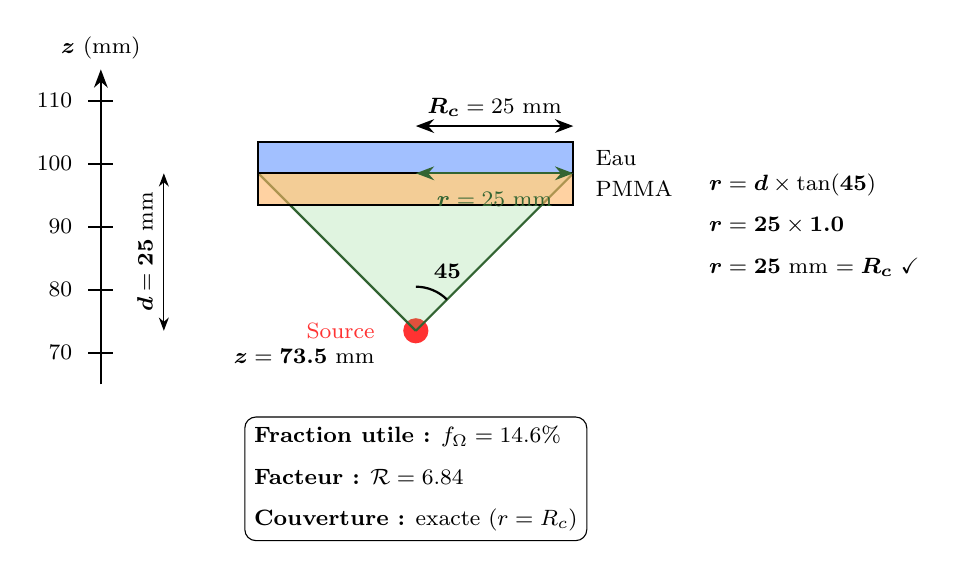
\begin{tikzpicture}[scale=0.08, >=Stealth]

    % ═══════════════════════════════════════════════════════════════════════════
    % AXE Z
    % ═══════════════════════════════════════════════════════════════════════════
    
    \draw[->, thick] (-50, 65) -- (-50, 115) node[above] {\footnotesize $\bm{z}$ (mm)};
    \foreach \z in {70, 80, 90, 100, 110} {
        \draw[thick] (-52, \z) -- (-48, \z);
        \node[left] at (-53, \z) {\footnotesize \z};
    }
    
    % ═══════════════════════════════════════════════════════════════════════════
    % SOURCE
    % ═══════════════════════════════════════════════════════════════════════════
    
    \fill[sourcecolor] (0, 73.5) circle (2);
    \node[sourcecolor, left] at (-5, 73.5) {\footnotesize Source};
    \node[left] at (-5, 69.5) {\footnotesize $\bm{z} = \bm{73.5}$ mm};
    
    % ═══════════════════════════════════════════════════════════════════════════
    % CÔNE D'ÉMISSION
    % ═══════════════════════════════════════════════════════════════════════════
    
    % tan(45°) = 1.0, à d=25mm : r = 25mm
    \fill[usefulcolor, opacity=0.2] (0, 73.5) -- (-25, 98.5) -- (25, 98.5) -- cycle;
    \draw[usefulcolor!50!black, thick] (0, 73.5) -- (-25, 98.5);
    \draw[usefulcolor!50!black, thick] (0, 73.5) -- (25, 98.5);
    
    % Angle
    \draw[thick] (0, 80.5) arc (90:45:7);
    \node at (5, 83) {\footnotesize $\bm{45}°$};
    
    % ═══════════════════════════════════════════════════════════════════════════
    % PMMA
    % ═══════════════════════════════════════════════════════════════════════════
    
    \fill[pmmacolor, opacity=0.6] (-25, 93.5) rectangle (25, 98.5);
    \draw[black, thick] (-25, 93.5) rectangle (25, 98.5);
    \node[right] at (27, 96) {\footnotesize PMMA};
    
    % ═══════════════════════════════════════════════════════════════════════════
    % EAU
    % ═══════════════════════════════════════════════════════════════════════════
    
    \fill[watercolor, opacity=0.6] (-25, 98.5) rectangle (25, 103.5);
    \draw[black, thick] (-25, 98.5) rectangle (25, 103.5);
    \node[right] at (27, 101) {\footnotesize Eau};
    
    % Parois
    \draw[black, thick] (-25, 93.5) -- (-25, 103.5);
    \draw[black, thick] (25, 93.5) -- (25, 103.5);
    
    % ═══════════════════════════════════════════════════════════════════════════
    % RAYONS
    % ═══════════════════════════════════════════════════════════════════════════
    
    % Rayon container
    \draw[<->, thick] (0, 106) -- (25, 106);
    \node[above] at (12.5, 106) {\footnotesize $\bm{R_c} = 25$ mm};
    
    % Rayon cône (= rayon container à z=98.5)
    \draw[<->, usefulcolor!50!black, thick] (0, 98.5) -- (25, 98.5);
    \node[usefulcolor!50!black, below] at (12.5, 97) {\footnotesize $\bm{r} = 25$ mm};
    
    % Distance source -> eau
    \draw[<->, black] (-40, 73.5) -- (-40, 98.5);
    \node[black, rotate=90] at (-43, 86) {\footnotesize $\bm{d} = \bm{25}$ mm};
    
    % ═══════════════════════════════════════════════════════════════════════════
    % FORMULES
    % ═══════════════════════════════════════════════════════════════════════════
    
    \node[anchor=north west, align=left] at (45, 100) {
        \footnotesize $\bm{r} = \bm{d} \times \tan(\bm{45}°)$\\[3pt]
        \footnotesize $\bm{r} = \bm{25} \times \bm{1.0}$\\[3pt]
        \footnotesize $\bm{r} = \bm{25}$ mm $= \bm{R_c}$ \checkmark
    };
    
    % ═══════════════════════════════════════════════════════════════════════════
    % ENCADRÉ
    % ═══════════════════════════════════════════════════════════════════════════
    
    \node[draw, fill=white, rounded corners, align=left] at (0, 50) {
        \footnotesize \textbf{Fraction utile :} $f_\Omega = 14.6\%$\\[3pt]
        \footnotesize \textbf{Facteur :} $\mathcal{R} = 6.84$\\[3pt]
        \footnotesize \textbf{Couverture :} exacte ($r = R_c$)
    };

\end{tikzpicture}
\captionsetup{labelformat=empty}
\caption{\footnotesize Géométrie du cône d'émission. Le cône de 45° couvre exactement le rayon du container (25 mm) au niveau de l'entrée de l'eau. La couverture est optimale.}
\end{figure}

\begin{center}
\fbox{
\parbox{0.85\textwidth}{
\centering
\textbf{\large \color{blue}\textbf{Angle solide et renormalisation}\color{black}}\\[10pt]

\begin{tabular}{rl}
\color{blue}\textbf{Problème :}\color{black} & Une source réelle émet dans toutes les directions ($\bm{4\pi}$)\\[3pt]
& $\Rightarrow$ La plupart des gammas ne touchent pas le détecteur\\[8pt]

\color{blue}\textbf{Solution :}\color{black} & Simuler uniquement un cône dirigé vers le détecteur\\[3pt]
& $\Rightarrow$ Gain de temps de calcul considérable\\[8pt]

\color{blue}\textbf{Fraction utile :}\color{black}& $\bm{f_\Omega} = \dfrac{\bm{1} - \cos(\bm{45}°)}{2} = \bm{14.6}\%$\\[10pt]

\color{blue}\textbf{Équivalence :}\color{black}& 1 evt simulation = 0.146 désintégration réelle\\[3pt]
& 6.84 evt simulation = 1 désintégration réelle\\[8pt]

\color{blue}\textbf{Conversion dose :}\color{black}& $\bm{D_{\text{réelle}}} = \bm{D_{\text{simulation}}} \times 0.146$\\[8pt]

\color{blue}\textbf{Temps irradiation :}\color{black}& $\bm{t} = \dfrac{\bm{N_{\text{evt}}} \times \bm{6.84}}{\bm{A}}$ (avec $\bm{A}$ en Bq)
\end{tabular}
}
}
\end{center}

\medskip
\normalsize
\noindent \color{blue}\textbf{Vérification de la couverture géométrique}\color{black}
\footnotesize
\medskip

\noindent Le rayon couvert par le cône à la distance $\bm{d}$ de la source est :

\begin{equation*}
\bm{r_{\text{cône}}}(\bm{d}) = \bm{d} \times \tan\bm{\theta_0}
\end{equation*}

\begin{table}[H]
\centering
\captionsetup{labelformat=empty}
\caption{\footnotesize Rayon couvert par le cône ($\theta_0 = 45^{\circ}$) à différentes positions}
\begin{tabular}{@{}l c c c c@{}}
\toprule
\footnotesize\textbf{Position}&\footnotesize $z$ \textbf{(mm)}&\footnotesize $d = z - z_s$ \textbf{(mm)}&\footnotesize $r_{\text{cône}}$ \textbf{(mm)}&\footnotesize \textbf{Couverture} \\
\midrule
\footnotesize Bas PMMA&\footnotesize 93.5&\footnotesize 20.0&\footnotesize 20.0&\footnotesize $< R_c$ \\
\rowcolor{watercolor!20}
\footnotesize Bas eau&\footnotesize 98.5&\footnotesize 25.0&\footnotesize \textbf{25.0}&\footnotesize $= R_c$ \\
\footnotesize Centre eau&\footnotesize 101.0&\footnotesize 27.5&\footnotesize 27.5&\footnotesize $> R_c$  \\
\footnotesize Haut eau &\footnotesize 103.5&\footnotesize 30.0&\footnotesize 30.0&\footnotesize $> R_c$  \\
\bottomrule
\end{tabular}
\end{table}

\begin{tcolorbox}[colback=blue!5,colframe=blue,title=\textbf{Conclusion}]
\noindent Le cône de $45^{\circ}$ couvre exactement le container d'eau ($\bm{R_c} = 25$ mm) à l'entrée de l'eau ($z = 98.5$ mm), puis dépasse dans l'épaisseur de l'eau avec une marge croissante jusqu'à $+5$ mm en sortie.
\end{tcolorbox}

%===============================================================================
\normalsize
\noindent \begin{mdframed}[backgroundcolor=orange!20]
\subsection{\color{blue}\textbf{Renormalisation}\color{black}}
\end{mdframed}
\footnotesize
%===============================================================================
\medskip

\noindent Dans une simulation Monte Carlo d'une source isotrope (émission $\bm{4\pi}$), la grande majorité des particules n'atteint jamais le détecteur. Pour optimiser le temps de calcul, on restreint l'émission à un cône dirigé vers la région d'intérêt.\par
\medskip
\noindent Pour que les résultats de la simulation avec cône soient équivalents à une source isotrope réelle, il faut appliquer un \color{blue}\textbf{facteur de renormalisation}.\color{black}\par
\medskip
\noindent Une source d'activité $\bm{A}$ (en Bq) émet $\bm{A}$ désintégrations par seconde dans tout l'espace $\bm{4\pi}$. Le nombre de gammas émis vers l'angle solide $\bm{\Omega}$ est :
\begin{equation*}
\bm{\dot{N}_\gamma}^{\bm{\Omega}} = \bm{A} \times \bm{\bar{n}_\gamma} \times \frac{\bm{\Omega}}{\bm{4\pi}}
\end{equation*}
\noindent où $\bm{\bar{n}_\gamma}$ est le nombre moyen de gammas par désintégration.
\medskip
\noindent Dans la simulation, \textbf{tous} les gammas sont émis dans le cône $\bm{}\Omega_{\text{cône}}$. Un événement de simulation correspond donc à une fraction de désintégration :
\begin{equation*}
\bm{1} \text{ événement simulation} \equiv \bm{f_\Omega} \text{ désintégration réelle}
\end{equation*}
\medskip
\normalsize
\noindent \color{blue}\textbf{Facteur de renormalisation}\color{black}
\footnotesize
\medskip
\noindent Le facteur de renormalisation $\bm{\mathcal{R}}$ permet de convertir les résultats de simulation en équivalent physique :
\begin{equation*}
\bm{\mathcal{R}} = \frac{\bm{1}}{\bm{f_\Omega}} = \frac{\bm{2}}{\bm{1} - \cos\bm{\theta_0}} = \frac{\bm{2}}{\bm{1} - \cos \bm{45}^{\circ}} = \frac{\bm{2}}{\bm{0.293}} = \bm{6.83}
\end{equation*}
\begin{tcolorbox}[colback=blue!5,colframe=blue,title=\textbf{Interprétation}]
\noindent Il faut $\bm{\mathcal{R}} = \bm{6.83}$ événements de simulation pour représenter une désintégration complète $4\pi$
\end{tcolorbox}
\clearpage
\medskip
\normalsize
\noindent \color{blue}\textbf{Application aux doses}\color{black}
\footnotesize
\medskip
\noindent La dose par désintégration réelle est :
\begin{equation*}
\bm{D_{\text{réel}}} = \bm{D_{\text{sim}}} \times \bm{f_\Omega} = \frac{\bm{D_{\text{sim}}}}{\bm{\mathcal{R}}}
\end{equation*}
\medskip
\normalsize
\noindent \color{blue}\textbf{Schéma récapitulatif}\color{black}
\footnotesize
\medskip
\begin{figure}[H]
\centering
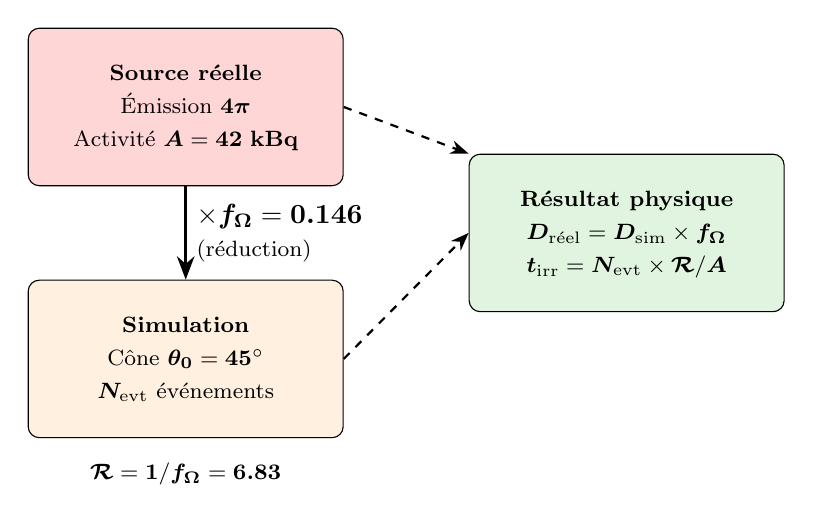
\begin{tikzpicture}[>=Stealth, scale=0.8]
    
    % Boîte source 4\pi
    \node[draw, fill=sourcecolor!20, minimum width=4cm, minimum height=2cm, rounded corners] (source4pi) at (0, 4) {
        \begin{tabular}{c}
            \footnotesize \textbf{Source réelle}\\
            \footnotesize Émission $\bm{4\pi}$\\
            \footnotesize Activité $\bm{A} = \bm{42}$ \textbf{kBq}
        \end{tabular}
    };
    
    % Boîte simulation cône
    \node[draw, fill=conecolor!20, minimum width=4cm, minimum height=2cm, rounded corners] (simcone) at (0, 0) {
        \begin{tabular}{c}
            \footnotesize \textbf{Simulation}\\
            \footnotesize Cône $\bm{\theta_0} = \bm{45}^{\circ}$\\
            \footnotesize $\bm{N_{\text{evt}}}$ \footnotesize événements
        \end{tabular}
    };
    
    % Flèche avec facteur
    \draw[->, very thick] (source4pi) -- (simcone) node[midway, right, align=left] {
        $\times \bm{f_\Omega} = \bm{0.146}$\\
        \footnotesize (réduction)
    };
    
    % Boîte résultat
    \node[draw, fill=solidanglecolor!20, minimum width=4cm, minimum height=2cm, rounded corners] (result) at (7, 2) {
        \begin{tabular}{c}
            \footnotesize \textbf{Résultat physique}\\
            \footnotesize $\bm{D_{\text{réel}}} = \bm{D_{\text{sim}}} \times \bm{f_\Omega}$\\
            \footnotesize $\bm{t_{\text{irr}}} = \bm{N_{\text{evt}}} \times \bm{\mathcal{R}} / \bm{A}$
        \end{tabular}
    };
    
    % Flèches vers résultat
    \draw[->, thick, dashed] (simcone.east) -- (result.west);
    \draw[->, thick, dashed] (source4pi.east) -- (result.north west);
    
    % Annotation
    \node[below] at (0, -1.5) {\footnotesize $\bm{\mathcal{R}} = \bm{1}/\bm{f_\Omega} = \bm{6.83}$};
\end{tikzpicture}
\captionsetup{labelformat=empty}
\caption{\footnotesize Schéma de renormalisation entre simulation (cône) et source réelle ($\bm{4\pi}$).}
\end{figure}

%===============================================================================
% TABLEAU RÉCAPITULATIF DES PARAMÈTRES
%===============================================================================
\medskip
\normalsize
\noindent \color{blue}\textbf{Paramètres de la configuration actuelle}\color{black}
\footnotesize
\medskip

\begin{table}[H]
\centering
\begin{tabular}{|l|c|c|}
\hline
\textbf{Paramètre} & \textbf{Symbole} & \textbf{Valeur} \\
\hline
Activité source (4$\pi$) & $A$ & 42 kBq \\
Demi-angle du cône & $\theta_0$ & 45° \\
Fraction d'angle solide & $f_\Omega = \frac{1-\cos\theta_0}{2}$ & 0.146 (14.6\%) \\
Facteur de renormalisation & $\mathcal{R} = 1/f_\Omega$ & 6.83 \\
Activité effective (dans le cône) & $A_{\text{eff}} = A \times f_\Omega$ & 6.13 kBq \\
\hline
\end{tabular}
\caption{\footnotesize Paramètres de renormalisation pour la simulation.}
\end{table}

%===============================================================================
% APPLICATION NUMÉRIQUE
%===============================================================================
\medskip
\normalsize
\noindent \color{blue}\textbf{Application numérique}\color{black}
\footnotesize
\medskip

\noindent Pour $N_{\text{evt}} = 25 \times 10^6$ événements simulés :
\begin{itemize}
    \item Nombre de désintégrations 4$\pi$ représentées : $N_{\text{désint}} = N_{\text{evt}} \times \mathcal{R} = 25 \times 10^6 \times 6.83 = 171 \times 10^6$
    \item Temps d'irradiation simulé : $t_{\text{irr}} = \frac{N_{\text{désint}}}{A} = \frac{171 \times 10^6}{42 \times 10^3} = 4071$ s $\approx$ \textbf{68 min}
\end{itemize}

\medskip
\noindent Le débit de dose est calculé par :
\begin{equation*}
\dot{D} = D_{\text{sim}} \times A_{\text{eff}} = \frac{D_{\text{sim}}}{N_{\text{evt}}} \times A \times f_\Omega
\end{equation*}






















\medskip
\normalsize
\noindent \color{blue}\textbf{Problème de l'efficacité de simulation}\color{black}
\footnotesize
\medskip

\noindent Dans une simulation Monte Carlo d'une source isotrope (émission $\bm{4\pi}$), la grande majorité des particules n'atteint jamais le détecteur. Pour optimiser le temps de calcul, on restreint l'émission à un cône dirigé vers la région d'intérêt.\par
\medskip
\noindent Pour que les résultats de la simulation avec cône soient équivalents à une source isotrope réelle, il faut appliquer un \color{blue}\textbf{facteur de renormalisation}.\color{black}\par
\medskip
\noindent Une source d'activité $\bm{A}$ (en Bq) émet $\bm{A}$ désintégrations par seconde dans tout l'espace $\bm{4\pi}$. Le nombre de gammas émis vers l'angle solide $\bm{\Omega}$ est :

\begin{equation*}
\bm{\dot{N}_\gamma}^{\bm{\Omega}} = \bm{A} \times \bm{\bar{n}_\gamma} \times \frac{\bm{\Omega}}{\bm{4\pi}}
\end{equation*}

\noindent où $\bm{\bar{n}_\gamma}$ est le nombre moyen de gammas par désintégration.
\medskip
\noindent Dans la simulation, \textbf{tous} les gammas sont émis dans le cône $\bm{}\Omega_{\text{cône}}$. Un événement de simulation correspond donc à une fraction de désintégration :

\begin{equation*}
\bm{1} \text{ événement simulation} \equiv \bm{f_\Omega} \text{ désintégration réelle}
\end{equation*}

\medskip
\normalsize
\noindent \color{blue}\textbf{Facteur de renormalisation}\color{black}
\footnotesize
\medskip

\noindent Le facteur de renormalisation $\bm{\mathcal{R}}$ permet de convertir les résultats de simulation en équivalent physique :

\begin{equation*}
\bm{\mathcal{R}} = \frac{\bm{1}}{\bm{f_\Omega}} = \frac{\bm{2}}{\bm{1} - \cos\bm{\theta_0}} = \frac{\bm{2}}{\bm{1} - \cos \bm{40}^{\circ}} = \frac{\bm{2}}{\bm{0.234}} = \bm{8.55}
\end{equation*}

\begin{tcolorbox}[colback=blue!5,colframe=blue,title=\textbf{Interprétation}]
\noindent Il faut $\bm{\mathcal{R}} = \bm{8.55}$ événements de simulation pour représenter une désintégration complète $4\pi$
\end{tcolorbox}

\clearpage


%===============================================================================
\normalsize
\noindent \begin{mdframed}[backgroundcolor=orange!20]
\subsection{\color{blue}\textbf{Relations activité--temps d'irradiation}\color{black}}
\end{mdframed}
\footnotesize
%===============================================================================












\medskip
\normalsize
\noindent \color{blue}\textbf{Définitions}\color{black}
\footnotesize
\medskip

\begin{itemize}
    \item \color{blue}\textbf{Activité}\color{black} \; $\bm{A}$ : nombre de désintégrations par seconde (Bq)
    \item \color{blue}\textbf{Activité dans le cône}\color{black} \; $\bm{A_{\text{cône}}}$ : désintégrations par seconde contribuant au cône
    \item \color{blue}\textbf{Temps d'irradiation}\color{black} \; $\bm{t_{\text{irr}}}$ : durée nécessaire pour accumuler $\bm{N}$ désintégrations
\end{itemize}

\medskip
\normalsize
\noindent \color{blue}\textbf{Calcul du temps d'irradiation}\color{black}
\footnotesize
\medskip

\noindent \color{red}\textbf{Méthode 1 : À partir des événements simulés}\color{black}\par
\medskip
\noindent Un événement de simulation représente l'émission de gammas dans le cône $\bm{\Omega_{\text{cone}}}$. Pour une source isotrope, cela correspond à une fraction $\bm{f_\Omega}$ de désintégration.\par
\medskip

\noindent Le nombre de désintégrations réelles équivalentes à $\bm{N_{\text{evt}}}$ événements simulés est :

\begin{equation*}
\bm{N_{\text{désint}}} = \frac{\bm{N_{\text{evt}}}}{\bm{f_\Omega}} = \bm{N_{\text{evt}}} \times \bm{\mathcal{R}}
\end{equation*}

\noindent Le temps d'irradiation correspondant est :

\begin{equation*}
\bm{t_{\text{irr}}} = \frac{\bm{N_{\text{désint}}}}{\bm{A}} = \frac{\bm{N_{\text{evt}}} \times \bm{\mathcal{R}}}{\bm{A}} = \frac{\bm{N_{\text{evt}}}}{\bm{A} \times \bm{f_\Omega}}
\end{equation*}

\noindent \color{red}\textbf{Méthode 2 : À partir de l'activité dans le cône}\color{black}\par
\medskip
\noindent  L'activité effective dans le cône est :

\begin{equation*}
\bm{A_{\text{cône}}} = \bm{A} \times \bm{f_\Omega}
\end{equation*}

\noindent Le nombre moyen de gammas émis dans le cône par seconde est :

\begin{equation*}
\bm{\dot{N}_\gamma^{\text{cône}}} = \bm{A_{\text{cône}}} \times \bm{\bar{n}_\gamma} = \bm{A} \times \bm{f_\Omega} \times \bm{\bar{n}_\gamma}
\end{equation*}

\noindent Le temps pour générer $\bm{N_\gamma}$ gammas (= $\bm{N_{\text{primaires}}}$ dans la simulation) est :

\begin{equation*}
\bm{t_{\text{irr}}} = \frac{\bm{N_\gamma}}{\bm{\dot{N}_\gamma^{\text{cône}}}} = \frac{\bm{N_{\text{primaires}}}}{\bm{A} \times \bm{f_\Omega} \times \bm{\bar{n}_\gamma}}
\end{equation*}

\medskip
\normalsize
\noindent \color{blue}\textbf{Application numérique}\color{black}\par
\footnotesize
\medskip

\noindent \color{red}\textbf{Paramètres}\color{black}\par
\medskip

\begin{table}[H]
\centering
\captionsetup{labelformat=empty}
\caption{\footnotesize Paramètres pour le calcul du temps d'irradiation}
\begin{tabular}{@{}l c l@{}}
\toprule
\footnotesize \textbf{Paramètre}&\footnotesize \textbf{Valeur}&\footnotesize \textbf{Source} \\
\midrule
\footnotesize Activité source $\bm{A}$&\footnotesize $4.2 \times 10^4$ Bq&\footnotesize Source Eu-152 \\
&\footnotesize  = 42 kBq& \\
\footnotesize Fraction angle solide $\bm{f_\Omega}$&\footnotesize 0.146&\footnotesize $\bm{\theta_0} = \bm{45}^{\circ}$ \\
\footnotesize Facteur de renormalisation $\bm{\mathcal{R}}$&\footnotesize 6.83&\footnotesize $\bm{1}/\bm{f_\Omega}$ \\
\footnotesize Gammas/désintégration $\bm{\bar{n}_\gamma}$&\footnotesize 2.03&\footnotesize Spectre Eu-152 (13 raies) \\
\footnotesize Événements simulés $\bm{N_{\text{evt}}}$&\footnotesize $25 \times 10^6$&\footnotesize Simulation \\
\footnotesize Primaires générés $\bm{N_{\text{primaires}}}$&\footnotesize $50.7 \times 10^6$&\footnotesize  Simulation \\
\bottomrule
\end{tabular}
\end{table}

\noindent \color{red}\textbf{Calcul par la méthode 1 (événements)}\color{black}
\medskip

\begin{align*}
\bm{N_{\text{désint}}} &= \bm{N_{\text{evt}}} \times \bm{\mathcal{R}} = \bm{25} \times \bm{10^6} \times \bm{6.83} = \bm{170.7} \times \bm{10^6} \text{ désintégrations}\\[10pt]
\bm{t_{\text{irr}}} &= \frac{\bm{N_{\text{désint}}}}{\bm{A}} = \frac{\bm{170.7} \times \bm{10^6}}{\bm{4.2} \times \bm{10^4}} = \bm{4065} \text{ s} = \boxed{\bm{67.7} \text{ min} \approx \bm{1.1} \text{ h}}
\end{align*}

\noindent \color{red}\textbf{Calcul par la méthode 2 (primaires)}\color{black}
\medskip

\begin{align*}
\bm{A_{\text{cône}}} &= \bm{A} \times \bm{f_\Omega} = \bm{4.2} \times \bm{10^4} \times \bm{0.146} = \bm{6.15} \times \bm{10^3} \text{ Bq} = \bm{6.15} \text{ kBq}\\[10pt]
\bm{\dot{N}_\gamma^{\text{cône}}} &= \bm{A_{\text{cône}}} \times \bm{\bar{n}_\gamma} = \bm{6.15} \times \bm{10^3} \times \bm{2.03} = \bm{12.5} \times \bm{10^3} \text{ gammas/s}\\[10pt]
\bm{t_{\text{irr}}} &= \frac{\bm{N_{\text{primaires}}}}{\bm{\dot{N}_\gamma^{\text{cône}}}} = \frac{\bm{50.7} \times \bm{10^6}}{\bm{12.5} \times \bm{10^3}} = \bm{4061} \text{ s} = \boxed{\bm{67.7} \text{ min} \approx \bm{1.1} \text{ h}}
\end{align*}

\begin{tcolorbox}[colback=blue!5,colframe=blue,title=\textbf{Vérification}]
\noindent Les deux méthodes donnent le même résultat : $\bm{t_{\text{irr}} \approx 68}$ \textbf{min} $\approx$ \textbf{1.1 h}
\end{tcolorbox}

\medskip
\normalsize
\noindent \color{blue}\textbf{Tableau récapitulatif des temps d'irradiation}\color{black}
\footnotesize
\medskip

\begin{table}[H]
\centering
\captionsetup{labelformat=empty}
\caption{\footnotesize Temps d'irradiation pour différentes activités de source}
\begin{tabular}{@{}c c c c@{}}
\toprule
\footnotesize \textbf{Activité}&\footnotesize \textbf{Activité}&\footnotesize $t_{\text{irr}}$ \textbf{(25M evt)}&\footnotesize  \textbf{Débit dose (ann. 0)} \\
\footnotesize \textbf{}&\footnotesize  \textbf{}&\footnotesize &\footnotesize \textbf{(µGy/h)} \\
\midrule
\footnotesize 10 kBq&\footnotesize 0.01 MBq&\footnotesize 4.7 h&\footnotesize 1.5 \\
\rowcolor{yellow!20}
\footnotesize \textbf{42 kBq}&\footnotesize \textbf{0.042 MBq}&\footnotesize \textbf{68 min}&\footnotesize \textbf{6.4} \\
\footnotesize 100 kBq&\footnotesize 0.1 MBq&\footnotesize 28.5 min&\footnotesize 15.2 \\
\footnotesize 1 MBq&\footnotesize 1 MBq&\footnotesize 2.8 min&\footnotesize 152 \\
\footnotesize 37 MBq&\footnotesize 37 MBq&\footnotesize 4.6 s&\footnotesize 5 615 \\
\bottomrule
\end{tabular}
\end{table}

\medskip
\normalsize
\noindent \color{blue}\textbf{Formule générale du débit de dose}\color{black}
\footnotesize
\medskip

\noindent Le débit de dose (en µGy/h) est :

\begin{equation*}
\bm{\dot{D}} = \frac{\bm{D_{\text{sim}}}}{\bm{N_{\text{evt}}}} \times \bm{A} \times \bm{f_\Omega} \times \bm{3.6}
\end{equation*}

\noindent où le facteur 3.6 convertit nGy/s en µGy/h (×3600 s/h ÷1000 nGy/µGy).

\medskip
\noindent Application numérique (anneau central, A = 42 kBq) :

\begin{equation*}
\bm{\dot{D}} = \frac{\bm{7196} \text{ nGy}}{\bm{25} \times \bm{10^6}} \times \bm{4.2} \times \bm{10^4} \text{ Bq} \times \bm{0.146} \times \bm{3.6} = \boxed{\bm{6.4} \text{ µGy/h}}
\end{equation*}

\medskip
\normalsize
\noindent \color{blue}\textbf{Temps pour atteindre une dose cible}\color{black}
\footnotesize
\medskip

\noindent Pour atteindre une dose $\bm{D_{\text{cible}}}$ dans l'anneau central :

\begin{equation*}
\bm{t_{\text{cible}}} = \frac{\bm{D_{\text{cible}}}}{\bm{\dot{D}}}
\end{equation*}

\begin{table}[H]
\centering
\captionsetup{labelformat=empty}
\caption{\footnotesize Temps pour atteindre différentes doses (anneau central, A = 42 kBq)}
\begin{tabular}{@{}c c c@{}}
\toprule
\footnotesize \textbf{Dose cible}&\footnotesize \textbf{Temps (heures)}&\footnotesize \textbf{Temps} \\
\midrule
\footnotesize 10 cGy (100 mGy)&\footnotesize 15 625 h&\footnotesize 1.8 ans \\
\rowcolor{yellow!20}
\footnotesize \textbf{20 cGy (200 mGy)}&\footnotesize \textbf{31 250 h}&\footnotesize \textbf{3.6 ans} \\
\footnotesize 50 cGy (500 mGy)&\footnotesize 78 125 h&\footnotesize 8.9 ans \\
\bottomrule
\end{tabular}
\end{table}

\begin{tcolorbox}[colback=red!5,colframe=red,title=\textbf{Conclusion}]
\noindent Avec une source de \textbf{42 kBq}, il faut environ \textbf{3.6 ans} pour atteindre une dose de \textbf{20 cGy} dans l'anneau central.
\end{tcolorbox}












\begin{comment}










% ═══════════════════════════════════════════════════════════════════════════════
\section{Résumé et conclusions}
% ═══════════════════════════════════════════════════════════════════════════════

\subsection{Paramètres clés de la simulation}

\begin{table}[H]
\centering
\caption{Résumé des paramètres de renormalisation}
\begin{tabular}{@{}l c@{}}
\toprule
\textbf{Paramètre} & \textbf{Valeur} \\
\midrule
Demi-angle du cône $\theta_0$ & 40^{\circ} \\
Angle solide du cône $\Omega_{\text{cône}}$ & 1.47 sr \\
Fraction d'angle solide $f_\Omega$ & 11.7\% \\
Facteur de renormalisation $\mathcal{R}$ & 8.55 \\
\midrule
Événements simulés & $25 \times 10^6$ \\
Désintégrations équivalentes & $2.14 \times 10^8$ \\
Temps d'irradiation (1 mCi) & 5.78 s \\
\midrule
Dose totale simulée & 17 390 nGy \\
Dose par désintégration réelle & $8.14 \times 10^{-5}$ nGy \\
Débit de dose (1 mCi) & $\sim 352$ nGy/s \\
\bottomrule
\end{tabular}
\end{table}

\subsection{Formules de conversion}

\begin{center}
\fbox{
\parbox{0.9\textwidth}{
\textbf{Formules essentielles}
\begin{align}
\text{Fraction angle solide :} \quad & f_\Omega = \frac{1 - \cos\theta_0}{2} \\[5pt]
\text{Facteur renormalisation :} \quad & \mathcal{R} = \frac{1}{f_\Omega} = \frac{2}{1 - \cos\theta_0} \\[5pt]
\text{Temps d'irradiation :} \quad & t_{\text{irr}} = \frac{N_{\text{evt}} \times \mathcal{R}}{A} \\[5pt]
\text{Dose réelle :} \quad & D_{\text{réel}} = D_{\text{sim}} \times f_\Omega \\[5pt]
\text{Débit de dose :} \quad & \dot{D} = \frac{D_{\text{sim}} \times A}{N_{\text{evt}} \times \mathcal{R}}
\end{align}
}
}
\end{center}

\subsection{Validation}

\begin{itemize}
    \item[\checkmark] Nombre de gammas par événement : 1.443 (conforme au spectre Eu-152)
    \item[\checkmark] Fraction entrant dans l'eau : 65.7\% (cohérent avec la géométrie)
    \item[\checkmark] Distribution radiale de dose : décroissance physiquement cohérente
    \item[\checkmark] Scaling statistique : $\times 100$ vérifié entre 250k et 25M événements
    \item[\checkmark] Deux méthodes de calcul du temps d'irradiation convergent
\end{itemize}


\end{comment}


\end{document}
